\documentclass[defaultstyle,10pt,master,Helvetica]{thesis}
% Helvetica is a similar font to Arial, with small differences.

%--------------------------------------------------------------
%debug features - some may not be included in the final document
%obter informacao de debug acerca de parêntesis mal fechados
\tracinggroups=1
%\usepackage{showframe}    %show page dimensions, to visually confirm page layout
%\usepackage{showlabels}     %show labels in the printed pdf, for easy finding.
\usepackage{todo} %keep track of things to do in the document
%\usepackage[hide]{todo} %Use this option to remove all todos from the document
%http://tex.stackexchange.com/questions/55618/visual-debugging-of-lengths-in-paragraphs-and-environments
%\usepackage{layouts}  - it is producing a compilation warning
%\usepackage{lua-visual-debug} only compatible with LuaTex
%--------------------------------------------------------------


%% Packages
\typeout{}
\typeout{--------------------------------------------------------------}
\typeout{ +---+ Thesis Template                            }
\typeout{ +---+      Version 2.0, August 2011                         }
\typeout{ +---+  for Instituto Superior Tecnico (IST),                 }
\typeout{ +---+  Universidade Tecnica de Lisboa                         }
\typeout{ * Using Thesis Style form Pedro Tomas                                }
\typeout{ * Created to write Dissertations                             }
\typeout{ * Conforms with IST Master Degree format and with most important packages setup        }
\typeout{ * Should conform with IST PhD Degree format (not verified)   }
\typeout{                                                              }
\typeout{ AUTHOR: Miguel Amador and Joao Marques                                          }
\typeout{ MODIFIED BY: Goncalo Andre                                   }
\typeout{                                                              }
\typeout{ Important: Use all files in the archive, since this is based in all them. Modify dummy files at wish.                                        }
\typeout{--------------------------------------------------------------}
\typeout{}

% Defines an additional alphabet... not required in most cases
% ------------------------------------------------------------
% \DeclareMathAlphabet{\mathpzc}{OT1}{pzc}{m}{it}

% PACKAGE babel:
% ---------------
% The 'babel' package may correct some hyphenisation issues of latex. 
% However in most situations it is not required.
\usepackage[portuguese]{babel}
%\usepackage[fixlanguage]{babelbib} - this does not support ieee bibtex style

% PACKAGE fontenc:
% -----------------
% chooses T1-fonts and allows correct automatic hyphenation.
% from: http://tex.stackexchange.com/questions/664/why-should-i-use-usepackaget1fontenc/677#677
% If you don't use \usepackage[T1]{fontenc},
%   -Words containing accented characters cannot be automatically hyphenated,
%   -You cannot properly copy-and-paste such words from the output (DVI/PS/PDF)
%   -Characters like the pipe sign, less than and greater sign give unexpected results in text.
\usepackage[T1]{fontenc}
% http://tex.stackexchange.com/questions/44694/fontenc-vs-inputenc
% allows the user to input accented characters directly form the keyboard
\usepackage[latin1]{inputenc}
\usepackage{lmodern}

%package verbatim - needed for comment environment
\usepackage{verbatim}

% Package ulem (underlining for emphasis).
% the ulem package provides various types of underlining that can
% stretch between words and be broken across lines.
\usepackage{ulem} % Allows the use of other text emphatizer commands
\normalem % () defines \emph{} back to italic, instead of underline (reverts change from ulem package). 
\raggedbottom %declaration makes all pages the height of the text on that page. No extra vertical space is added. The \flushbottom declaration makes all text pages the same height, adding extra vertical space when necessary to fill out the page.

% PACKAGE date time:
% -----------------
% Lets you alter the format of the date that \today returns.
\usepackage{datetime}
\newdateformat{todaythesis}{%
\monthname[\THEMONTH]  \THEYEAR}

% PACKAGE latexsym:
% -----------------
% Defines additional latex symbols. May be required for thesis with many math symbols.
\usepackage{latexsym}

% PACKAGE amsmath, amsthm, amssymb, amsfonts:
% -------------------------------------------
% This package is typically required. Among many other things it adds the possibility
% to put symbols in bold by using \boldsymbol (not \mathbf); defines additional 
% fonts and symbols; adds the \eqref command for citing equations. I prefer the style
% "(x.xx)" for referering to an equation than to use "equation x.xx".
\usepackage{mathtools}
%\usepackage{amsmath, amsthm, amssymb, amsfonts, amsbsy}
\usepackage{amsthm, amssymb, amsfonts, amsbsy}
%used for the \vrectangleblack in serial terminal examples
\usepackage{stix}

%needed for tikz
\usepackage{standalone} %needed because of floating tickz pictures
\usepackage[usenames,dvipsnames]{xcolor}

% PACKAGE multirow, colortbl, longtable:
% ---------------------------------------
% These packages are most usefull for advanced tables. The first allows to join rows 
% throuhg the command \multirow which works similarly with the command \multicolumn
% The second package allows to color the table (both foreground and background)% The fourth package is only required when tables extend beyond the length of one page;
% The fourth package is only required when tables extend beyond the length of one page;
% with compatibilities with the tabular environment. The third allows the definitions of landscape pages, allowing the use of a different orientation for wider graphics or tables. See package documentation to see the implementation.
\usepackage{multirow}
\usepackage{colortbl}
\usepackage{pdflscape}
%\usepackage{xtab}
\usepackage{longtable}
%\usepackage{afterpage} %needed to avoid longtable page breaks
\usepackage{tabulary}
\usepackage{threeparttable}
%\usepackage{tablefootnote}

% PACKAGE graphics, epsfig, subfigure, caption:
% ---------------------------------------------
% Packages for figures... well you will certainly need these packages, with the exception
% of the 'caption' package. This only allows to define extra caption options.
% Notice that subfigure allows to place figures within figures with its own caption. It
% should be avoided to create an eps file with subfigures. That will mean that you won't be 
% able to reference those subfigures. Instead create an EPS file (the only graphics format supported
% by latex) for each of the subfigures and then use the command \subfigure (see below).
\usepackage{adjustbox}
\usepackage{graphics}
\usepackage{graphicx}
\usepackage{epsfig}
%\usepackage[hang,small,bf]{subfigure} - obsolete package, replace by subcaption
%\usepackage[footnotesize,bf,center]{caption}
\usepackage{dcolumn}
\usepackage{bm}
\usepackage{booktabs}
\usepackage{rotating}
\usepackage{multirow}

\usepackage[font=small,labelfont=bf,textfont=normalfont,justification=centering]{caption}
\usepackage[font=small,labelfont=bf,textfont=normalfont]{subcaption}
%http://tex.stackexchange.com/questions/91566/syntax-similar-to-centering-for-right-and-left/91580#91580?newreg=ab93b1a4f79a4315b773d13d37d37678
%easilly define horizontal orientation of images.
%\usepackage[export]{adjustbox} %causing conflicts - had to find a way around

%include pdf pages in document
\usepackage{pdfpages}

% Improves the interface for defining floating objects such as figures and tables
\usepackage{float}

% PACKAGE listings
% ------------------------------
% This package is used to list source code
\usepackage{listings}

%this package is used for quotations
\usepackage{dirtytalk}

% PACKAGE algorithmic, algorithm
% ------------------------------
% These packages are required if you need to describe an algorithm.
% \usepackage{algorithmic}
% \usepackage[chapter]{algorithm}

% PACKAGE natbib/cite
% -------------------
% The two packages are not compatible, and you should use one of the two. Notice however that the
% IEEE BiBTeX stylesheet is imcompatible with the natbib package. If using the IEEE format, use the 
% cite package instead
\usepackage[square,numbers,sort&compress]{natbib}
%\usepackage{cite}

% PACKAGE acronyum
% -----------------
% This package is most useful for acronyms. The package guarantees that all acronyms definitions are 
% given at the first usage. IMPORTANT: do not use acronyms in titles/captions; otherwise the definition 
% will appear on the table of contents.
\usepackage[printonlyused]{acronym}
\usepackage[titletoc,title,header]{appendix} %modify the titles of appendixes
\usepackage{etoc}       %http://tex.stackexchange.com/questions/228729/how-to-hide-chapter-numbering-in-table-of-contents
%Set page numbering by chapter. The noauto option tells the package not to set pagenumbers: this has to be done by the user
\usepackage[noauto]{chappg}

% PACKAGE extra_functions VER COMO DEVE SER
% -----------------
% My Personal package: defines the following commands:
% \fancychapter{chaptername) -> Prints a fancier chapter (you can also use the fancychapter package for this)
% \hline{width} -> use for a replacement of the \hline command
% \Mark1, \Mark2, \Mark3, ...
\usepackage{extra_functions}


% PACKAGE hyperref
% -----------------
% Set links for references and citations in document
% Some MiKTeX distributions have faulty PDF creators in which case this package will not work correctly
% Long live Linux :D
% This package should come to the end of the includes, because it redefines many macros
\usepackage[plainpages=false]{hyperref}
% configure the hyperref package
%http://www.pa.op.dlr.de/~PatrickJoeckel/pdflatex/index.html
\hypersetup{
             %pdftex,    %required for pdflatex
             colorlinks   = true, %Colours links instead of ugly boxes
             urlcolor     = blue, %Colour for external hyperlinks
             linkcolor    = blue, %Colour of internal links
             citecolor   = red, %Colour of citations
             breaklinks=true,   %allow links to break over lines
             %bookmarks=true,    %bookmarks for all entries in the TOC - already defined somewhere
             bookmarksnumbered=true, %put section numbers in bookmarks
             bookmarksopen=true, %open up bookmark three
             debug=true, %extra diagnostic messages on the log file
             % pdf metadata
             pdftitle={ROVIM T2D - Um veiculo autonomo de vigilancia de instalacoes militares},
             pdfauthor={Goncalo Andre},
             pdfsubject={Dissertacao de Mestrado em Engenharia Eletrotecnica e de Computadores}
             %pdfcreator={Document Creator Name}, - pdflatex should fill this
             pdfkeywords={Tese, Dissertacao, MEEC, IST, ROVIM, T2D, Veiculo Eletrico, Robo}
         }

%Use flowcharts
\usepackage{tikz} %tikz will probably only be used in standalone files, but still needs to be declared here
\usetikzlibrary{shapes.geometric, arrows}
\usepackage{circuitikz}

%Manage symbols the same way we manage acronyms
%\usepackage[final]{listofsymbols}
\usepackage{wasysym} %latex symbols
\usepackage{symlist}

%typesett Si units with a package
\usepackage{siunitx}
\sisetup{
    output-decimal-marker={,}% just uncomment if you want to use comma as the decimal marker!
}

%to have line breaks after \paragraph{} and subparagraph{}
%\usepackage[raggedright]{titlesec}

%control spacing between items in lists
\usepackage{enumitem}

% Set paragraph counter to alphanumeric mode
\renewcommand{\theparagraph}{\Alph{paragraph}~--}
% increase horizontal space between rows
\renewcommand{\arraystretch}{1.4}

%http://tex.stackexchange.com/questions/52317/pdftex-warning-version-allowed
\pdfoptionpdfminorversion=7

\newcommand{\figref}[1]{Figure \ref{#1}}
\newcommand{\equationref}[1]{Equation (\ref{#1})}
\newcommand{\tableref}[1]{Table (\ref{#1})}

\newcommand{\textreg}{$\textsuperscript{\textregistered}$}

%Specific macros used in this document to replace content, and not configurations:
\newcommand{\swversion}{v1.0}
\newcommand{\hwversion}{v1.0}


\DeclareGraphicsExtensions{.pdf,.png,.jpg}

\renewcommand\Re{\operatorname{Re}}

\renewcommand\Im{\operatorname{Im}}

\DeclareMathOperator{\sen}{\text{sen}}

%\DeclareMathOperator{\tg}{\text{tg}}
%
%\DeclareMathOperator{\sinc}{\text{sinc}}
%
%\DeclareMathOperator{\TF}{\text{TF}}
%
%\DeclareMathOperator{\sign}{\text{sign}}
%
%\DeclareMathOperator{\fc}{\textit{f}_{c}}
%
%\DeclareMathOperator{\BT}{\textit{B}_{T}}
%
%\DeclareMathOperator{\Ta}{\textit{T}_{a}}
%
%\DeclareMathOperator{\dB}{\text{dB}}
%
%\DeclareMathOperator{\fD}{\textit{f}_{\Delta}}
%
%\DeclareMathOperator{\SNR}{\text{SNR}}
%
%\DeclareMathOperator{\AC}{\textit{A}_{C}}
%
%\DeclareMathOperator{\Corr}{\textit{Corr}}
%
%\DeclareMathOperator{\Cov}{\textit{Cov}}
%
%\DeclareMathOperator{\Var}{\textit{Var}}
%
%\DeclareMathOperator{\XDC}{\textit{X}_{DC}}
%

%% Page formatting
%page layout learning:
% https://en.wikibooks.org/wiki/LaTeX/Page_Layout
\hoffset 0in    %this is a page layout dimension
\voffset 0in    %this is a page layout dimension

%Alternative set of page geometry
%\oddsidemargin 0.71cm
%\evensidemargin 0.04cm
%\marginparsep 0in
%\topmargin -0.25cm
%\textwidth 15cm
%\textheight 23.5cm

% geometry package provides flexible and easy interface to page dimensions
%define absolute margin values, ignoring individual page layout parameter dimensions
\usepackage[top=2.5cm, bottom=2.5cm, inner=2.9cm, outer=2.5cm]{geometry}

\usepackage{fancyhdr} % costumize page layout
\pagestyle{fancy} %set the fancy style of fancyhdr package (activate the package)
% Some info on latex marks to explain the following commands
%Marks usage: markboth{left head}{right head} \markright{right head}
%
%The \markboth and \markright commands are used in conjunction with the page style myheadings for setting either both or just the right heading. In addition to their use with the myheadings page style, you can use them to override the normal headings in the headings style, since LaTeX uses these same commands to generate those heads. You should note that a left-hand heading is generated by the last \markboth command before the end of the page, while a right-hand heading is generated by the first \markboth or \markright that comes on the page if there is one, otherwise by the last one before the page. 
%The \leftmark contains the Left argument of the Last \markboth on the page, the \rightmark
%contains the Right argument of the fiRst \markboth or the only argument of the fiRst \markright
%on the page. If no marks are present on a page they are “inherited” from the previous page.
%You can influence how chapter, section, and subsection information (only two of them!) is displayed
%by redefining the \chaptermark, \sectionmark, and \subsectionmark commands 4 . You must
%put the redefinition after the first call of \pagestyle{fancy} as this sets up the defaults.
%Let us illustrate this with chapter info. It is made up of three parts:
%• the number (say, 2), displayed by the macro \thechapter
%• the name (in English, Chapter), displayed by the macro \chaptername
%• the title, contained in the argument of \chaptermark.
% So, after redefining, it would look like this:
\renewcommand{\chaptermark}[1]{\markboth{\thechapter.\ #1}{}}
\renewcommand{\sectionmark}[1]{\markright{\thesection\ #1}}
\fancyhf{} %clear the header and footer; other the elements of the default "plain" pagestyle will appear.
%\fancyhead[LE]{\bfseries\nouppercase{\leftmark}}
%\fancyhead[RO]{\bfseries\nouppercase{\rightmark}}
\fancyfoot[LE,RO]{\bfseries\small\thepage} %Set page number (small font, bold [\bfseries]) on Left even page and on Right Odd page 
\renewcommand{\headrulewidth}{0.0pt}    %Set the footer and header line to 0 pt - make it disappear
\renewcommand{\footrulewidth}{0.0pt}
\addtolength{\headheight}{2pt} % make space for the rule
%Previous commands redefine the defaults set by the package fancyhdr.

%define/redefine custom pagestyles
%redefine the plain \pagestyle{}
\fancypagestyle{plain}{% Used in blank pages
   \fancyhead{} % get rid of headers
   \renewcommand{\headrulewidth}{0pt} % and the line
   \renewcommand{\footrulewidth}{0pt}
   \fancyfoot[LE,RO]{\bfseries\small\thepage} %set pagination as above
}

%define the begin pagestyle - for the preamble
\fancypagestyle{begin}{%
   \fancyhead{}
   \renewcommand{\headrulewidth}{0pt}
   \renewcommand{\footrulewidth}{0pt}
   \fancyfoot[LE,RO]{\bfseries\small\thepage}
}
%define the document pagestyle - for the main body of the document
%the lonely comment symbol (%) on the next line is to prevent unwanted whitespace
\fancypagestyle{document}{%Fancy head and foot with lines
	\fancyhf{} 
    %Set the header of Left Even and Rigt Odd margins to bold and make sure it is not spelled as uppercase (See fsncyhdr.pdf, section 9) - usefull for bibliography, for example.
	\fancyhead[LE]{\bfseries\nouppercase{\leftmark}}
	\fancyhead[RO]{\bfseries\nouppercase{\rightmark}}
	\fancyfoot[LE,RO]{\bfseries\small\thepage}
	%\renewcommand{\headrulewidth}{0pt}
	%\renewcommand{\footrulewidth}{0pt}
	\addtolength{\headheight}{2pt} % make space for the rule
}
%define the documentsimple pagestyle
\fancypagestyle{documentsimple}{% Without the fancy head and foot
	\fancyhf{}
	\fancyfoot[LE,RO]{\bfseries\small\thepage}
	%\renewcommand{\headrulewidth}{0pt}
	%\renewcommand{\footrulewidth}{0pt}
	\addtolength{\headheight}{2pt} % make space for the rule
}
%limit the section numbering depth to 3 levels - do not number from paragraph bellow
\setcounter{secnumdepth} {3}
%limit the toc depth to 5 levels
\setcounter{tocdepth} {5}
%Set a subsubsection number to include also the subsection number.
% ex. subsection.subsubsection
\renewcommand{\thesubsubsection}{\thesubsection.\Alph{subsubsection}}

%have line breaks after paragraphs
%\titleformat{\paragraph}[hang]{\normalfont\normalsize\bfseries}{\theparagraph}{1em}{}
%\titlespacing*{\paragraph}{0pt}{3.25ex plus 1ex minus .2ex}{0.5em}

%{subfigure} package is now obsolete and was replace in this document by
%the {subcaption} package. This change removed the following 4 commands.
%% Length from the top of the subfigure box to the begining of the FIGURE
%% box.  Also from the bottom of the CAPTION to the bottom of the subfigure.
%\renewcommand{\subfigtopskip}{0.3 cm}
%space between the subcaption and the edge of the box
%\renewcommand{\subfigbottomskip}{0.2 cm}
%free space between the figure and the caption, if it exists
%\renewcommand{\subfigcapskip}{0.3 cm}
%indentation of the subfigure caption, in relation to the subfigure margins
%\renewcommand{\subfigcapmargin}{0.2 cm}

\graphicspath{{recursos/}}


%-----------------------------------------------------------
%-----------------------------------------------------------
\begin{document}
\pagestyle{begin}
\setcounter{page}{1} \pagenumbering{Alph}

% Add PDF bookmark 
\pdfbookmark[0]{Capa}{Title}

\thispagestyle{empty}
%\begin{flushleft} ~\\ \vspace{-12mm} \hspace{-12mm}  
\includegraphics[width=50mm]{recursos/imagens/istlogo} 
\begin{flushleft} ~\\ \vspace{-12mm} \hspace{-12mm}

\begin{figure}[h]
    \begin{subfigure}{0.5\textwidth}
    
\includegraphics[width=0.9\linewidth, width=50mm]{recursos/imagens/istlogo} 
    \end{subfigure}
    \begin{subfigure}{0.5\textwidth}
    \hfill
    
\includegraphics[width=0.9\linewidth, width=50mm]{recursos/imagens/am_logo.jpg}
    %
\includegraphics[width=0.9\linewidth, width=50mm, right]{recursos/imagens/am_logo.jpg}
    \end{subfigure}
\end{figure}

\vspace{10mm} % gr�ficos
\begin{center} 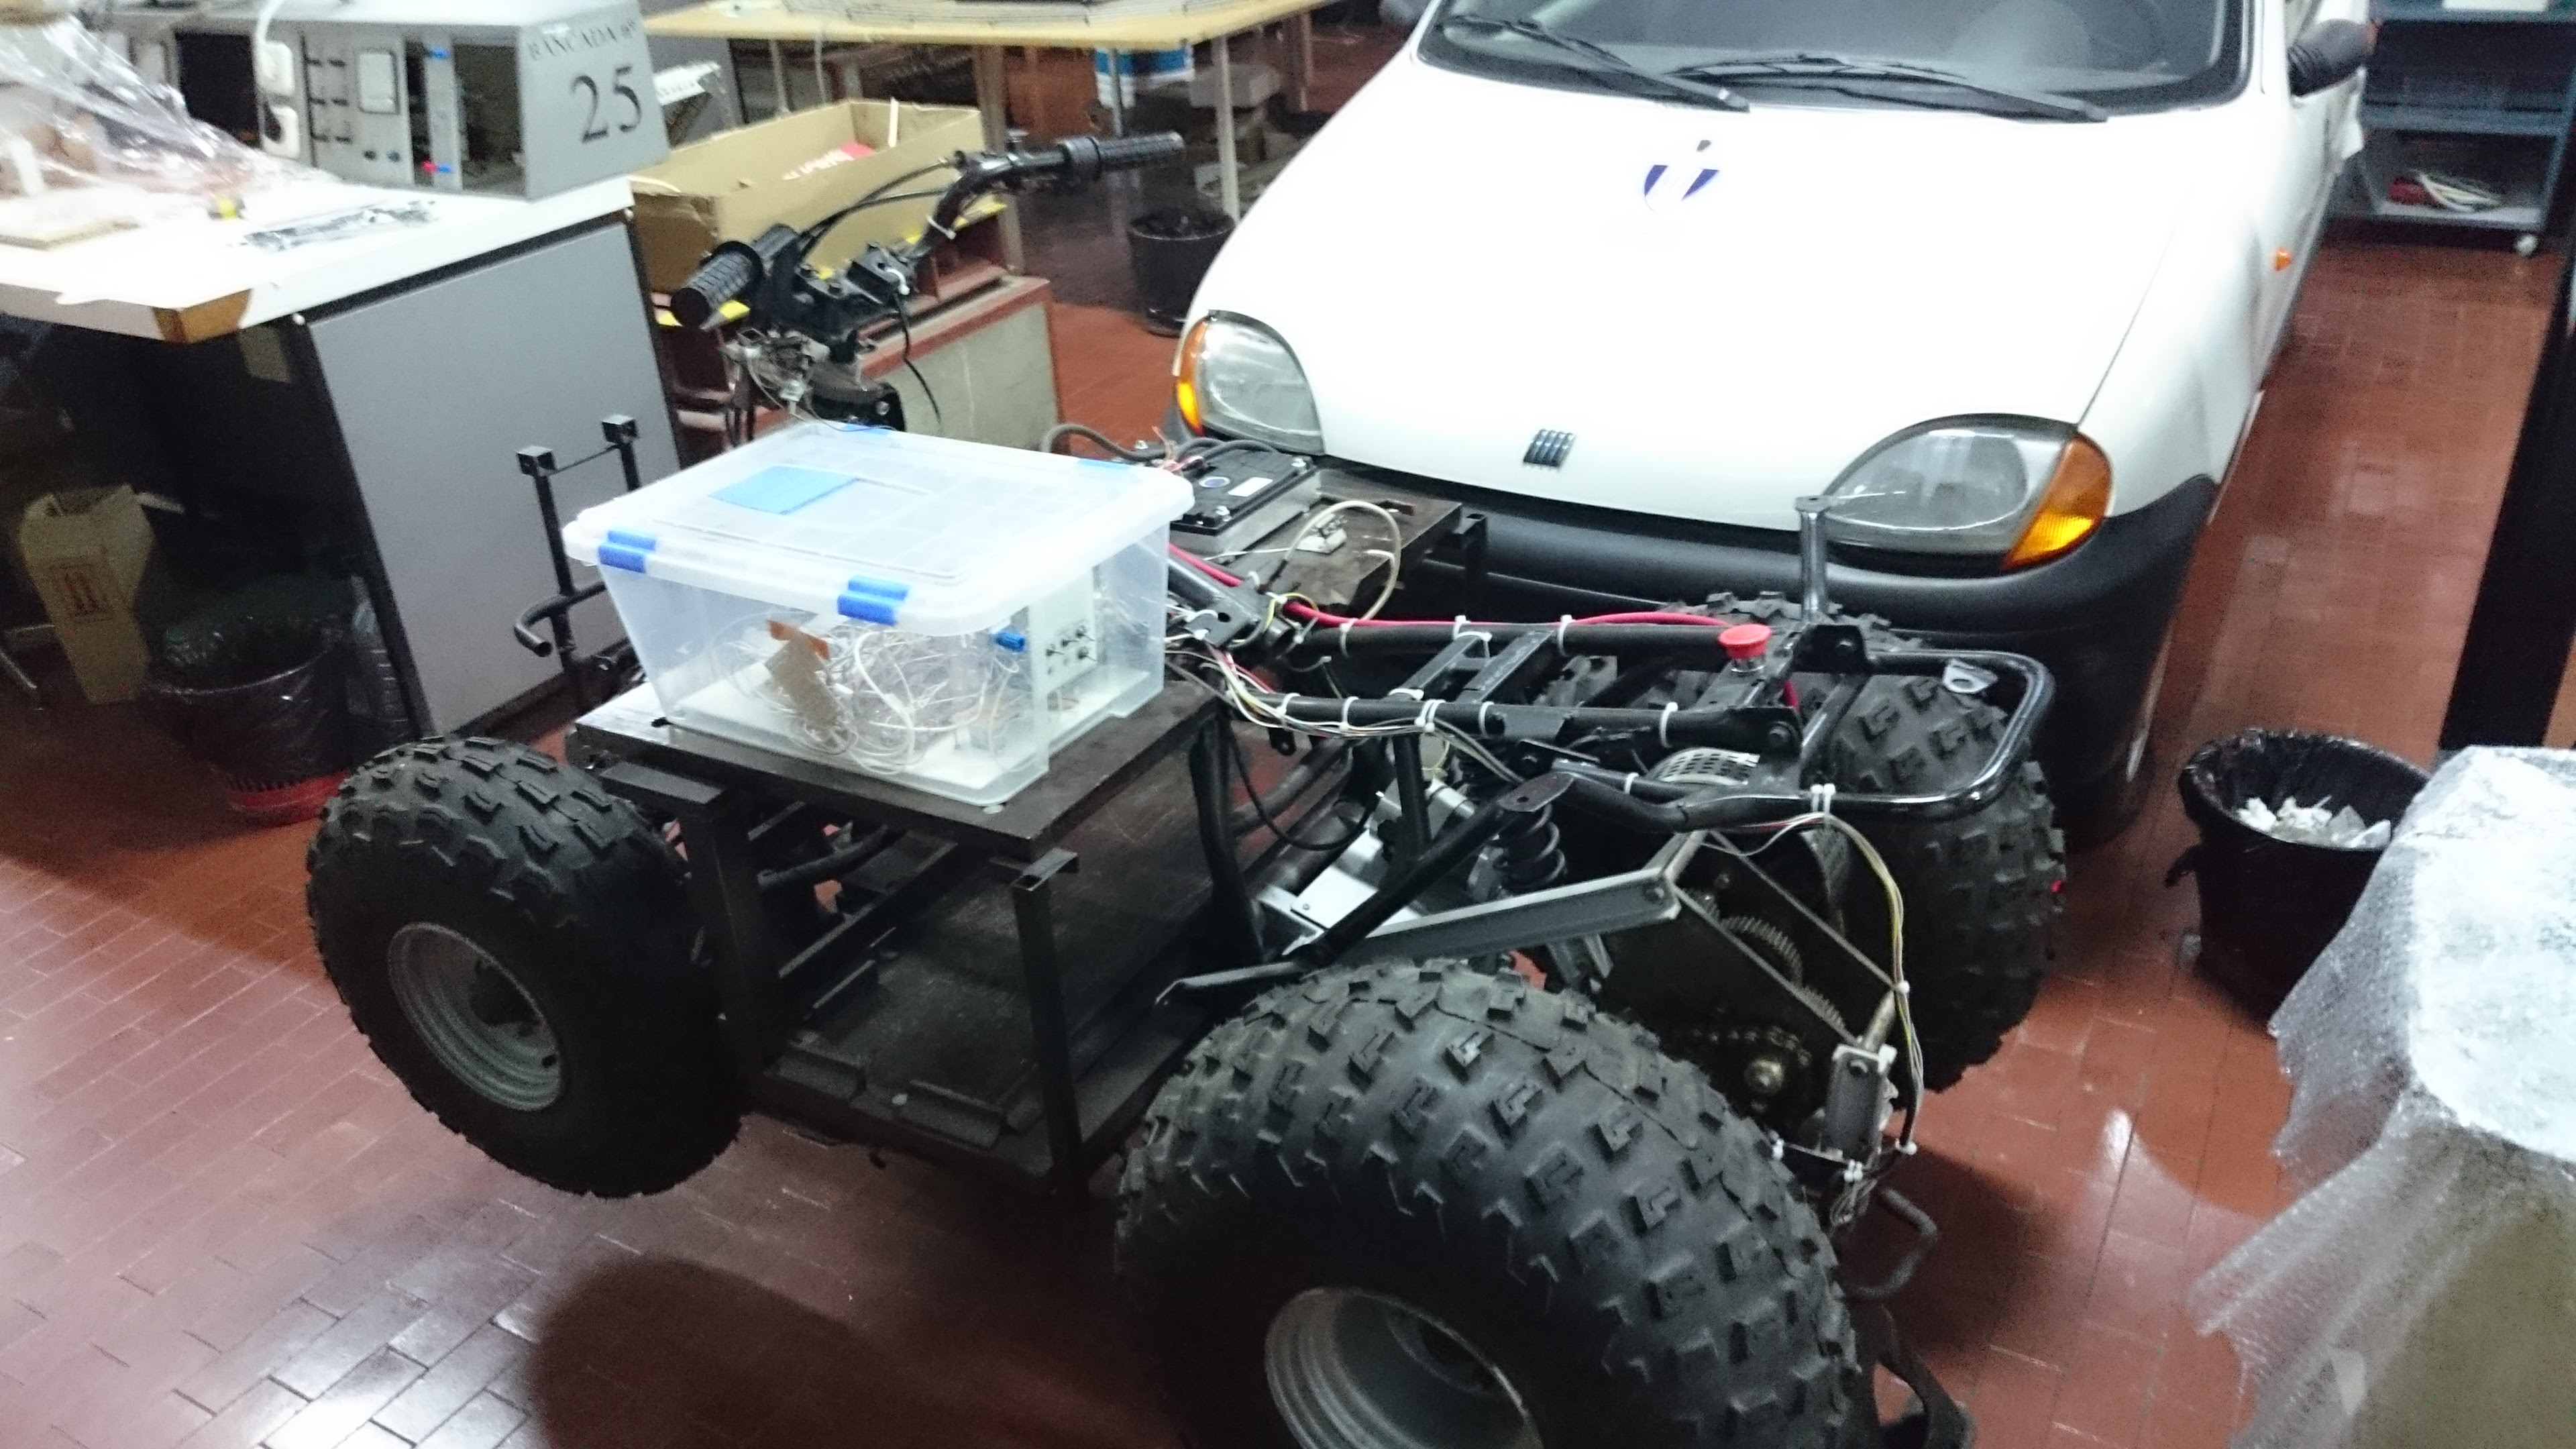
\includegraphics[height=40mm]{recursos/imagens/vista_lado_sem_baterias.jpg}  \end{center} % gr�ficos
 \vspace{5mm}
\centering
\LARGE \textbf{ROVIM T2D}
\todo{devo p�r a foto da academia militar? As regras do ist n�o preveem isso}
\todo{foto com baterias e sem carro}
\\ \vspace{10mm}
\Large Um ve�culo autonomo de vigil�ncia de instala��es militares
\\ \vspace{15mm}
\Large \textbf{Gon�alo Filipe Ribeiro Andr�}\\
\vspace{12mm}
\large Disserta��o para a obten��o do grau de mestre em
\\ \vspace{2mm}
\LARGE \textbf{Engenharia Eletrot�cnica e de Computadores}
\\ \vspace{10mm}
\large Orientadores: Prof.\todo{devi p�r Dr. tamb�m?} Ant�nio Joaquim Serralheiro\\
Prof. Duarte de Mesquita e Sousa
\\ \vspace{15mm}
\Large \textbf{J�ri}
\\ \vspace{5mm}
\large Presidente:	Prof. Lorem \\
\large Orientador: Prof. Ant�nio Joaquim Serralheiro\\
\large Co-Orientador: Prof. Duarte de Mesquita e Sousa\\
\large Vogais: Dr. Lorem Ipsum \\
Prof. Lorem Ipsum\\
 
\vspace{15mm}

%\Large \textbf{\todaythesis\today} \\
\Large \textbf{Abril 2016} \\
\let\thepage\relax
\end{flushleft}
\pagebreak


\clearpage
% Since I am using double sided pages, the second page should be white.
% Remember that when delivering the dissertation, IST requires for the cover to appear twice.

\thispagestyle{empty}
\cleardoublepage

\setcounter{page}{1} \pagenumbering{roman}

\baselineskip 18pt % line spacing: -12pt for single spacing
                   %               -18pt for 1 1/2 spacing
                   %               -24pt for double spacingnts}


\pdfbookmark{Agradecimentos}{Agradecimentos}
\begin{acknowledgments} 

Este tempo que me debrucei sobre este trabalho, foi uma �rdua jornada de desafio, constru��o e amadurecimento; nada � realizado de forma f�cil e sem esfor�o.

Quero agradecer em especial � minha fam�lia, que contribuiu para esta conquista, que me apoiou incondicionalmente e sempre acreditou em mim. Aos meus amigos e companheiros desta fase da minha vida, pelos in�meros momentos de divertimento. � minha namorada que, apesar da dist�ncia, sempre me amou e me incentivou. Ao professor Ant�nio Serralheiro, pelo suporte, corre��es e pela sua disponibilidade, porque talvez saber ensinar seja mais dif�cil que saber aprender.

\end{acknowledgments}
\clearpage
\thispagestyle{empty}
\cleardoublepage

\begin{abstract}

    In the last decade, technological advancements have enabled a rise of autonomous robotic applications for military use. With the goal of exploring its potential in surveilling military facilities, the Academia Militar commissioned the development and construction of a functioning prototype of an autonomous vehicle. In this article the traction, steering and braking actuators of such vehicle are addressed. Current research focuses on commercial road vehicle applications where autonomy is the key topic, whereas small, non-professional teams often struggle with a lack of clear vision of the whole project and lax safety procedures.
    %A quad vehicle embedded with an electric battery pack, motors, controllers and mechanical couplers to actuate its traction, steering and braking systems, along with their control and interface mechanism, with a design focus on flexibility and personnel safety is proposed and evaluated. Limitations of the proposed design are identified and solutions proposed.
    A quad vehicle embedded with an electric battery pack, traction, steering and braking actuators, along with a control and interface mechanism, with a design focus on flexibility and personnel safety is proposed and evaluated. Limitations of the proposed design are identified and solutions proposed.

\end{abstract}

\begin{keywords}
Keywords (English)
\end{keywords}
\clearpage
\thispagestyle{empty}
\cleardoublepage
\begin{resumo}

O objectivo deste trabalho ... (Portugu�s)

\end{resumo}
\begin{palavraschave}
Palavras-Chave (Portugu�s)
\end{palavraschave}
\clearpage
\thispagestyle{empty}
\cleardoublepage
% This is required for the fancy chapters
\dominitoc
\dominilof
\dominilot

%%%%%%%%%%%%%%%%%%%%%%%%%%%%%%%%%%%%%%%%%%%%%%%%%%%%%%%%%%%%%%%%%%%%%%
% List of contents
%\renewcommand{\baselinestretch}{1}
\pdfbookmark[0]{�ndice}{index}
\pdfbookmark[1]{Conte�do}{toc}
\tableofcontents
% \contentsline{chapter}{References}{\pageref{bib}}
\clearpage
\thispagestyle{empty}
\cleardoublepage
%\renewcommand{\baselinestretch}{1.5}
%%%%%%%%%%%%%%%%%%%%%%%%%%%%%%%%%%%%%%%%%%%%%%%%%%%%%%%%%%%%%%%%%%%%%%
% List of figures
\pdfbookmark[1]{Lista de Figuras}{lof}
\listoffigures
\clearpage
\thispagestyle{empty}
\cleardoublepage

%%%%%%%%%%%%%%%%%%%%%%%%%%%%%%%%%%%%%%%%%%%%%%%%%%%%%%%%%%%%%%%%%%%%%%
% List of tables
\pdfbookmark[1]{Lista de Tabelas}{lot}
\listoftables
\clearpage
\thispagestyle{empty}
\cleardoublepage

% %%%%%%%%%%%%%%%%%%%%%%%%%%%%%%%%%%%%%%%%%%%%%%%%%%%%%%%%%%%%%%%%%%%%%%
% % List of algorithms
% Requires packages algorithmic, algorithm
% \pdfbookmark[1]{List of Algorithms}{loa}
% \listofalgorithms
% \cleardoublepage

\acresetall     %faz reset as extensoes de acronimos
% %%%%%%%%%%%%%%%%%%%%%%%%%%%%%%%%%%%%%%%%%%%%%%%%%%%%%%%%%%%%%%%%%%%%%%
 % List of acronyms
\pdfbookmark[1]{Lista de Siglas e Acr�nimos}{loac}

\chapter*{Siglas, Acr�nimos e Abreviaturas}
\label{loac}


% See more at http://staff.science.uva.nl/~polko/HOWTO/LATEX/acronym.html

\todo{Como escrever o acronimo ROVIM}
\begin{acronym}
    \acro{PWM}{\emph{Pulse Width Modulation}\acroextra{, modula��o por largura de pulso}}
    \acro{ROVIM}{Rob� de Vigil�ncia de Instala��es Militares}
    \acro{T2D}{Tra��o, Travagem e Dire��o}
    \acro{SeN}{Sensores e Navega��o}
    \acro{CPC}{Comunica��es e Posto de Controlo}
    \acro{I2C}[I\textsuperscript{2}C]{\emph{Inter-Integrated Circuit}}
    \acro{OSI}{\emph{Open Systems Interconnection}}
    \acro{MDF}{\emph{Medium-Density Fibreboard}\acroextra{, fibra de madeira de m�dia densidade}}
    \acro{DC}{\emph{Direct Current}\acroextra{, corrente cont�nua}}
    \acro{AC}{\emph{Alternating Current}\acroextra{, corrente alternada}}
    \acro{rpm}{rota��es por minuto}
    \acro{NTC}{\emph{Negative Temperature Coefficient}\acroextra{, coeficiente negativo de temperatura}}
    \acro{PTC}{\emph{Positive Temperature Coefficient}\acroextra{, coeficiente positivo de temperatura}}
    \acro{NiMH}{\emph{Nickel Metal Hydride}\acroextra{, n�quel-hidreto metal}}
    \acro{VRLA}{\emph{Valve-Regulated Lead-Acid}\acroextra{, bateria de �cido chumbo selada}}
    \acro{Li-Ion}{\emph{Lithium-ion}\acroextra{, i�es de l�tio}}
    \acro{LED}{\emph{Light Emitting Diode}\acroextra{, d�odo emissor de luz}}
    \acro{FST}{Formula Student T�cnico}
    \acro{PID}{Proporcional Integral Derivativo}
    \acro{PD}{Proporcional Derivativo}
    \acro{uC}[$\mu{}$C]{Micro Controlador}
    \acro{GPIO}{\emph{General Purpose Input/Output}\acroextra{, pino program�vel de entrada/sa�da}}
    \acro{USB}{\emph{Universal Serial Bus}}
    \acro{ASCII}{\emph{American Standard Code for Information Interchange}}
    \acro{PC}{\emph{Personal Computer}\acroextra{, computador pessoal}}
    \acro{TE}{\emph{Terminal Emulator}\acroextra{, emulador de terminal}}
    \acro{TJB}{Trans�stor de Jun��o Bipolar}
    \acroplural{TJB}[TJBs]{Trans�stores de Jun��o Bipolar}
    \acro{RR}{Rela��o de Redu��o}
    %\acro{CD}{Compact Disc}
    \acro{SLIT}{Sistema Linear e Invariante no Tempo}
    \acroplural{SLIT}[SLITs]{Sistemas Lineares e Invariantes no Tempo}
    \acro{PVC}{Policloreto de Vinil}
    \acro{SMD}{\emph{Surface Mount Device}\acroextra{, dispositivo de montagem superficial}}
    \acro{PCB}{\emph{Printed Circuit Board}\acroextra{, placa de circuito impresso}}
    \acro{SPST}{\emph{Single Pole Single Throw}\acroextra{, unipolar de curso simples}}
    \acro{DPDT}{\emph{Double Pole Double Throw}\acroextra{, bipolar de curso duplo}}
    \acro{SP3T}{\emph{Single Pole Triple Throw}\acroextra{, unipolar de curso triplo}}
    \acro{ADC}{\emph{Analogue to Digital Converter}\acroextra{, conversor anal�gico--digital}}
\end{acronym}

\clearpage
\thispagestyle{empty}
\cleardoublepage




%%%%%%%%%%%%%%%%%%%%%%%%%%%%%%%%%%%%%%%%%%%%%%%%%%%%%%%%%%%%%%%%%%%%%%%
% List of symbols
\pdfbookmark[1]{Lista de S�mbolos}{los}

\listofsymbols

\clearpage
\thispagestyle{empty}

\cleardoublepage
\baselineskip 18pt

% Pages number is starting now with arabic style... until now it was on roman mode
\pagenumbering{arabic} \setcounter{page}{1}
%\pagestyle{document}%Fancy head and foot with lines
\pagestyle{documentsimple}      %Simple head
% %%%%%%%%%%%%%%%%%%%%%%%%%%%%%%%%%%%%%%%%%%%%%%%%%%%%%%%%%%%%%%%%%%%%%%
% Dummy Chapter:
% %%%%%%%%%%%%%%%%%%%%%%%%%%%%%%%%%%%%%%%%%%%%%%%%%%%%%%%%%%%%%%%%%%%%%%

% %%%%%%%%%%%%%%%%%%%%%%%%%%%%%%%%%%%%%%%%%%%%%%%%%%%%%%%%%%%%%%%%%%%%%%
% 
% %%%%%%%%%%%%%%%%%%%%%%%%%%%%%%%%%%%%%%%%%%%%%%%%%%%%%%%%%%%%%%%%%%%%%%


\section{Introdu\c{c}\~ao}
\label{sec:introducao}
Bem-vindo ao manual do utilizador do \done\todo{registar acronimos}\ac{ROVIM} \ac{T2D}.\\
O \ac{ROVIM} � uma plataforma m�vel de vigil�ncia de instala��es militares. � baseado num \emph{chassis} de moto-quatro equipado de motores el�ctricos para trac��o, travagem e de direc��o. Esta plataforma est� equipada com sensores diversos e com m�dulos de comunica��o via r�dio com uma esta��o de controlo.\\
O \ac{ROVIM} � consistindo por 3 subsistemas ou m�dulos: \ac{T2D}, \ac{SeN} e \ac{CPC}, cujas funcionalidades se complementam e conjugam de acordo com um modelo em camadas, semelhante ao modelo \ac{OSI}.\\
O m�dulo \ac{T2D} corresponde � camada de mais baixo n�vel, e consiste dos motores e seus controladores, baterias e sistemas de monitoriza��o e controlo embarcados no \emph{chassis} do ve�culo. � o m�dulo \ac{T2D} que permite a movimenta��o da plataforma, atrav�s de comandos recebidos do m�dulo \ac{SeN}. O \ac{T2D} foi concebido para tamb�m poder ser operado de forma manual, controlado localmente por um utilizador humano.\\
Este manual descreve o m�dulo \ac{T2D} do ponto de vista do utilizador final, focando-se nos aspetos funcionais em detrimento dos detalhes de implementa��o. Destina-se a todos os utilizadores da plataforma \ac{ROVIM}, e pretende servir de manual de aprendizagem r�pida e guia de campo.\\
Este documento pretende tamb�m oferecer informa��o coerente, j� que � atualizado em conjunto com a plataforma, ao contr�rio de outra documenta��o, como teses de mestrado.\\
� recomendada a leitura completa deste manual antes de operar o rob� pela primeira vez e a sua consulta para esclarecimento de d�vidas durante a utiliza��o do ve�culo.\\
� apresentada inicialmente uma vis�o geral resumida do m�dulo, para familiarizar os leitores. Seguem-se instru��es detalhadas sobre o manuseamento e condu��o do ve�culo. Por fim apresenta-se um guia sobre modifica��es e reconfigura��es do sistema.\\
Neste documento os termos \ac{ROVIM}, \ac{T2D}, m�dulo, plataforma, moto, rob� e ve�culo ser�o usados indistintamente.


\section{Obter ajuda}
\label{sec:ajuda}
A utiliza��o do \ac{ROVIM} pode suscitar d�vidas a alguns utilizadores mais inexperientes. Existem no entanto v�rias formas de obter ajuda e esclarecer d�vidas ao seu dispor:
\begin{itemize}
    \item \textbf{Este manual.} Aqui s�o esclarecidas a maior parte das d�vidas que podem surgir na utiliza��o do ve�culo. Cont�m informa��o mais atualizada que as teses de mestrado.
    \item \textbf{Documenta��o produzida pelos anteriores colaboradores.} Esta deve conter detalhes sobre o c�digo fonte, esquemas el�tricos e \emph{layout} dos componentes eletr�nicos, entre outra informa��o. Esta documenta��o � de livre acesso, mas pode ser obtida junto dos colaboradores do projeto.
    \item \textbf{Documenta��o dos v�rios componentes individuais.} Muita desta documenta��o est� livremente acess�vel na internet, mas pode ser obtida junto dos colaboradores do projeto. A lista de componentes est� dispon�vel no \nameref{ap:c}.
    \item \textbf{Reposit�rio do c�digo do projeto,} em \url{https://github.com/ROVIM-T2D/ROVIM-T2D-Brain.git}. O c�digo aqui encontrado pode ser mais recente que o c�digo programado no ve�culo.
    \item \textbf{Os \nameref{sec:colaboradores} do projecto}. Os antigos e atuais colaboradores estar�o dispon�veis para ajudar a esclarecer d�vidas e aconselhar os atuais colaboradores e utilizadores.
\end{itemize}


\section{Considera\c{c}\~oes de seguran\c{c}a}
\label{sec:seguranca}
O ROVIM foi projectado com um �nfase na seguran�a dos utilizadores. A�nda ssim, � um prot�tipo insuficientemente refinado e testado para poder ser usado em condi��es desfavor�veis, ou por utilizadores inexperientes ou impreparados. Esta fragilidade aliada ao peso e pot�ncia do rob�t tornam a sua utiliza��o pot�ncialmente perigosa. Este cap�tulo imp�e aos utilizadores normas que devem ser seguidas constantemente e impreter�velmente para min�mizar os riscos e a gravidade de pot�nciais acidentes.
\begin{comment}
    rascunho das normas:
    -operar em terreno pouco acidentado
    -operar sem chuva
    -manter a frente do ve�culo sempre desimpedida de obst�culos
    -projectar a trajectoria pretendida para o ve�culo antes de o ligar, e garantir que esta se encontra desimpedida de pessoas ou outros obst�culos
    -alertar as pessoas na vizinha�a do ve�culo para o facto de este estar a ser utilizado e os seus perigos
    -l�r e compreender este manual antes de operar o ve�culo pela primeira vez
    -levantar as rodas de tr�s do ch�o quando o desligar
    -aprender a operar o veiculo com as 4 rodas no ar, antes de passar para o ch�o. Familiazirar-se com todas as funcionalidades e procedimentos de seguran�a
    -Manter sempre o dispositivo do homem-morto pronto a disparar (de prefer�ncia atado ao bra�o do utilizador)
\end{comment}
\\


\section{Descri��o do sistema}
\label{sec:descricao_sistema}

\subsection{\emph{Hardware}}
\label{ssec:descricao_hardware}
\subsubsection{Tra��o}
\label{sssec:tracao}
\subsubsection{Travagem}
\label{sssec:travagem}
\subsubsection{Dire��o}
\label{sssec:direcao}
\subsubsection{Energia}
\label{sssec:energia}
\subsubsection{Controlo}
\label{sssec:controlo}

\subsection{\emph{Software}}
\label{ssec:descricao_software}
\subsubsection{Arquitetura}
\label{sssec:arquitetura}


\section{Interface com o utilizador}
\label{sec:interface}
%analisar melhor como fazer aqui com os bot�es/controlos. � que os controlos s�o uma constru��o sobre a interface. Os but�es � que constituem a dita.


\section{Estados do sistema}
\label{sec:estados}


\subsection{Modo manual}
\label{ssec:estados_manual}



\subsection{Modo autom�tico}
\label{ssec:estados_auto}




\section{Funcionalidades}
\label{sec:funcionalidades}

-ligar\\
-desligar\\
-ir para lockdown\\
-sair de lockdown\\
-entrar em modo manual\\
-ponto morto\\
-hillhold\\
-acelerar\\
-desacelerar\\

\subsection{Modo autom�tico}
\label{ssec:funcionalidades_automatico}
\subsubsection{Interace TE}
\label{sssec:interface_te}
\label{auto:desligar}
\subsubsection{Interface I2C}
\label{sssec:interface_i2c}
N/A por enquanto.
\subsubsection{Interface R/C}
\label{sssec:interface_rc}
N/A



\subsection{Modo manual}
\label{ssec:funcionalidades_manual}




\section{Manuten\c{c}\~ao e transporte}
\label{manutencao}


\section{Resolu��o de problemas}
\label{sec:resolucao_problemas}
-lista erros SigmaD\\
-reinicio dalf ocasionalmente aquando da trv/destrv emerg.\\
-funcionalidades debug\\
-o que fazer num erro desconhecido\\

\section{Problemas conhecidos}
\label{sec:problemas_conhecidos}
-a velocidade mt baixa <~1 km/h a leitura do sensor n�o tem exatid�o.

%\input{conteudo/}
\cleardoublepage


%this is just here temporarily, to have references for the biblio
%% %%%%%%%%%%%%%%%%%%%%%%%%%%%%%%%%%%%%%%%%%%%%%%%%%%%%%%%%%%%%%%%%%%%%%%
% Dummy Chapter:
% %%%%%%%%%%%%%%%%%%%%%%%%%%%%%%%%%%%%%%%%%%%%%%%%%%%%%%%%%%%%%%%%%%%%%%

% %%%%%%%%%%%%%%%%%%%%%%%%%%%%%%%%%%%%%%%%%%%%%%%%%%%%%%%%%%%%%%%%%%%%%%
% 
% %%%%%%%%%%%%%%%%%%%%%%%%%%%%%%%%%%%%%%%%%%%%%%%%%%%%%%%%%%%%%%%%%%%%%%


\section{Introdu\c{c}\~ao}
\label{sec:introducao}
Bem-vindo ao manual do utilizador do \done\todo{registar acronimos}\ac{ROVIM} \ac{T2D}.\\
O \ac{ROVIM} � uma plataforma m�vel de vigil�ncia de instala��es militares. � baseado num \emph{chassis} de moto-quatro equipado de motores el�ctricos para trac��o, travagem e de direc��o. Esta plataforma est� equipada com sensores diversos e com m�dulos de comunica��o via r�dio com uma esta��o de controlo.\\
O \ac{ROVIM} � consistindo por 3 subsistemas ou m�dulos: \ac{T2D}, \ac{SeN} e \ac{CPC}, cujas funcionalidades se complementam e conjugam de acordo com um modelo em camadas, semelhante ao modelo \ac{OSI}.\\
O m�dulo \ac{T2D} corresponde � camada de mais baixo n�vel, e consiste dos motores e seus controladores, baterias e sistemas de monitoriza��o e controlo embarcados no \emph{chassis} do ve�culo. � o m�dulo \ac{T2D} que permite a movimenta��o da plataforma, atrav�s de comandos recebidos do m�dulo \ac{SeN}. O \ac{T2D} foi concebido para tamb�m poder ser operado de forma manual, controlado localmente por um utilizador humano.\\
Este manual descreve o m�dulo \ac{T2D} do ponto de vista do utilizador final, focando-se nos aspetos funcionais em detrimento dos detalhes de implementa��o. Destina-se a todos os utilizadores da plataforma \ac{ROVIM}, e pretende servir de manual de aprendizagem r�pida e guia de campo.\\
Este documento pretende tamb�m oferecer informa��o coerente, j� que � atualizado em conjunto com a plataforma, ao contr�rio de outra documenta��o, como teses de mestrado.\\
� recomendada a leitura completa deste manual antes de operar o rob� pela primeira vez e a sua consulta para esclarecimento de d�vidas durante a utiliza��o do ve�culo.\\
� apresentada inicialmente uma vis�o geral resumida do m�dulo, para familiarizar os leitores. Seguem-se instru��es detalhadas sobre o manuseamento e condu��o do ve�culo. Por fim apresenta-se um guia sobre modifica��es e reconfigura��es do sistema.\\
Neste documento os termos \ac{ROVIM}, \ac{T2D}, m�dulo, plataforma, moto, rob� e ve�culo ser�o usados indistintamente.


\section{Obter ajuda}
\label{sec:ajuda}
A utiliza��o do \ac{ROVIM} pode suscitar d�vidas a alguns utilizadores mais inexperientes. Existem no entanto v�rias formas de obter ajuda e esclarecer d�vidas ao seu dispor:
\begin{itemize}
    \item \textbf{Este manual.} Aqui s�o esclarecidas a maior parte das d�vidas que podem surgir na utiliza��o do ve�culo. Cont�m informa��o mais atualizada que as teses de mestrado.
    \item \textbf{Documenta��o produzida pelos anteriores colaboradores.} Esta deve conter detalhes sobre o c�digo fonte, esquemas el�tricos e \emph{layout} dos componentes eletr�nicos, entre outra informa��o. Esta documenta��o � de livre acesso, mas pode ser obtida junto dos colaboradores do projeto.
    \item \textbf{Documenta��o dos v�rios componentes individuais.} Muita desta documenta��o est� livremente acess�vel na internet, mas pode ser obtida junto dos colaboradores do projeto. A lista de componentes est� dispon�vel no \nameref{ap:c}.
    \item \textbf{Reposit�rio do c�digo do projeto,} em \url{https://github.com/ROVIM-T2D/ROVIM-T2D-Brain.git}. O c�digo aqui encontrado pode ser mais recente que o c�digo programado no ve�culo.
    \item \textbf{Os \nameref{sec:colaboradores} do projecto}. Os antigos e atuais colaboradores estar�o dispon�veis para ajudar a esclarecer d�vidas e aconselhar os atuais colaboradores e utilizadores.
\end{itemize}


\section{Considera\c{c}\~oes de seguran\c{c}a}
\label{sec:seguranca}
O ROVIM foi projectado com um �nfase na seguran�a dos utilizadores. A�nda ssim, � um prot�tipo insuficientemente refinado e testado para poder ser usado em condi��es desfavor�veis, ou por utilizadores inexperientes ou impreparados. Esta fragilidade aliada ao peso e pot�ncia do rob�t tornam a sua utiliza��o pot�ncialmente perigosa. Este cap�tulo imp�e aos utilizadores normas que devem ser seguidas constantemente e impreter�velmente para min�mizar os riscos e a gravidade de pot�nciais acidentes.
\begin{comment}
    rascunho das normas:
    -operar em terreno pouco acidentado
    -operar sem chuva
    -manter a frente do ve�culo sempre desimpedida de obst�culos
    -projectar a trajectoria pretendida para o ve�culo antes de o ligar, e garantir que esta se encontra desimpedida de pessoas ou outros obst�culos
    -alertar as pessoas na vizinha�a do ve�culo para o facto de este estar a ser utilizado e os seus perigos
    -l�r e compreender este manual antes de operar o ve�culo pela primeira vez
    -levantar as rodas de tr�s do ch�o quando o desligar
    -aprender a operar o veiculo com as 4 rodas no ar, antes de passar para o ch�o. Familiazirar-se com todas as funcionalidades e procedimentos de seguran�a
    -Manter sempre o dispositivo do homem-morto pronto a disparar (de prefer�ncia atado ao bra�o do utilizador)
\end{comment}
\\


\section{Descri��o do sistema}
\label{sec:descricao_sistema}

\subsection{\emph{Hardware}}
\label{ssec:descricao_hardware}
\subsubsection{Tra��o}
\label{sssec:tracao}
\subsubsection{Travagem}
\label{sssec:travagem}
\subsubsection{Dire��o}
\label{sssec:direcao}
\subsubsection{Energia}
\label{sssec:energia}
\subsubsection{Controlo}
\label{sssec:controlo}

\subsection{\emph{Software}}
\label{ssec:descricao_software}
\subsubsection{Arquitetura}
\label{sssec:arquitetura}


\section{Interface com o utilizador}
\label{sec:interface}
%analisar melhor como fazer aqui com os bot�es/controlos. � que os controlos s�o uma constru��o sobre a interface. Os but�es � que constituem a dita.


\section{Estados do sistema}
\label{sec:estados}


\subsection{Modo manual}
\label{ssec:estados_manual}



\subsection{Modo autom�tico}
\label{ssec:estados_auto}




\section{Funcionalidades}
\label{sec:funcionalidades}

-ligar\\
-desligar\\
-ir para lockdown\\
-sair de lockdown\\
-entrar em modo manual\\
-ponto morto\\
-hillhold\\
-acelerar\\
-desacelerar\\

\subsection{Modo autom�tico}
\label{ssec:funcionalidades_automatico}
\subsubsection{Interace TE}
\label{sssec:interface_te}
\label{auto:desligar}
\subsubsection{Interface I2C}
\label{sssec:interface_i2c}
N/A por enquanto.
\subsubsection{Interface R/C}
\label{sssec:interface_rc}
N/A



\subsection{Modo manual}
\label{ssec:funcionalidades_manual}




\section{Manuten\c{c}\~ao e transporte}
\label{manutencao}


\section{Resolu��o de problemas}
\label{sec:resolucao_problemas}
-lista erros SigmaD\\
-reinicio dalf ocasionalmente aquando da trv/destrv emerg.\\
-funcionalidades debug\\
-o que fazer num erro desconhecido\\

\section{Problemas conhecidos}
\label{sec:problemas_conhecidos}
-a velocidade mt baixa <~1 km/h a leitura do sensor n�o tem exatid�o.

%\input{conteudo/}
\cleardoublepage



\cleardoublepage
\phantomsection     %http://tex.stackexchange.com/questions/44088/when-do-i-need-to-invoke-phantomsection
\addcontentsline{toc}{chapter}{Bibliografia}    %Add bibliography to toc
%http://tex.stackexchange.com/questions/17128/using-bibtex-to-make-a-list-of-references-without-having-citations-in-the-body-of
\nocite{*}      %show bibliography even if there are no citations
\bibliographystyle{IEEEtran}
\bibliography{recursos/biblio}
\todo{colocar bibliografia em portugues}
\cleardoublepage


\begin{appendices}
	\begin{appendix}
		\pagenumbering{bychapter}
		
\fancychapter{Ap�ndice A - c�digo do programa}
\label{ap:a}

\lstset{ %
language=[ANSI]C,                % choose the language of the code
basicstyle=\footnotesize,       % the size of the fonts that are used for the code
numbers=left,                   % where to put the line-numbers
numberstyle=\footnotesize,      % the size of the fonts that are used for the line-numbers
stepnumber=1,                   % the step between two line-numbers. If it is 1 each line will be numbered
numbersep=5pt,                  % how far the line-numbers are from the code
backgroundcolor=\color{white},  % choose the background color. You must add \usepackage{color}
showspaces=false,               % show spaces adding particular underscores
showstringspaces=false,         % underline spaces within strings
showtabs=false,                 % show tabs within strings adding particular underscores
frame=single,           % adds a frame around the code
%tabsize=2,          % sets default tabsize to 2 spaces
captionpos=b,           % sets the caption-position to bottom
breaklines=true,        % sets automatic line breaking
breakatwhitespace=false    % sets if automatic breaks should only happen at whitespace
%escapeinside={\%*}{*)}          % if you want to add a comment within your code
}

O c�digo fonte usado na programa��o da placa de controlo da \ac{T2D} � demasiado extenso para ser aqui listado, pelo que � fornecido num ficheiro complementar a esta disserta��o. Uma c�pia exata destes ficheiros, assim como outros ficheiros usados no projeto est� acess�vel em: \url{https://github.com/ROVIM-T2D/ROVIM-T2D-Brain/tree/\swversion}.

Os ficheiros \verb!main.c! e \verb!dalf.h! s�o altera��es aos ficheiros originais fornecidos com a placa Dalf para esta aplica��o, e s�o licenciados pela \emph{Embedded Electronics, LLC}\@.

A biblioteca \verb!dalf.lib! � tamb�m necess�ria para gerar o programa, mas n�o � listada aqui por n�o ter sido alterada da vers�o original, por estar em formato bin�rio, e por regras de licenciamento restritas. A licen�a destes ficheiros pode ser consultada no site do fornecedor, em: \url{http://www.embeddedelectronics.net/documents/Ver160/EULA.pdf}.

\done\todo{mostrar restantes ficheiros de c�digo}

\done\todo[Fix]{a listagem do c�digo ocupa atualmente ~70 p�ginas}

Os ficheiros listados no ficheiro s�o:

\begin{itemize}
    \item \verb!main.c!
    \item \verb!dalf_ext.c!
    \item \verb!dalf.h!
    \item \verb!config.h!
    \item \verb!p18f6722.h!
    \item \verb!rovim_t2d.c!
    \item \verb!rovim_t2d.h!
    \item \verb!rovim.h!
    \item \verb!rovim_config_t2d_development.h!
\end{itemize}

%\lstinputlisting{recursos/codigo/\swversion/main.c}
%\lstinputlisting{recursos/codigo/\swversion/dalf_ext.c}
%\lstinputlisting{recursos/codigo/\swversion/dalf.h}
%\lstinputlisting{recursos/codigo/\swversion/config.h}
%\lstinputlisting{recursos/codigo/\swversion/p18f6722.h}
%\lstinputlisting{recursos/codigo/\swversion/rovim_t2d.c}
%\lstinputlisting{recursos/codigo/\swversion/rovim_t2d.h}
%\lstinputlisting{recursos/codigo/\swversion/rovim.h}
%\lstinputlisting{recursos/codigo/\swversion/rovim_config_t2d_development.h}

\cleardoublepage
   
        
\fancychapter{Ap�ndice B - Esquemas el�tricos e \emph{layout} das placas eletr�nicas}
\label{ap:b}


\cleardoublepage

        \fancychapter{Ap�ndice C - Lista de componentes}
\label{ap:c}

%\begin{table}
%\begin{center}
%\begin{longtable}{ @{} m{0.05\textwidth} m{0.18\textwidth} m{0.6\textwidth} m{0.1\textwidth} @{} }
\begin{row_labeled_longtable}{Componentes}{ m{0.05\textwidth} m{0.05\textwidth} m{0.18\textwidth} m{0.6\textwidth} m{0.1\textwidth}} {C}
    \toprule
    %the multicolum supresses the rule for the automatic component count of this environment. See: http://tex.stackexchange.com/questions/120648/changing-the-table-row-height-in-all-rows-except-the-first-row?rq=1
    %Bug: Idk how to supress left border space in the multicolumn - so it disaligns with the rest of column - bummer
    \multicolumn{1}{ l }{Id.\footnote{Identifica��o}} & Qt.\footnote{Quantidade} & Componente & Descri��o & Subsistema\footnote{Pe�a a que o componente pertence, se aplic�vel}\\
    \midrule
    & 1 & \emph{Chassis} & \emph{Chassis}, rodas, eixo traseiro com carreto de transmiss�o e sistemas de travagem e viragem de moto-quatro & \emph{Chassis}\\
    & Indef.\footnote{Quantidade indefinida} & Ferro sortido & Ferro usado nas estruturas de fixa��o de componentes\footnote{Que s�o: 1) Estrutura central de fixa��o das plataformas; 2) estrutura de suporte do redutor de dire��o; 3) estrutura de fixa��o do motor de tra��o; 4) estrutura de fixa��o do sensor de velocidade} e outras adapta��es soldadas ao \emph{chassis} & \emph{Chassis}\\
    %In. & Parafusos & Parafusos de ferro de v�rias medidas, usados na fixa��o dos componentes ao \emph{chassis} & \emph{Chassis}\\
    %In. & Anilhas & Anilhas de ferro de v�rias medidas, usadas na fixa��o dos componentes ao \emph{chassis} & \emph{Chassis}\\
    %In. & Porcas & Porcas de ferro de v�rias medidas, usadas na fixa��o dos componentes ao \emph{chassis} & \emph{Chassis}\\
    & Indef. & Material de fixa��o & Porcas, parafusos, anilhas, anilhas de mola, cavilhas e outros materiais n�o discriminados de diversas medidas, usados na fixa��o r�gida dos componentes, entre si, ou ao \emph{chassis} &\\
    & 1 & Plataforma inferior & Plataforma de madeira \ac{MDF} cortada, furada e escareada, � medida para a estrutura inferior & \emph{Chassis}\\
    & 1 & Mini-plataforma inferior & Plataforma de madeira \ac{MDF} cortada, furada e escareada, entre a estrutura inferior e a coluna da dire��o & \emph{Chassis}\\
    & 2 & T�buas de madeira & T�buas de madeira, cortadas � medida, fixadas verticalmente � parte frontal da estrutura de suporte das plataformas, para conten��o das baterias & \emph{Chassis}\\
    & 1 & Plataforma superior bombordo & Plataforma de madeira \ac{MDF} cortada, furada e escareada, � medida para o lado de bombordo da estrutura superior & \emph{Chassis}\\
    & 1 & Plataforma superior estibordo & Plataforma de madeira \ac{MDF} cortada, furada e escareada, � medida para o lado de estibordo da estrutura superior & \emph{Chassis}\\
    & 7 & Cantoneiras de madeira & Cantoneiras de madeira, de tamanhos diversos, coladas � plataforma inferior, para conten��o das baterias ao n�vel da base& \emph{chassis}\\
    & 6 & Baterias NP55-12R & Baterias recarreg�veis seladas de �cido-chumbo, de 12 V & Baterias\\
    & 4 & El�sticos de reten��o de cargas & El�sticos, de tamanhos diversos, com ganchos de ferro nas pontas, para abra�ar e conter as baterias ao n�vel do topo & \\
    & 1 & Carregador de baterias 12 V & Carregador de baterias de �cido-chumbo de 12 V &\\
    & 1 & Carregador de baterias 72 V & Carregador de baterias de �cido-chumbo de 72 V &\\
    & 1 & Agni B-95R & Motor \ac{DC} com escovas & \\
    & 1 & Carreto de 11 dentes & Carreto compat�vel com o carreto instalado no veio traseiro & Redutor da tra��o\\
    & 2 & Engrenagens 42 dentes & Engrenagens cil�ndricas, de m�dulo 2, �ngulo de press�o de 20�, material \texttt{C 43 UNI 7847}, de acordo com o cat�logo eurocorreias 2012 \cite{catalogo_eurocorreias} & Redutor da tra��o\\
    & 1 & Engrenagem 21 dentes & Engrenagens cil�ndricas, de m�dulo 2, �ngulo de press�o de 20�, material \texttt{C 43 UNI 7847}, de acordo com o cat�logo eurocorreias 2012 \cite{catalogo_eurocorreias} & Redutor da tra��o\\
    & 1 & Engrenagem 14 dentes & Engrenagens cil�ndricas, de m�dulo 2, �ngulo de press�o de 20�, material \texttt{C 43 UNI 7847}, de acordo com o cat�logo eurocorreias 2012 \cite{catalogo_eurocorreias} & Redutor da tra��o\\
    & 2 & Rolamentos \texttt{Koyo} 6001 & Rolamentos ranhurados de esferas, como especifica��o do catalogo \texttt{Koyo} \cite{catalogo_rolamentos} & Redutor da tra��o\\
    & 2 & Rolamentos \texttt{Koyo} 6003 & Rolamentos ranhurados de esferas, como especifica��o do catalogo \texttt{Koyo} \cite{catalogo_rolamentos} & Redutor da tra��o\\
    & 1 & Chave de veio & Chave para fixa��o de engrenagem ao veio do motor de tra��o, de acordo com a norma ISO/R773 \cite{norma_ISO_R773} & Redutor da tra��o\\
    %& 1 & Freio & Freio para segurar veio em posi��o\todo{confirmar} & Redutor da tra��o\\
    & 1 & Espa�ador para veio & Espa�ador para segurar engrenagem no veio do motor & Redutor da tra��o\\
    & 1 & Fixador para carreto & Bolacha com furo para fixar carreto acoplado ao redutor no veio & Redutor da tra��o\\
    & 1 & Chapa motor & Chapa estrutural de fixa��o dos componentes do redutor do motor, de acordo com o desenho "chapa motor" do ap�ndice \ref{ap:d} & Redutor da tra��o\\
    & 1 & Chapa corrente & Chapa estrutural de fixa��o dos componentes do redutor do motor, de acordo com o desenho "chapa corrente" do ap�ndice \ref{ap:d} & Redutor da tra��o\\
    & 1 & Veio 16 mm & Veio de fixa��o de engrenagens do redutor do motor, de acordo com o desenho "veio 16.12" do ap�ndice \ref{ap:d} & Redutor da tra��o\\
    & 1 & Veio 17 mm & Veio de fixa��o de engrenagens do redutor do motor, de acordo com o desenho "20.23" do ap�ndice \ref{ap:d} & Redutor da tra��o\\
    & Indef. & Material de fixa��o do redutor & Freio, parafusos, anilhas e anilhas de mola de diversas medidas usadas na fixa��o dos componentes do redutor do motor de tra��o & Redutor da tra��o\\
    & 1 & Corrente & Corrente original da moto-quatro & \\
    & 1 & Sigmadrive PMT835M & Controlador de motor \ac{DC} de �manes permanentes & \todo{lista de componentes do sensor de velocidade}\\
    \bottomrule
\end{row_labeled_longtable}
%\end{longtable}
%\end{center}
%\end{table}
\cleardoublepage

        
\fancychapter{Ap�ndice D - desenhos t�cnicos das pe�as do redutor do motor de tra��o}
\label{ap:d}

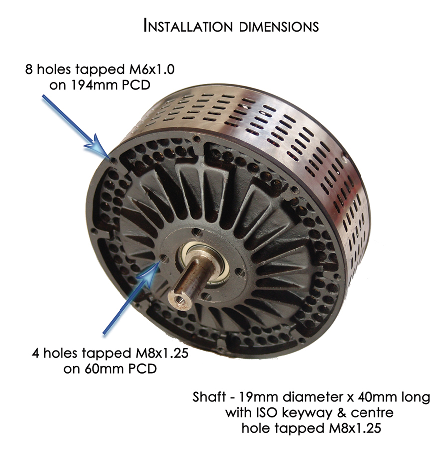
\includepdf[landscape=true]{recursos/esquemas/redutor_tracao_v1.0/motor.pdf}
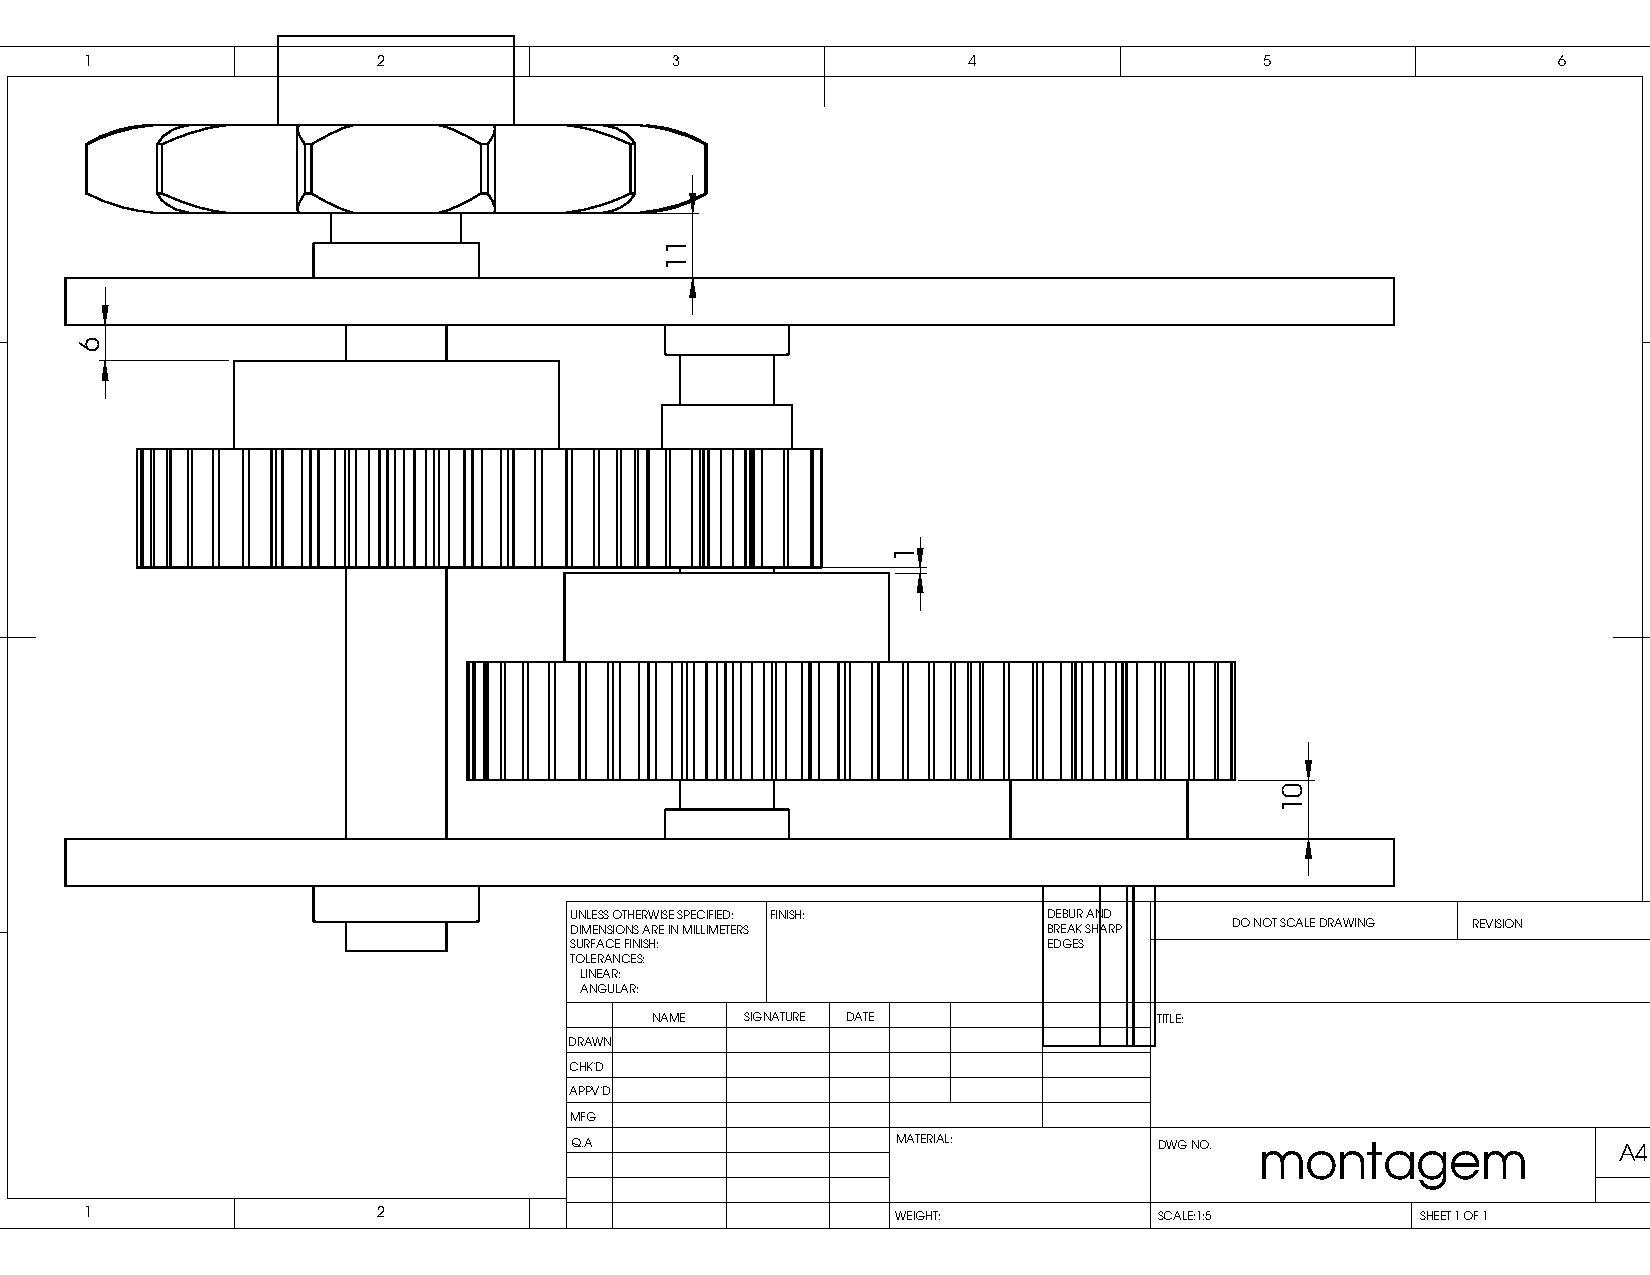
\includepdf[landscape=true]{recursos/esquemas/redutor_tracao_v1.0/montagem_vista_cima.pdf}
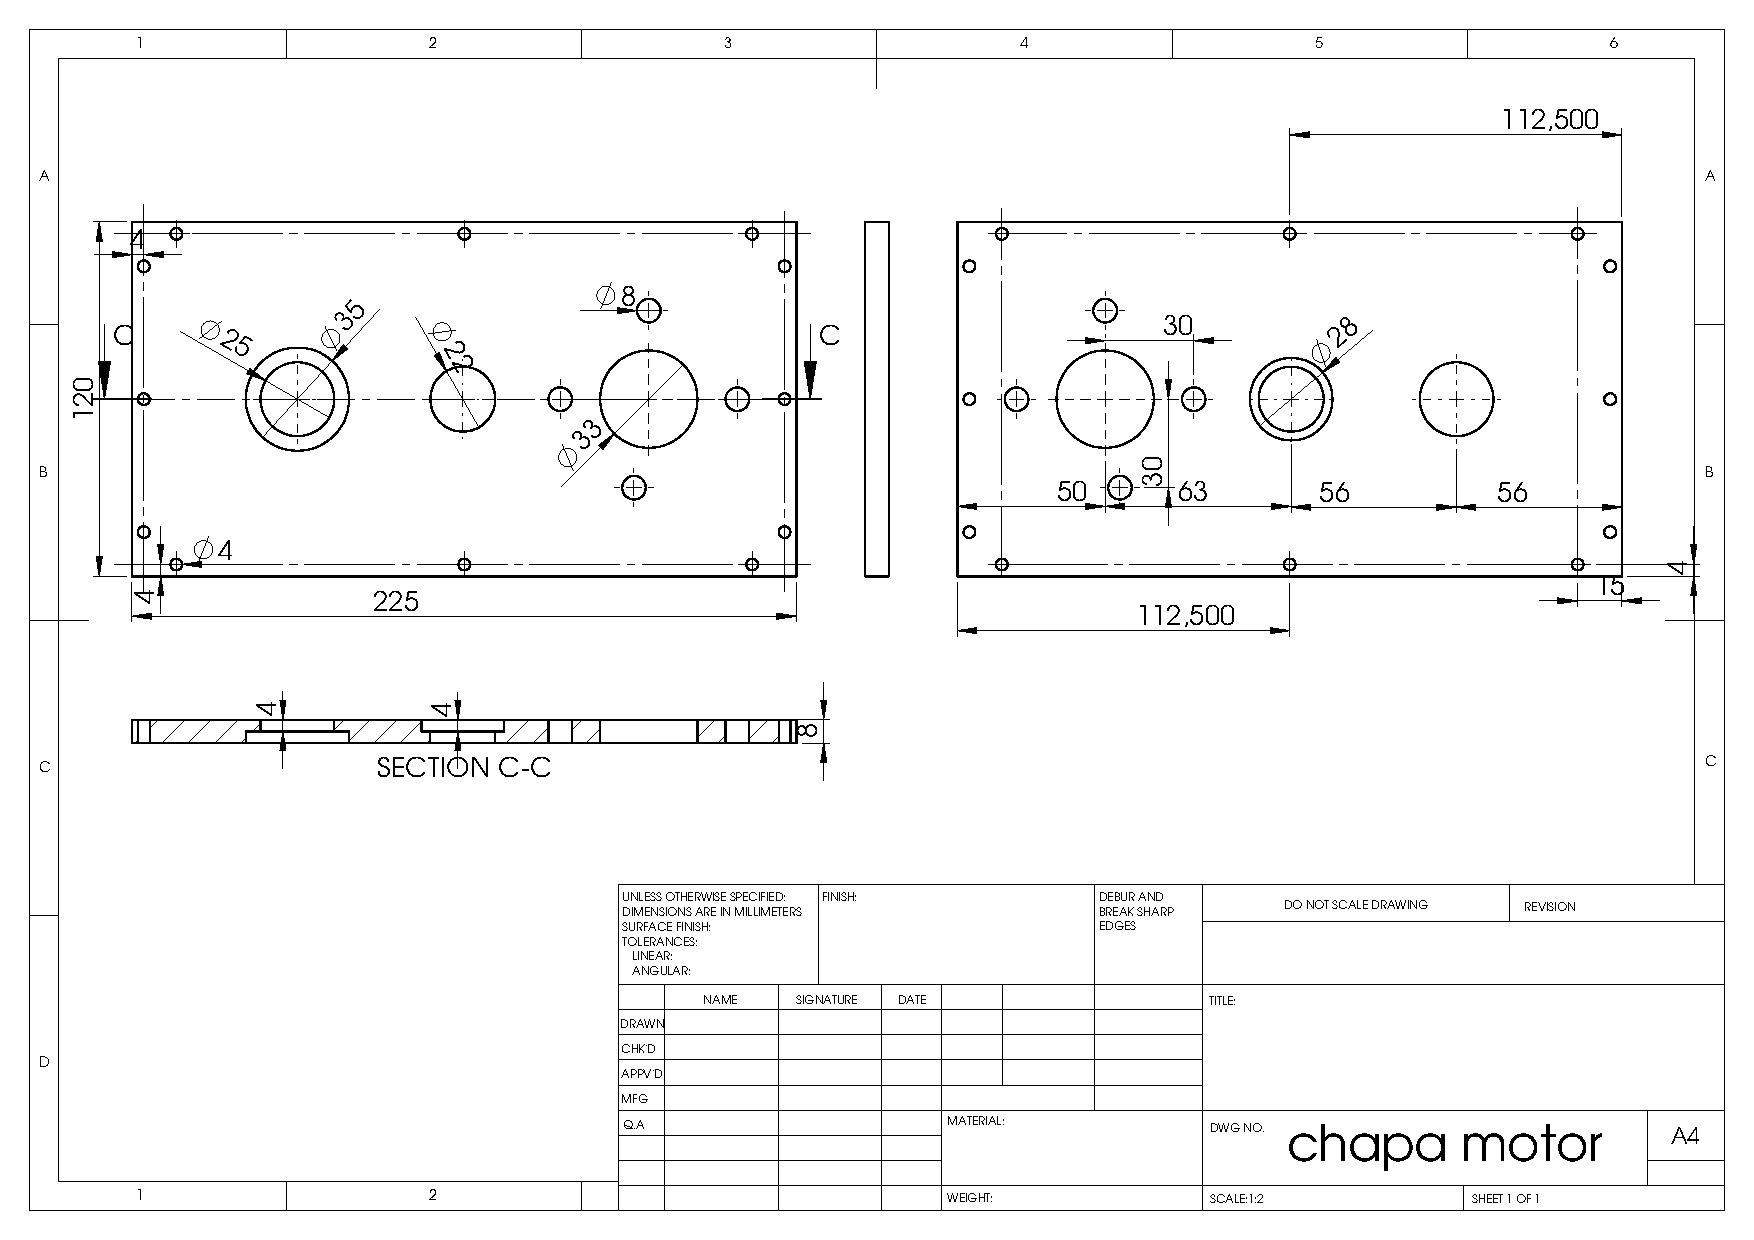
\includepdf[landscape=true]{recursos/esquemas/redutor_tracao_v1.0/chapa_lado_motor.pdf}
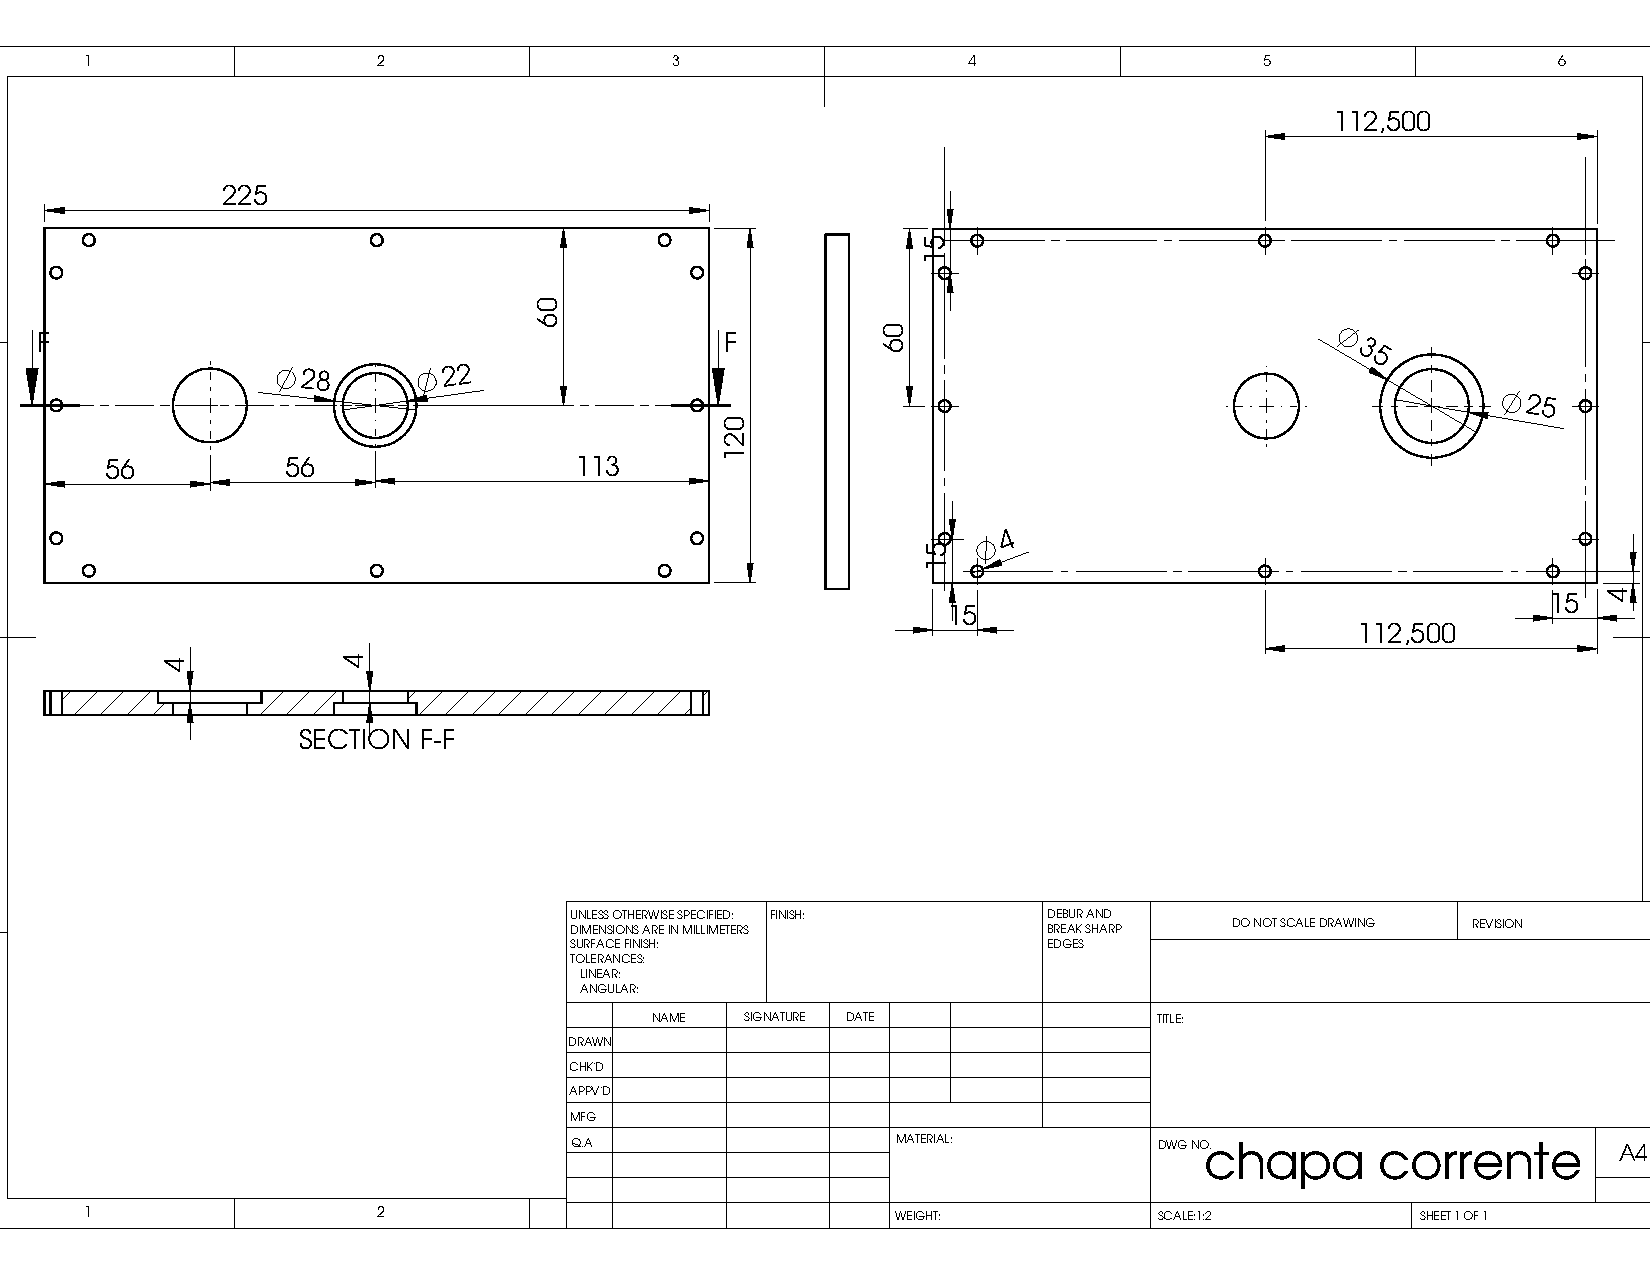
\includepdf[landscape=true]{recursos/esquemas/redutor_tracao_v1.0/chapa_lado_corrente.pdf}
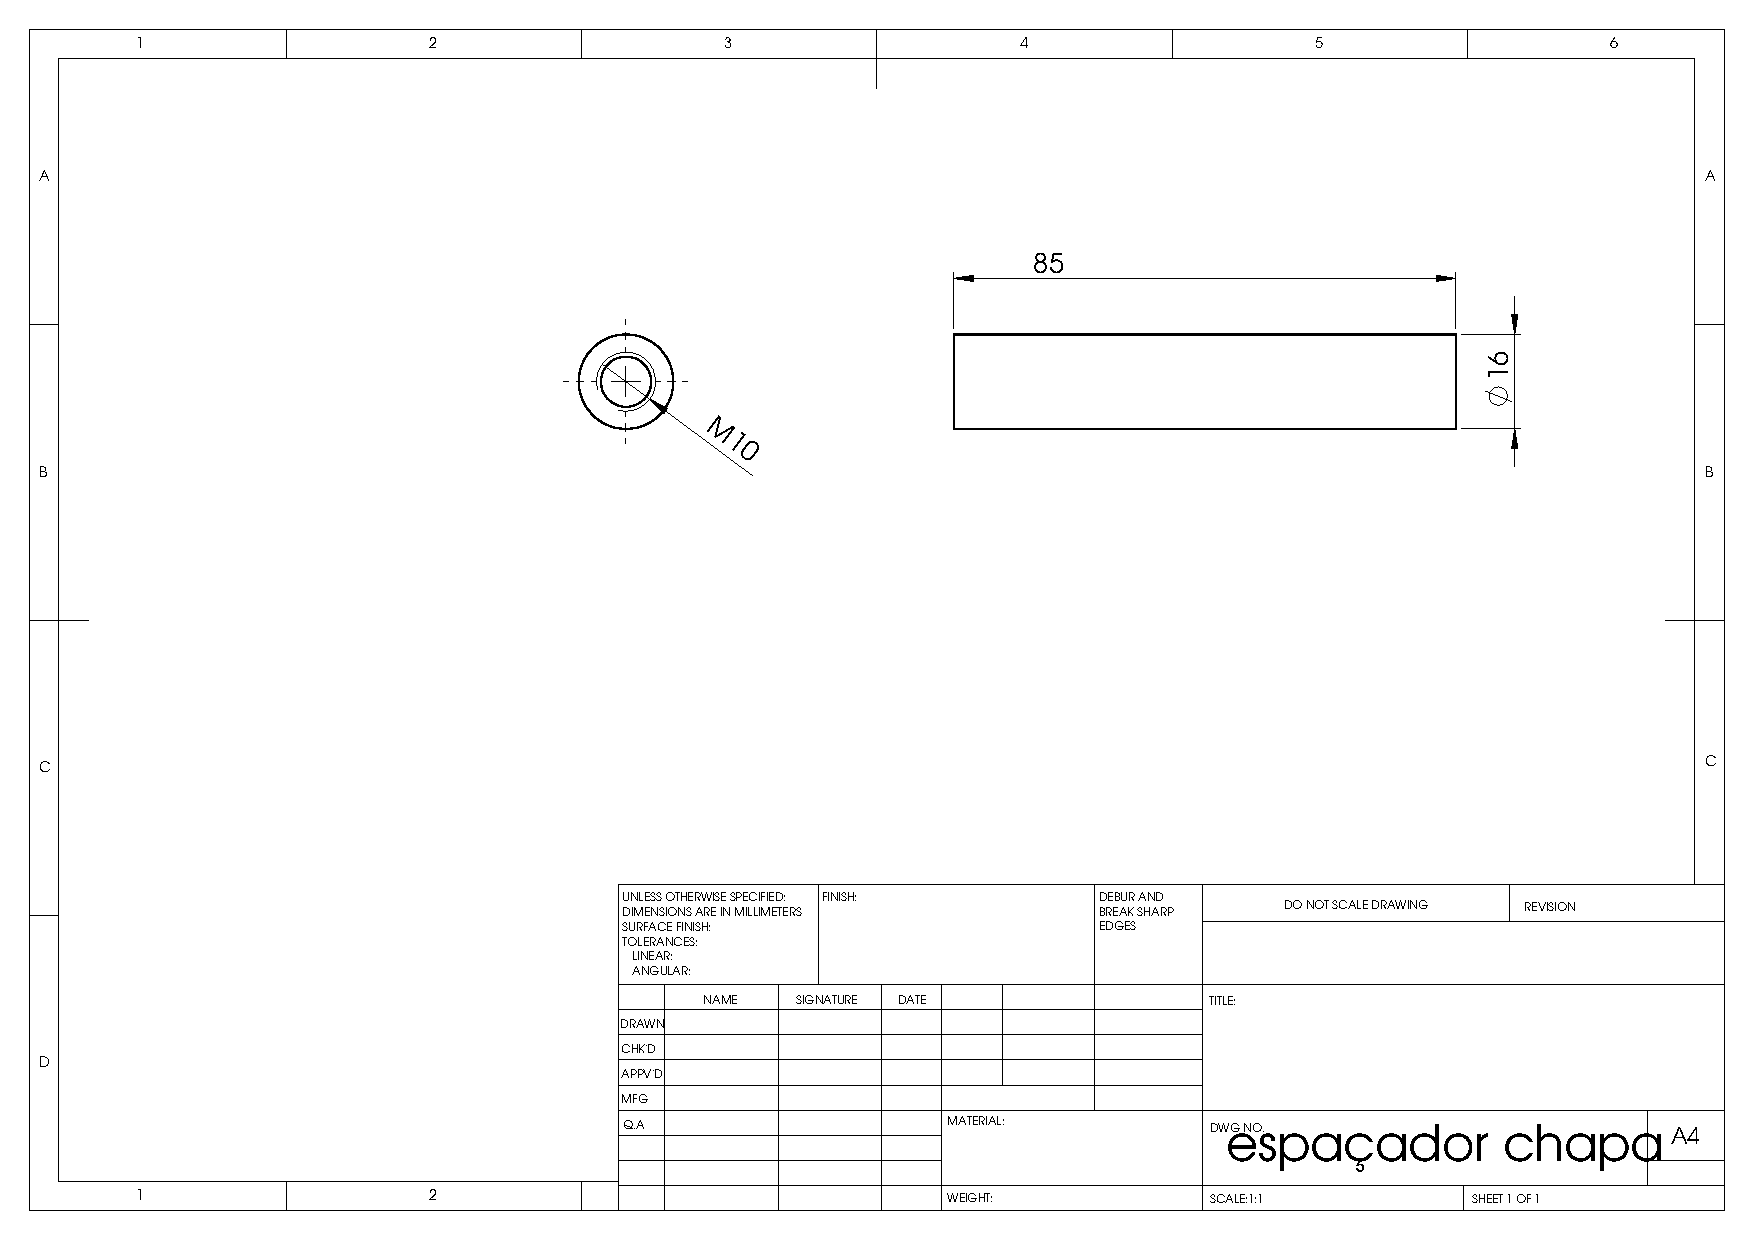
\includepdf[landscape=true]{recursos/esquemas/redutor_tracao_v1.0/espacador.pdf}
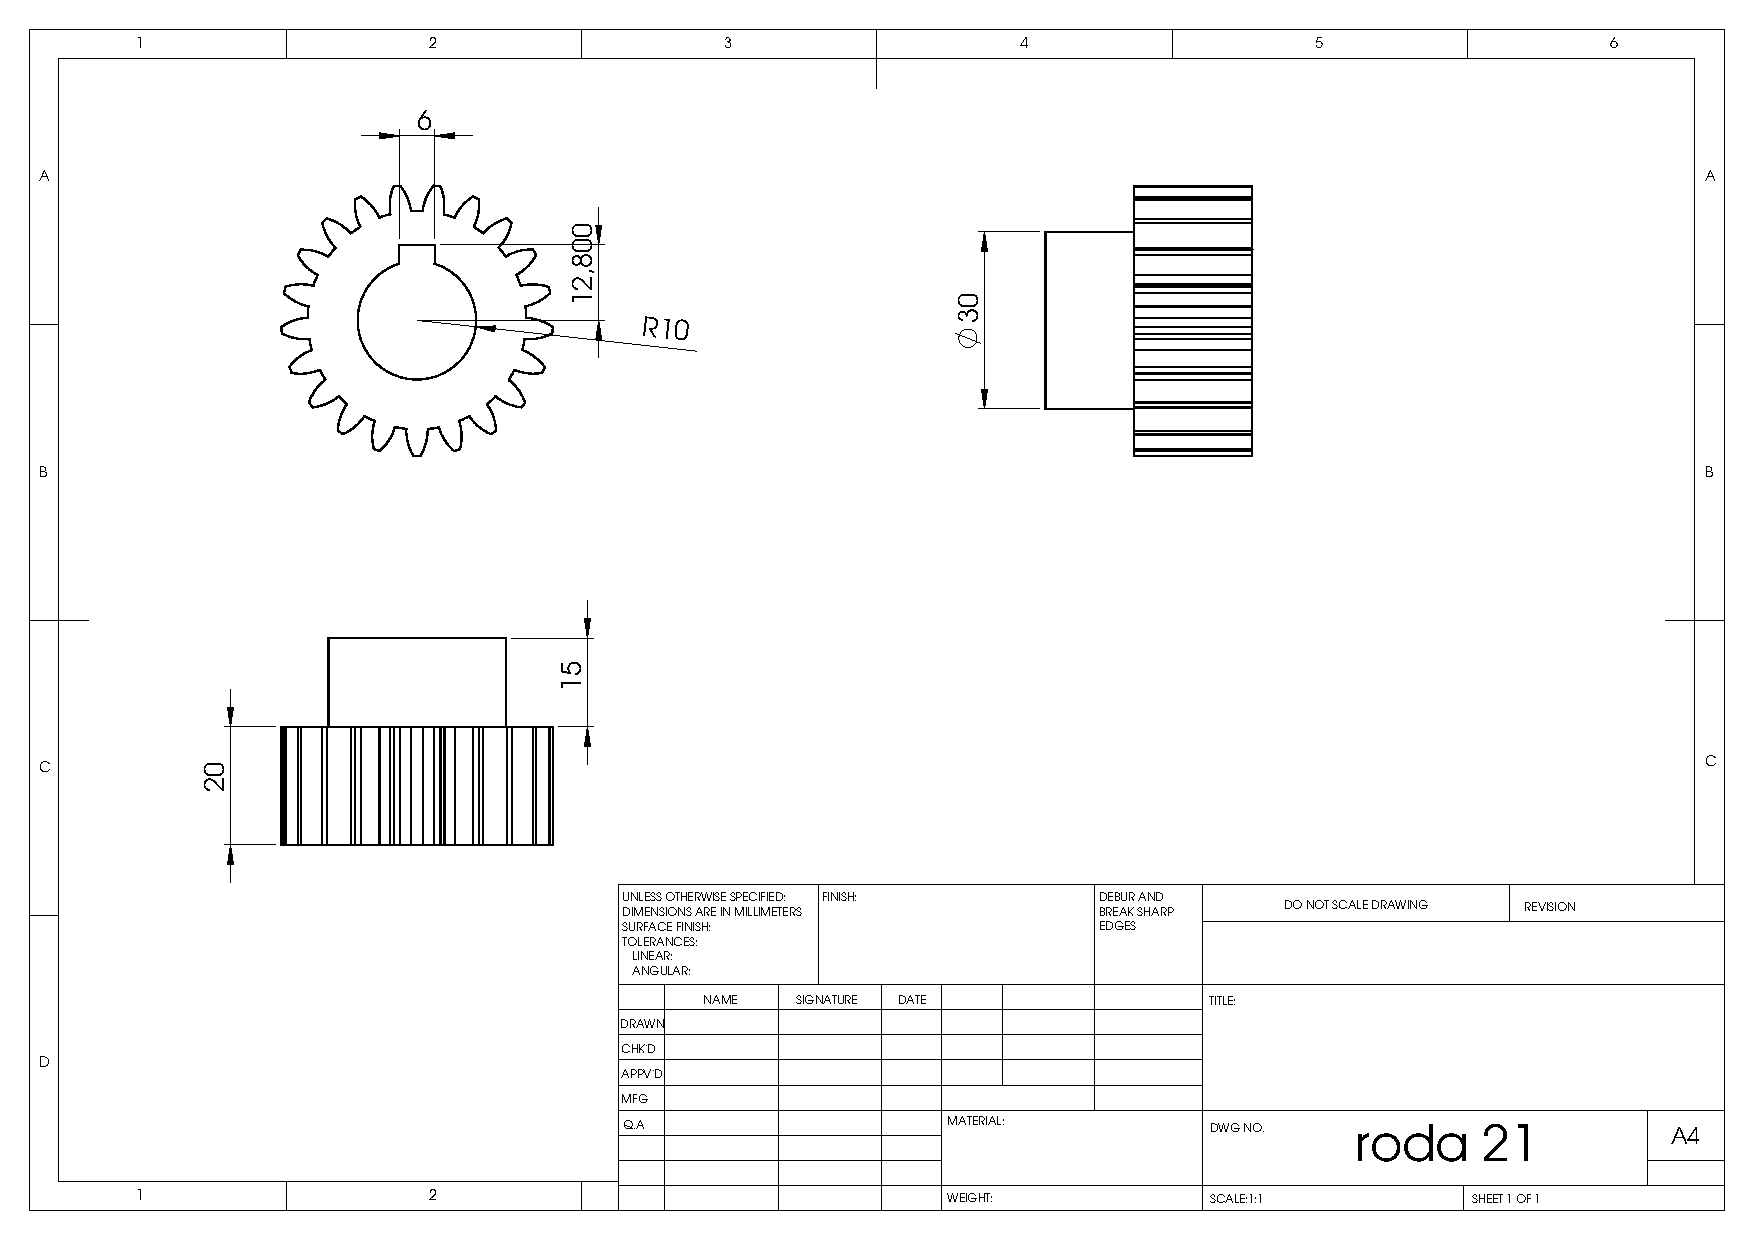
\includepdf[landscape=true]{recursos/esquemas/redutor_tracao_v1.0/engrenagem_z21.pdf}
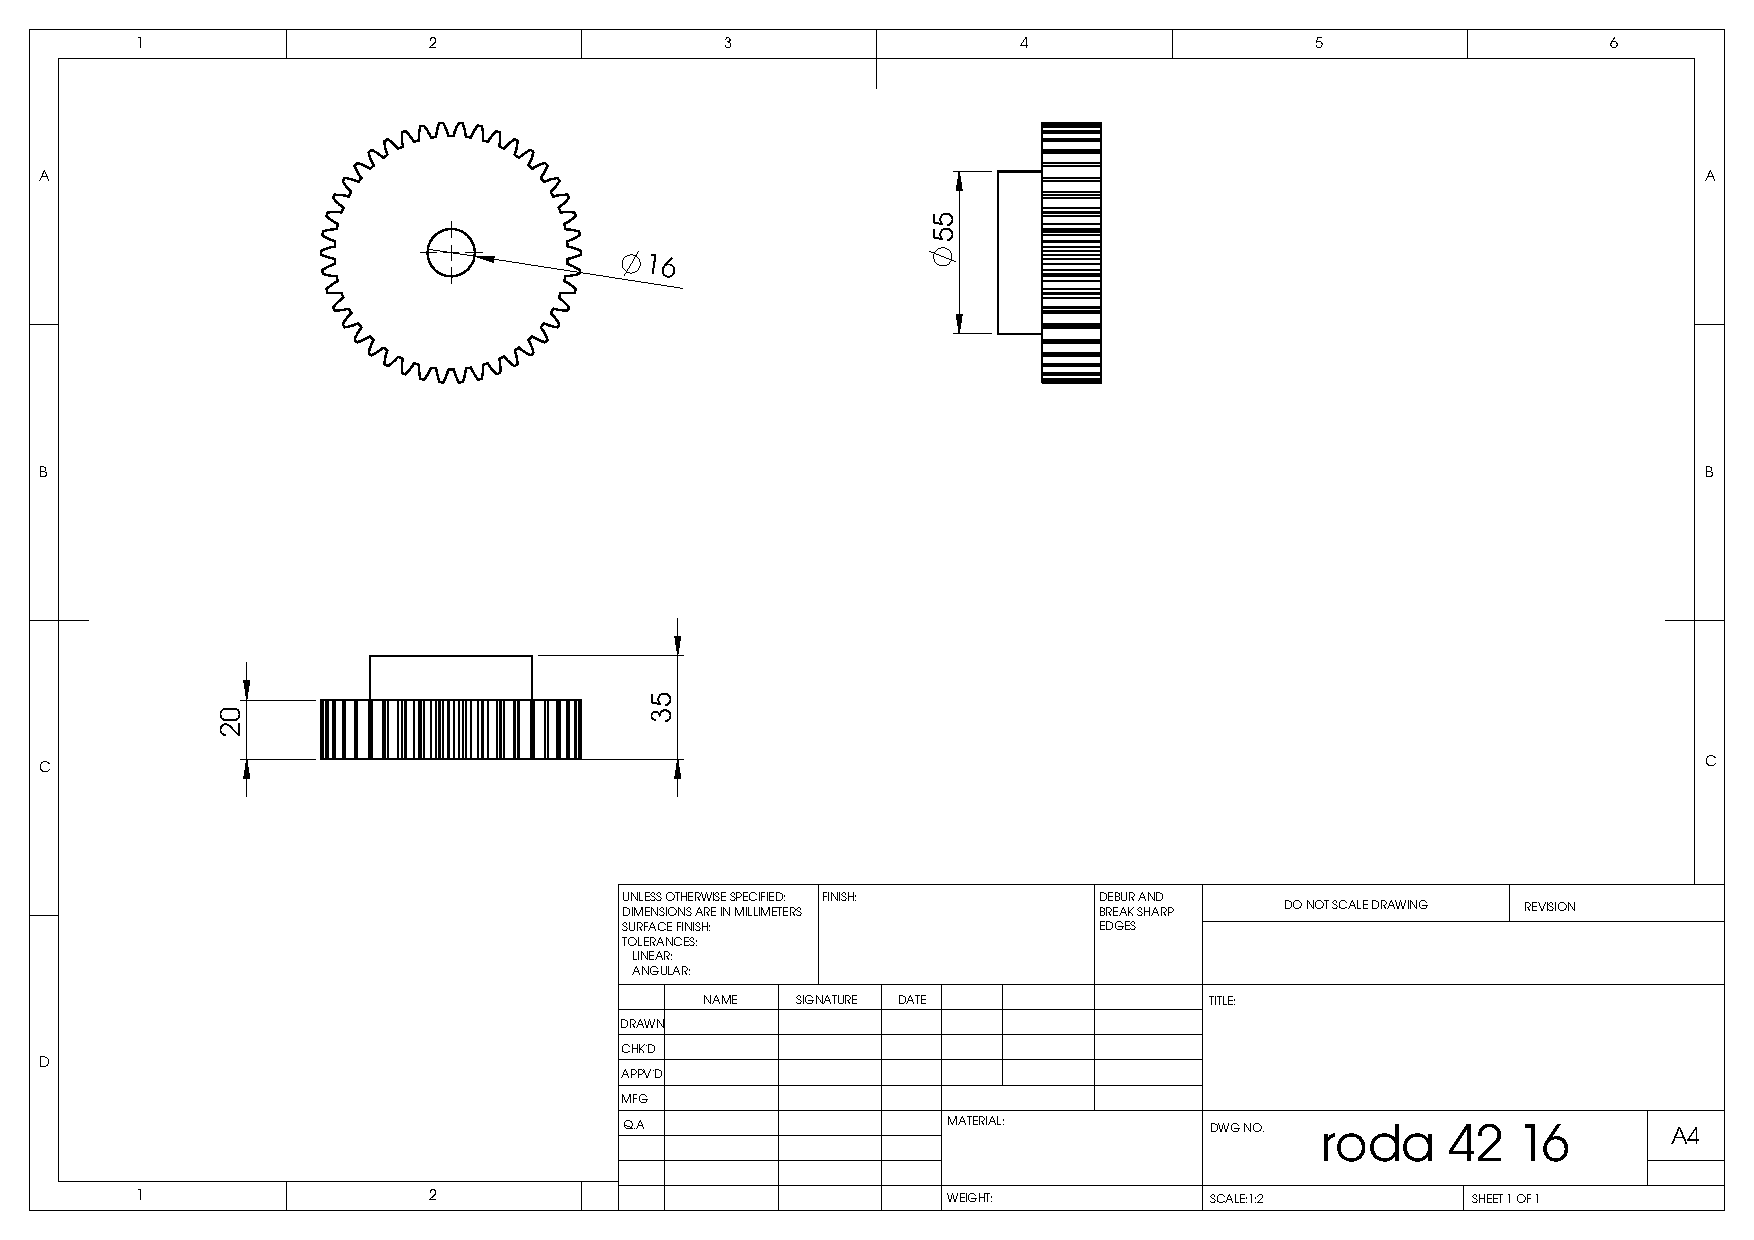
\includepdf[landscape=true]{recursos/esquemas/redutor_tracao_v1.0/engrenagem_z42_d16mm.pdf}
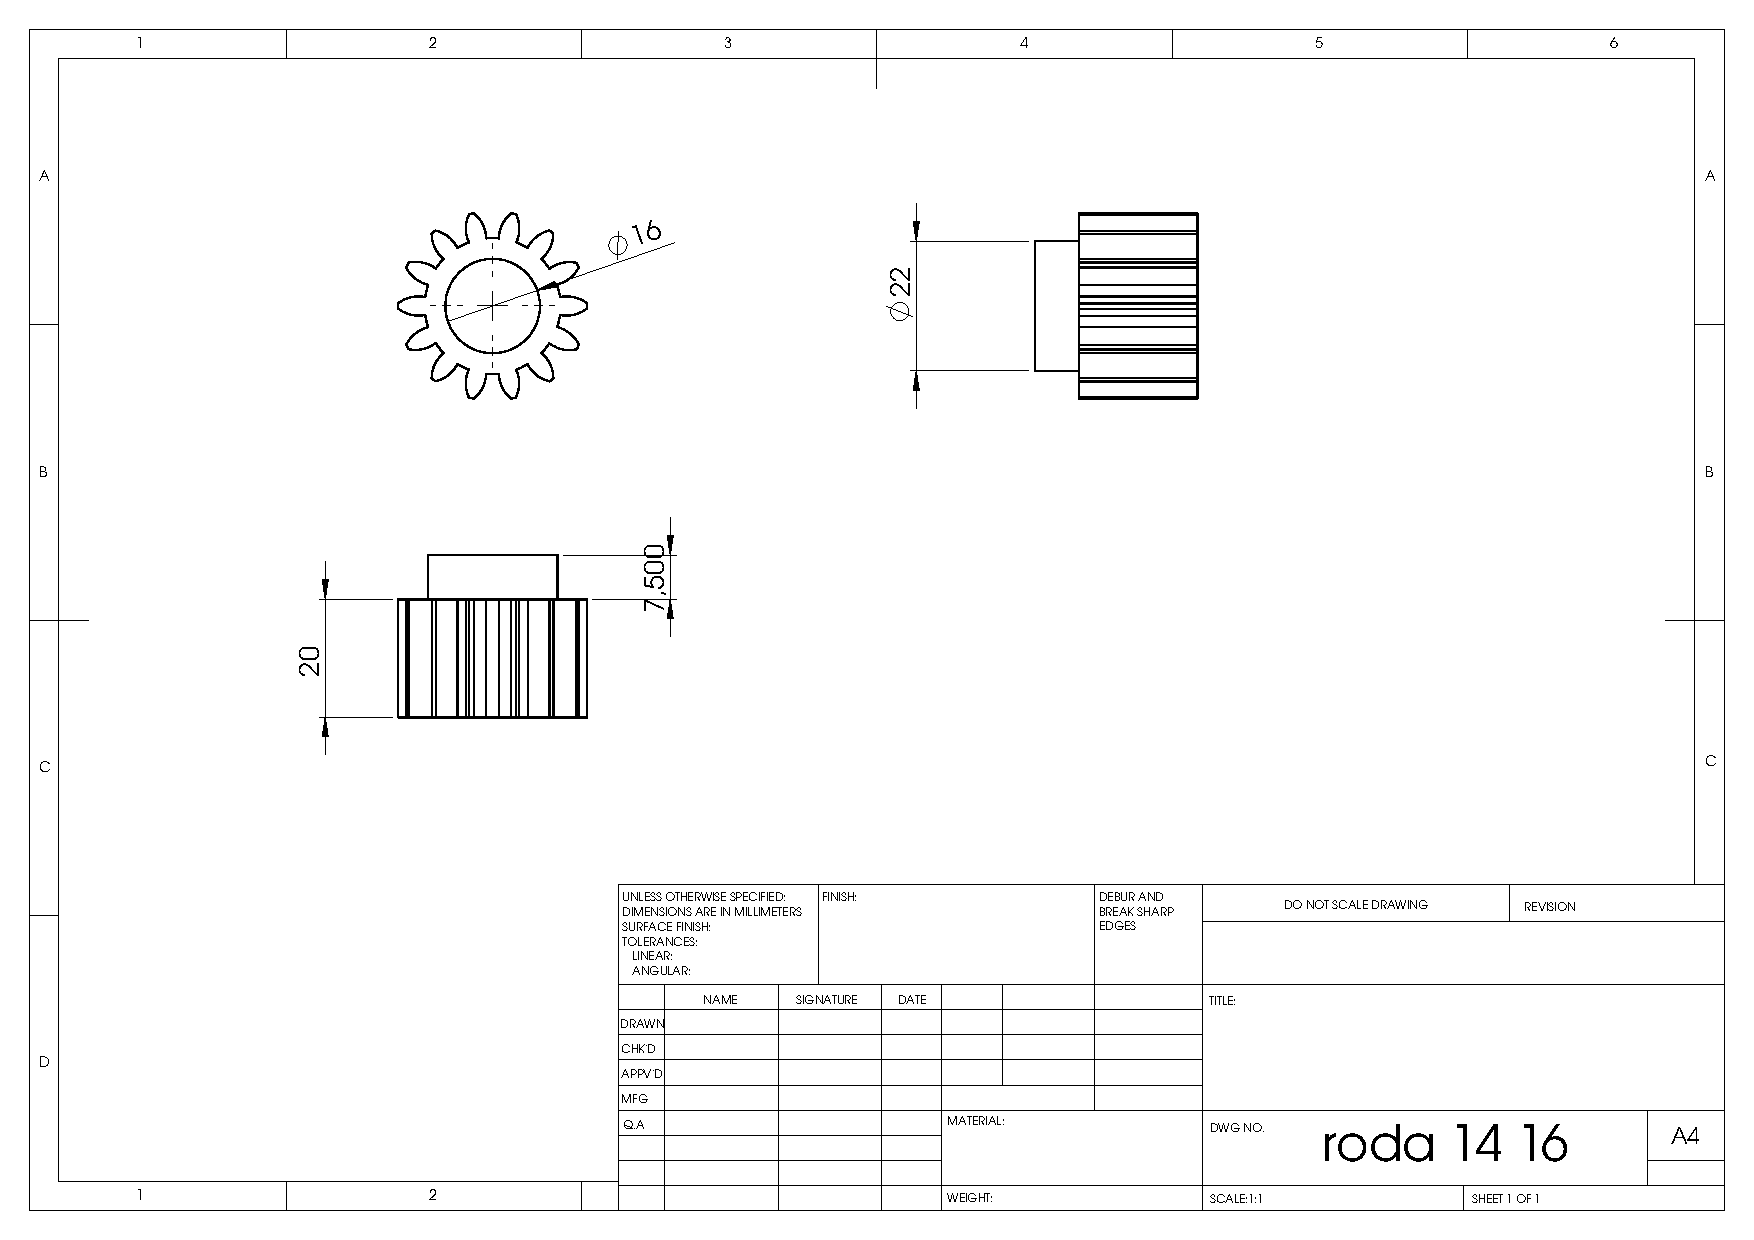
\includepdf[landscape=true]{recursos/esquemas/redutor_tracao_v1.0/engrenagem_z14.pdf}
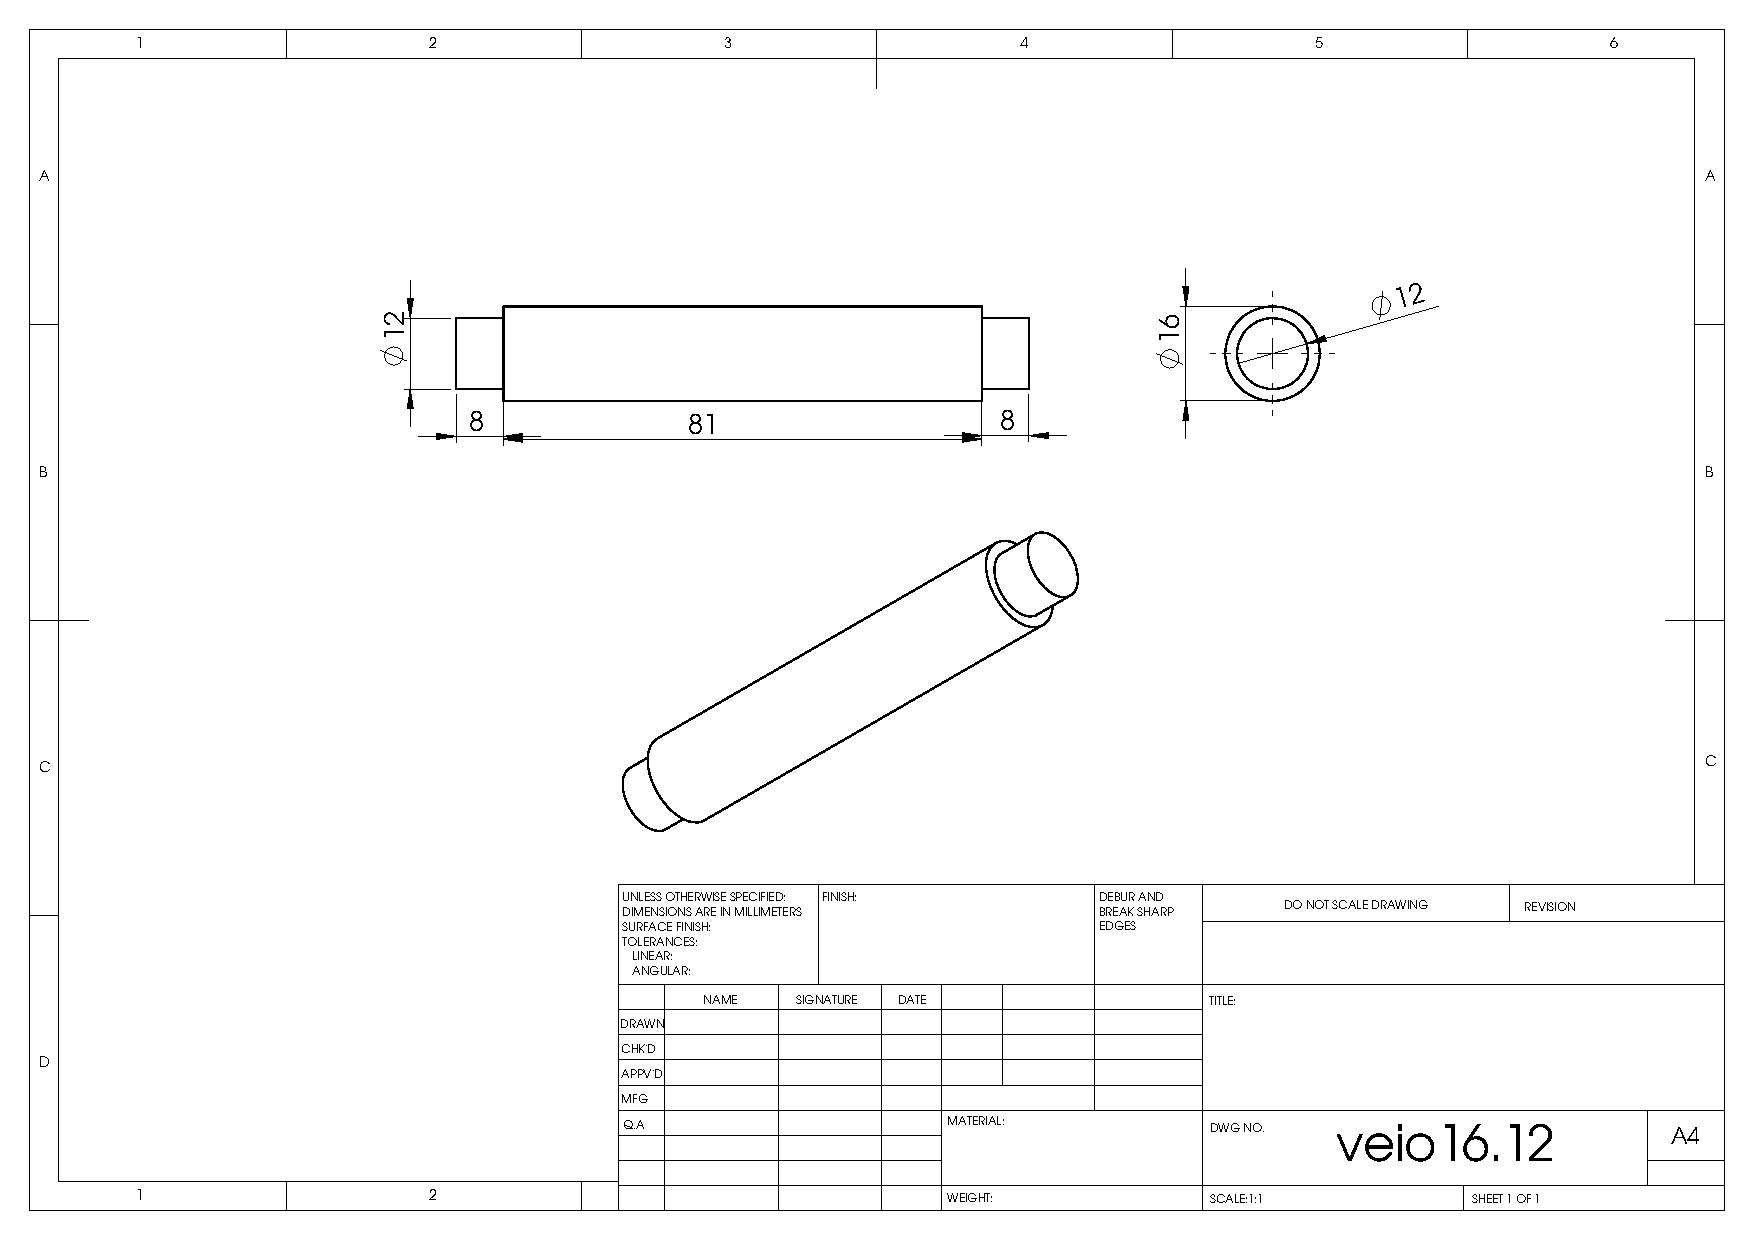
\includepdf[landscape=true]{recursos/esquemas/redutor_tracao_v1.0/veio_16_12mm.pdf}
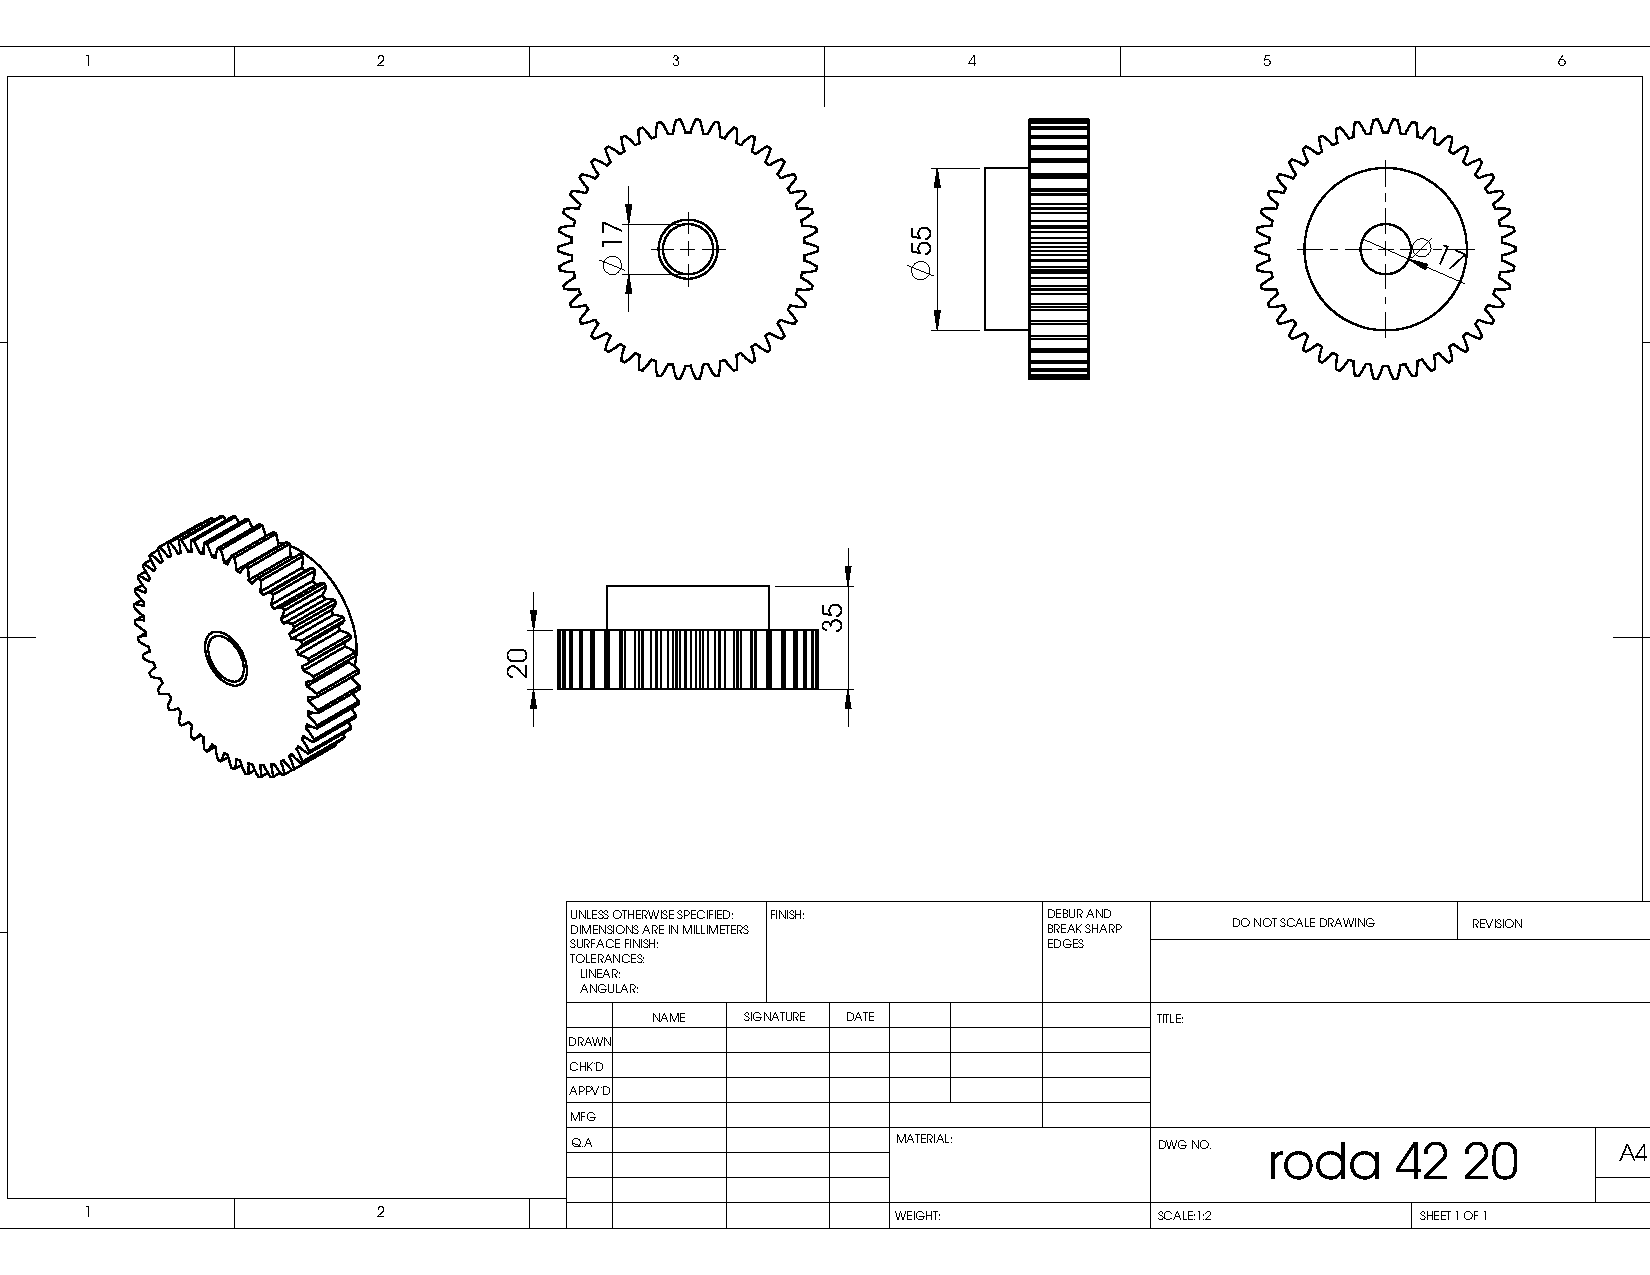
\includepdf[landscape=true]{recursos/esquemas/redutor_tracao_v1.0/engrenagem_z42_d17mm.pdf}
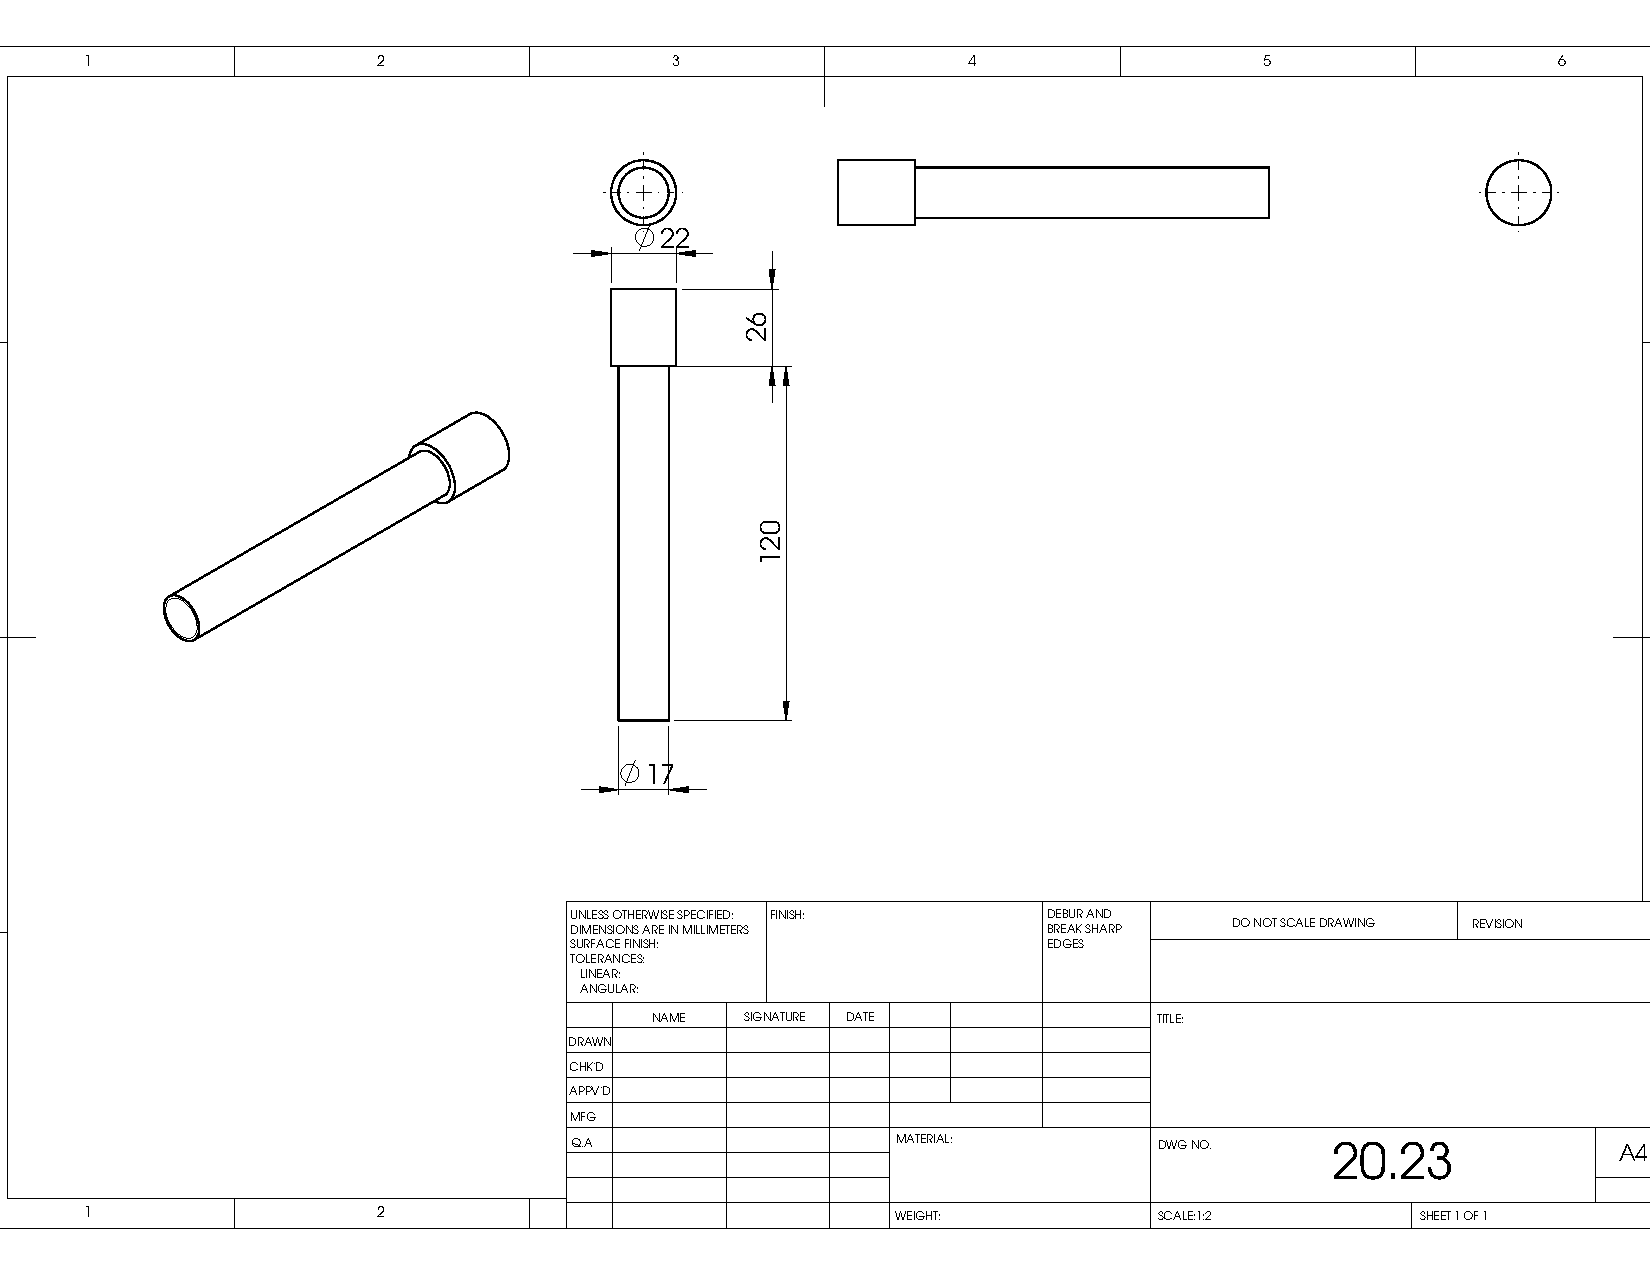
\includepdf[landscape=true]{recursos/esquemas/redutor_tracao_v1.0/veio_17_22mm.pdf}
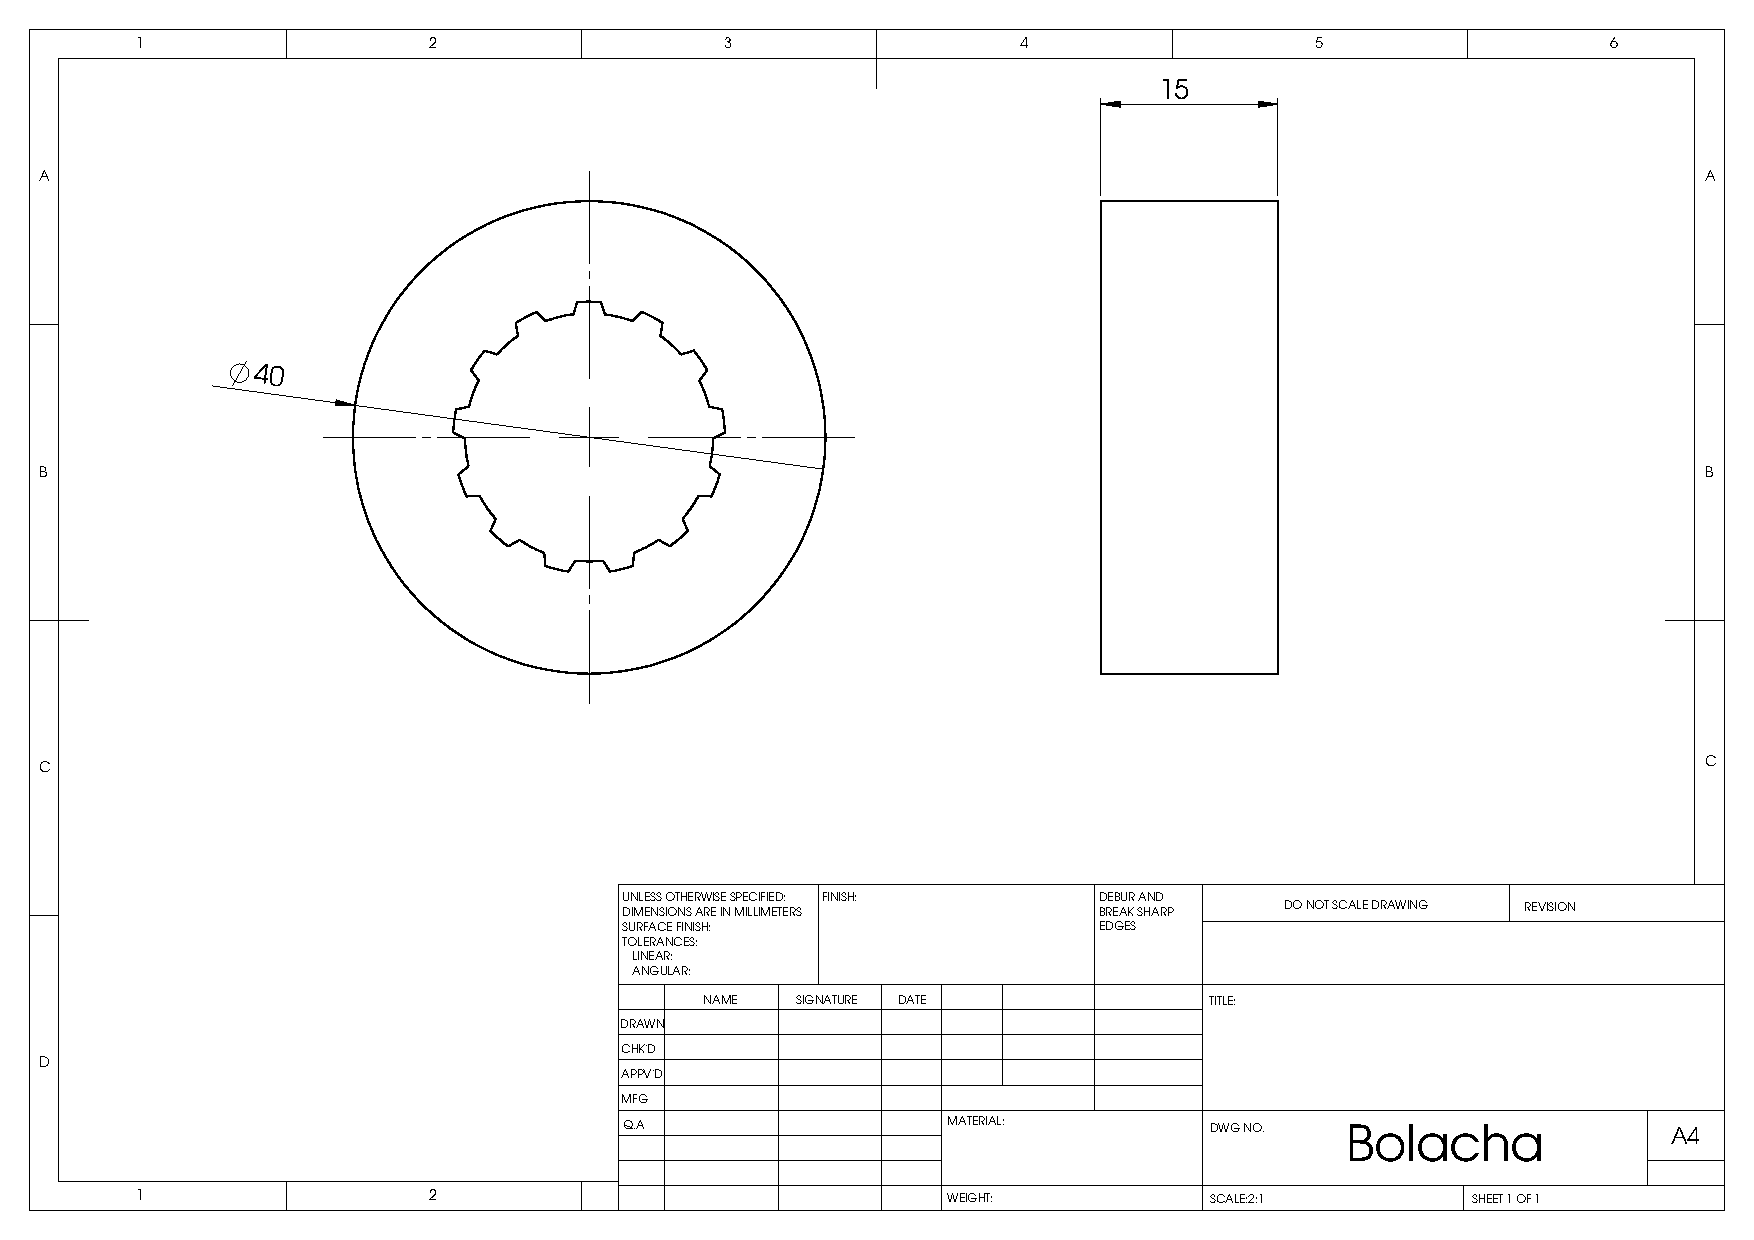
\includepdf[landscape=true]{recursos/esquemas/redutor_tracao_v1.0/bolacha_aperto_carreto.pdf}
Os desenhos deste anexo s�o uma especifica��o aproximada do redutor \emph{� priori}, com as limita��es inerentes � falta de experi�ncia do projetista. N�o contemplam alguns pormenores t�cnicos avan�ados, como toler�ncias nos encaixes, materiais a usar, e mecanismos de fixa��o. N�o substituem o parecer de t�cnicos especializados.\\
Como tal, o fabricante fez algumas modifica��es, discutidas na errata
\section*{Informa��es sobre o fabricante}
\raggedright\textbf{Vitor Ferreira \& Filhos, Lda}\\
Rua Particular � Rua Arco do Carvalh�o, Letras J.F.C, 1070 Lisboa\\
Telefone: 213884764\\
\url{www.mestredosmotores.com}
\section*{Errata}
Errata referente aos desenhos das pe�as do redutor do motor de tra��o

\todo[talking point]{Pq n�o alterei os desenhos em vez de fazer uma errata? Pq alguns par�metros foram mudados pelo torneiro durante a manufatura (ap�s o desenho da caixa), e document�-los implicaria desmontar parcialmente ou na totalidade a caixa...}
\todo{fazer as corre��es na errata e alterar o nome dos desenhos}
% If you want to place your tables where they lie in your source code and you do not need any label, do not use table at all!
\begin{center}
    %Tried using tabularx and tabulary, and both sucked - could not handle the extra large column well.
    \begin{tabular}{b{0.15\textwidth} b{0.15\textwidth} b{0.6\textwidth}}
        \textbf{Desenho} & \textbf{Onde se l�/v�} & \textbf{Deve l�r-se/v�r-se}\\ \midrule
        espa�ador chapa & 85 & 87\\
        roda 21 & R10 & R9.5\\
        roda 21 & 12.800 & 12.300\\
        roda 21 & & Chave (paralelip�pedo quadrangular com 6 mm de lado, cantos arredondados e 35 mm de comprimento) para prender engrenagem de 21 dentes ao veio do motor, de acordo com a norma ISO/R773 \cite{norma_ISO_R773}.\\
        20.23 & Face do veio \diameter22 liso & Face do veio \diameter22 liso at� 11mm ap�s o \diameter17. Da� at� ao topo, veio maquinado para encaixe no buraco da bolacha do desenho "bolacha".\todo[talking point]{com a largura do carreto, a bolacha n�o entra totalmente no veio.}\\
        20.23 & Topo do veio \diameter22 liso & Topo do veio \diameter22 com rosca M8 conc�ntrica.\\
        20.23 & 120 & 115, medidos a partir do veio \diameter22. Ranhura para freio ap�s a medida.\todo{confirmar}\\
        bolacha & & Um dos topos do cilindro tapado, com um furo M8 conc�ntrico.\\
        chapa corrente & 12 furos de 4 mm & 4 furos M10 pr�ximos dos cantos da placa.\\
        chapa motor & 12 furos de 4 mm & 4 furos M10 pr�ximos dos cantos da placa, � mesma dist�ncia dos da errata do desenho "chapa corrente".\\
        montagem & Veio do motor & Espa�ador cil�ndrico com furo conc�ntrico de 19 mm e cerca de 3 mm de largura, montado no veio, antes da engrenagem.\\
    \end{tabular}
\end{center}

        
\fancychapter{Ap�ndice E - desenhos t�cnicos das pe�as do redutor do motor de tra��o}
\label{ap:e}

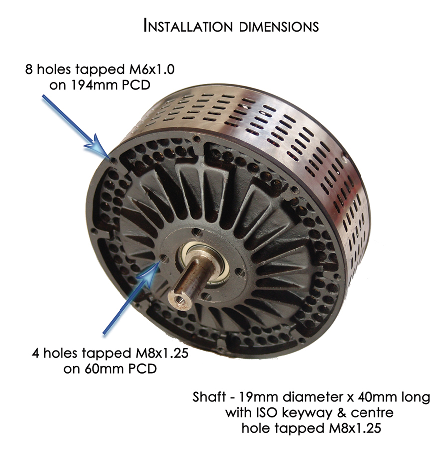
\includepdf[landscape=true]{recursos/esquemas/redutor_tracao_v1.0/motor.pdf}
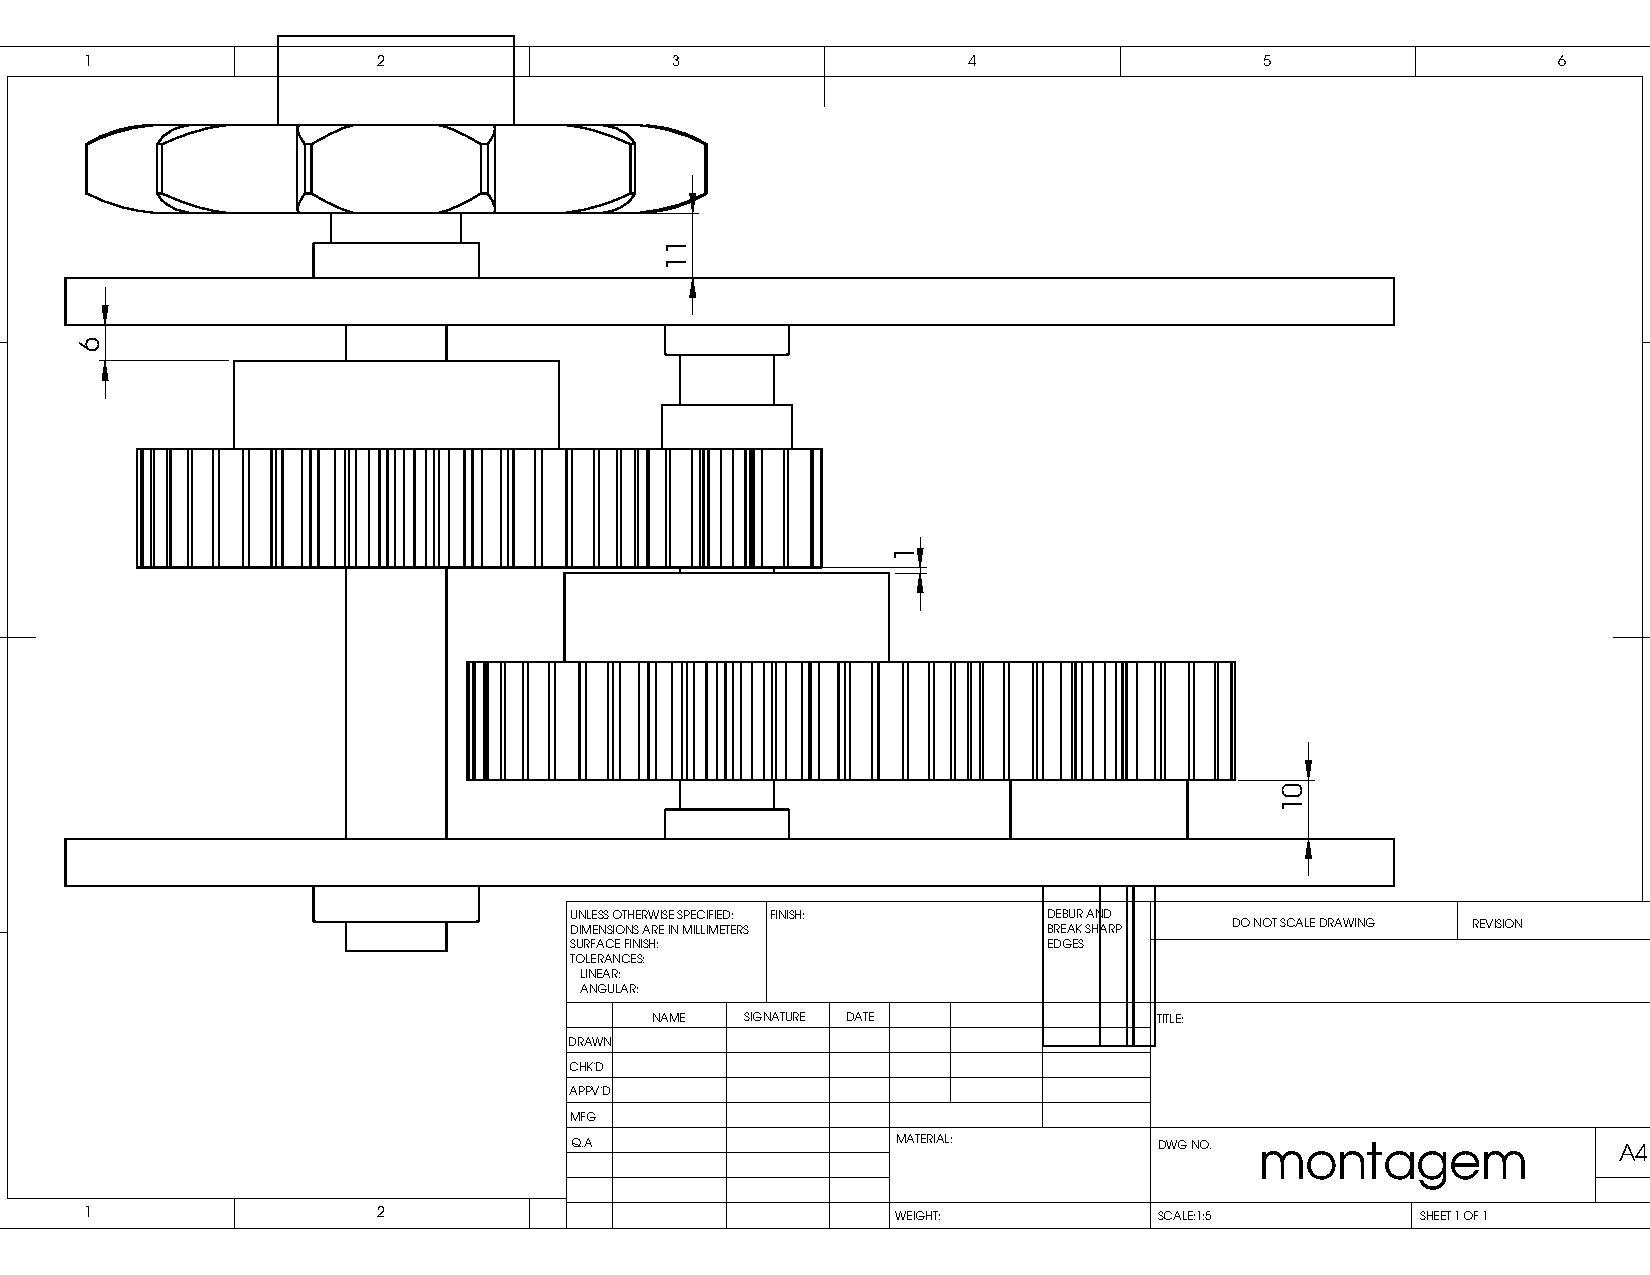
\includepdf[landscape=true]{recursos/esquemas/redutor_tracao_v1.0/montagem_vista_cima.pdf}
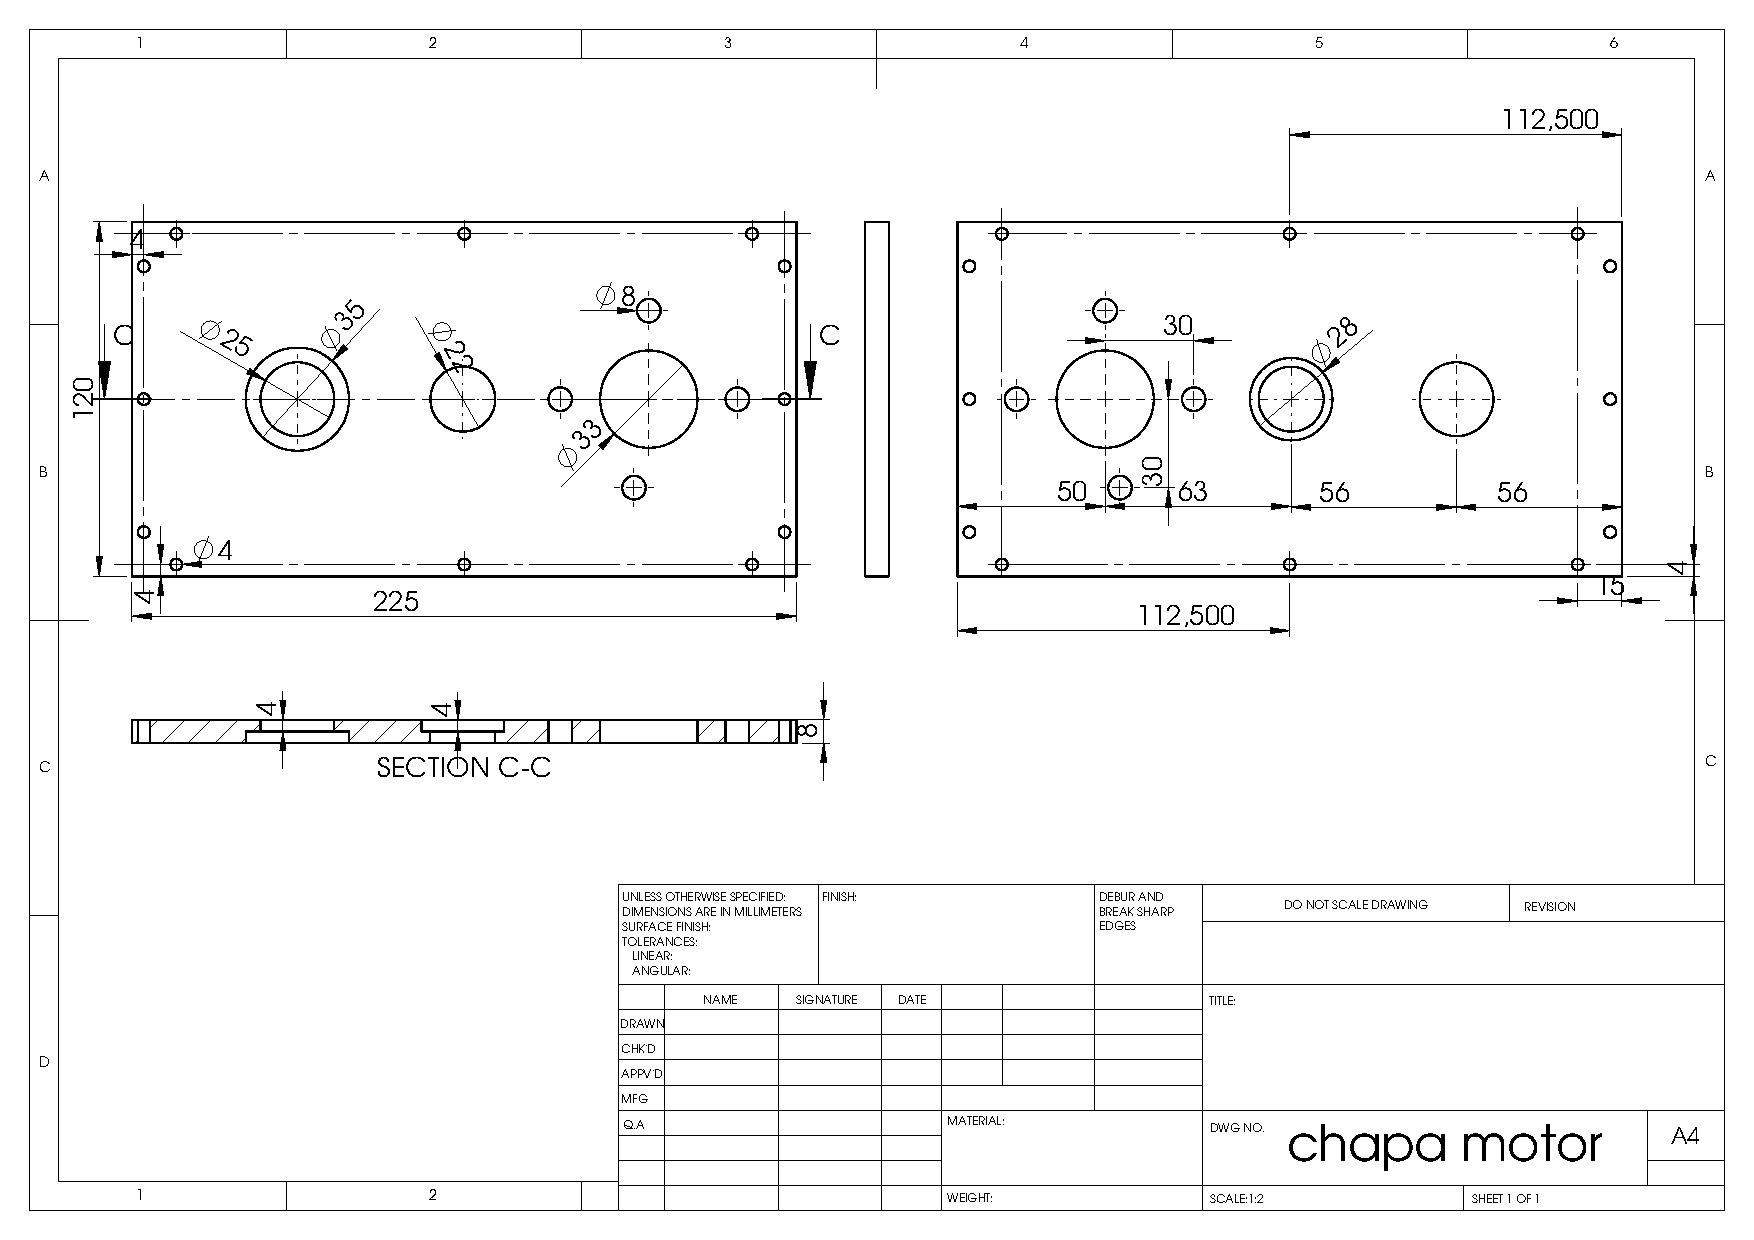
\includepdf[landscape=true]{recursos/esquemas/redutor_tracao_v1.0/chapa_lado_motor.pdf}
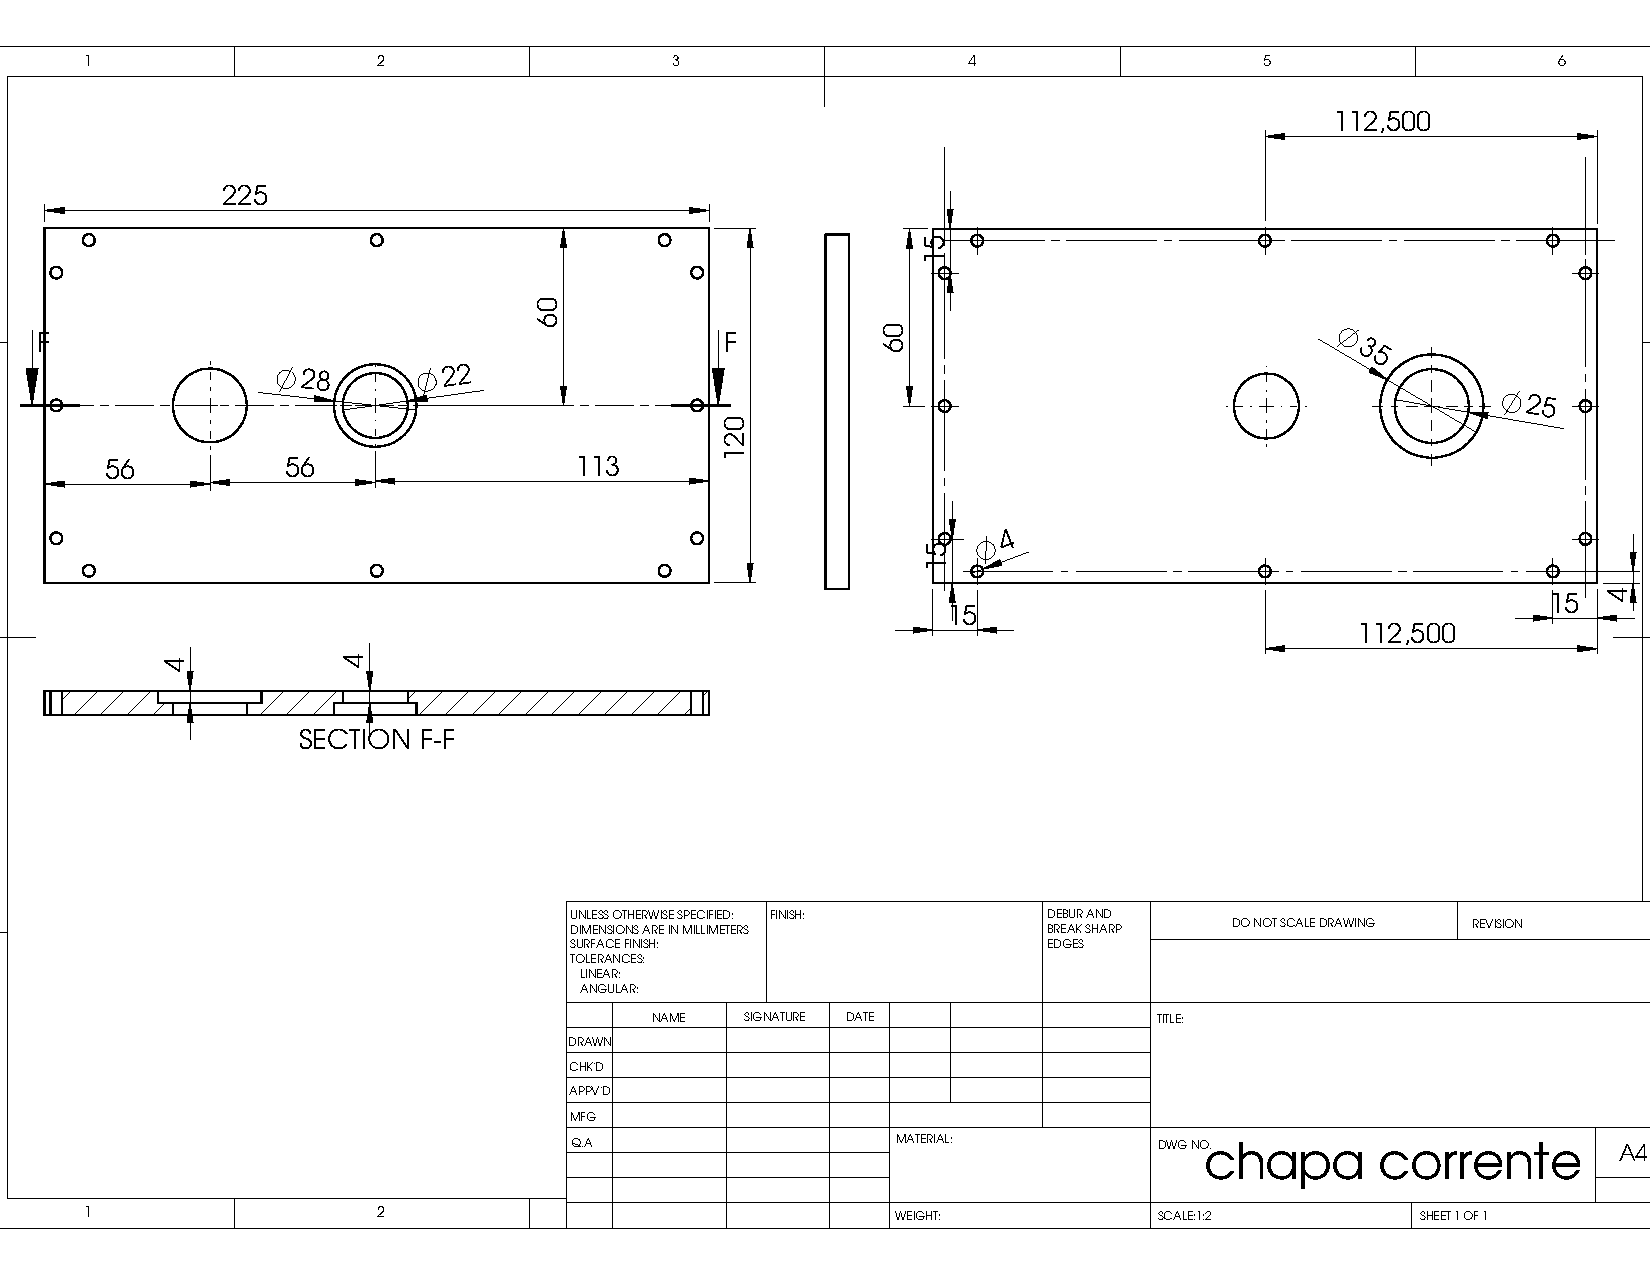
\includepdf[landscape=true]{recursos/esquemas/redutor_tracao_v1.0/chapa_lado_corrente.pdf}
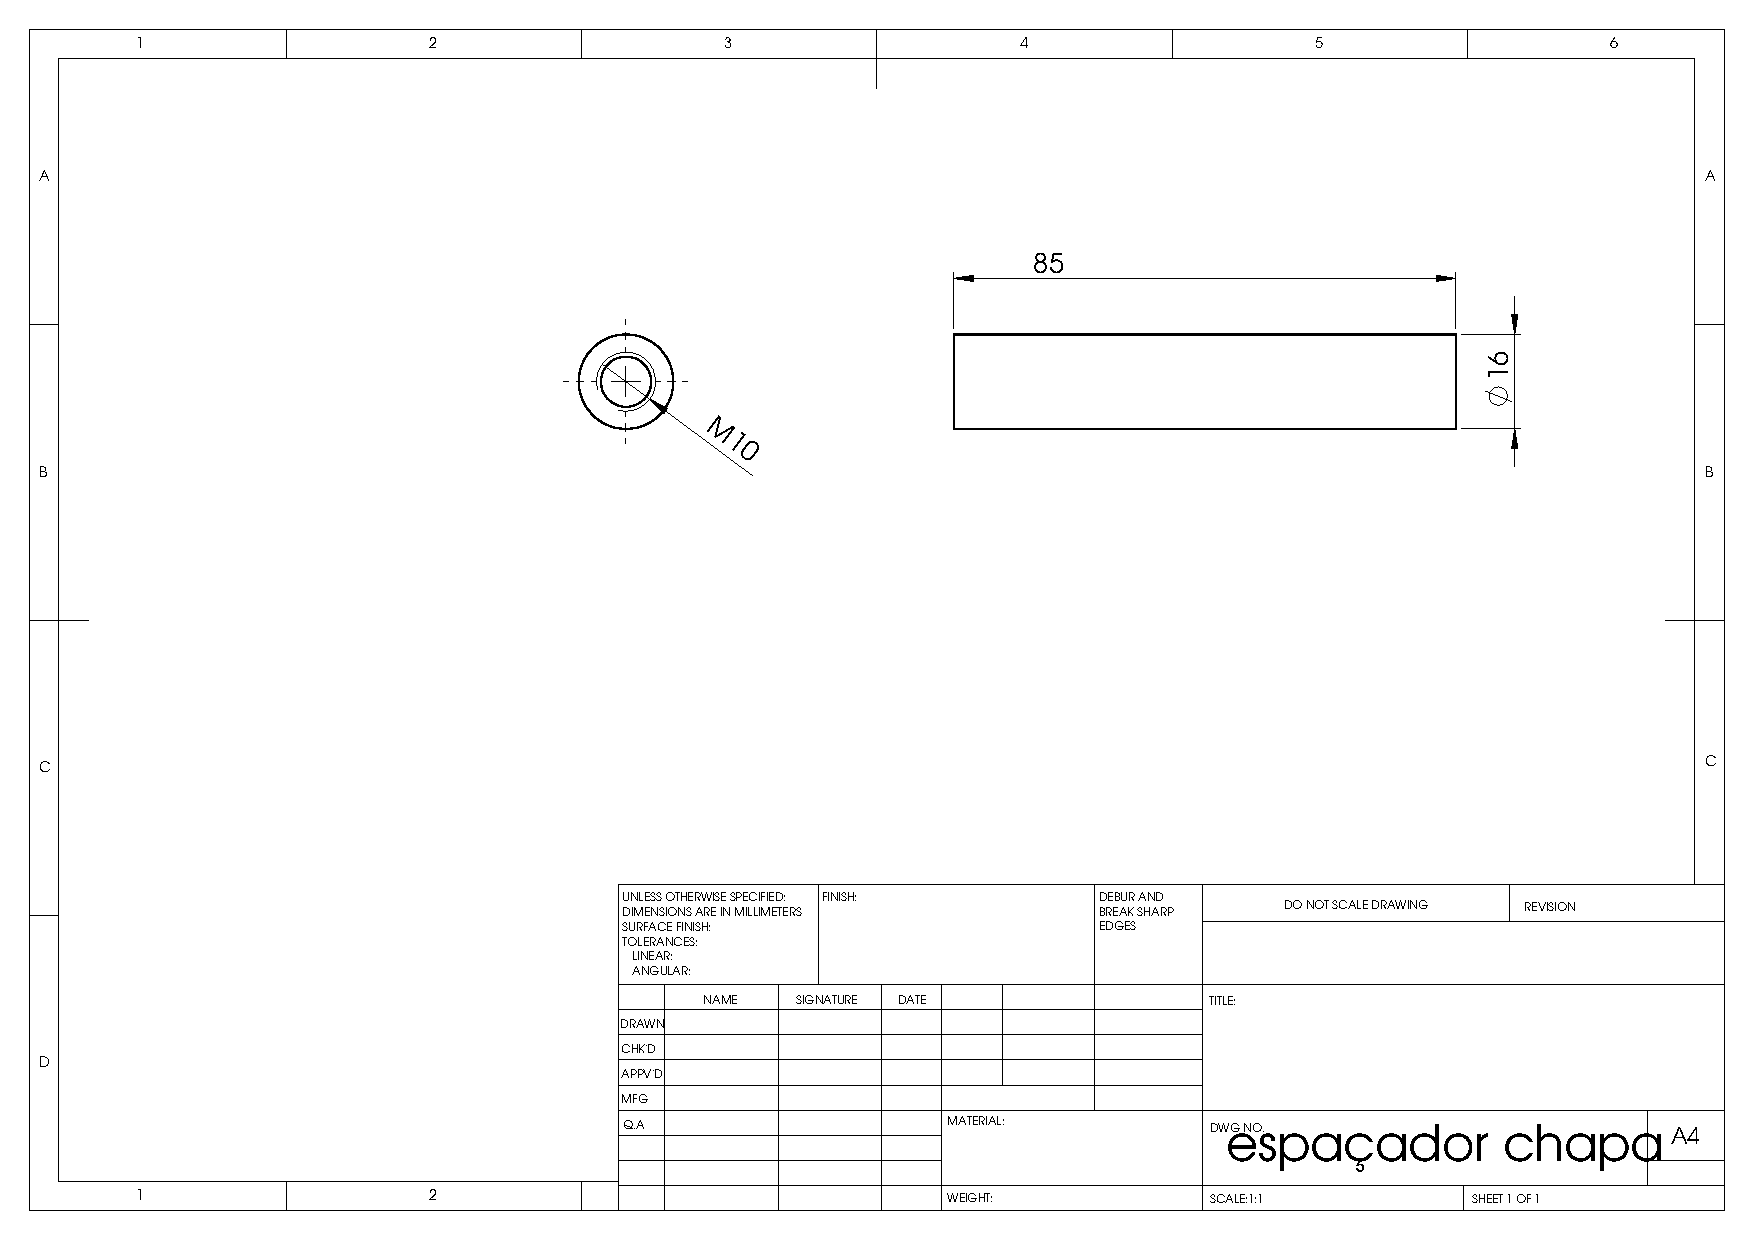
\includepdf[landscape=true]{recursos/esquemas/redutor_tracao_v1.0/espacador.pdf}
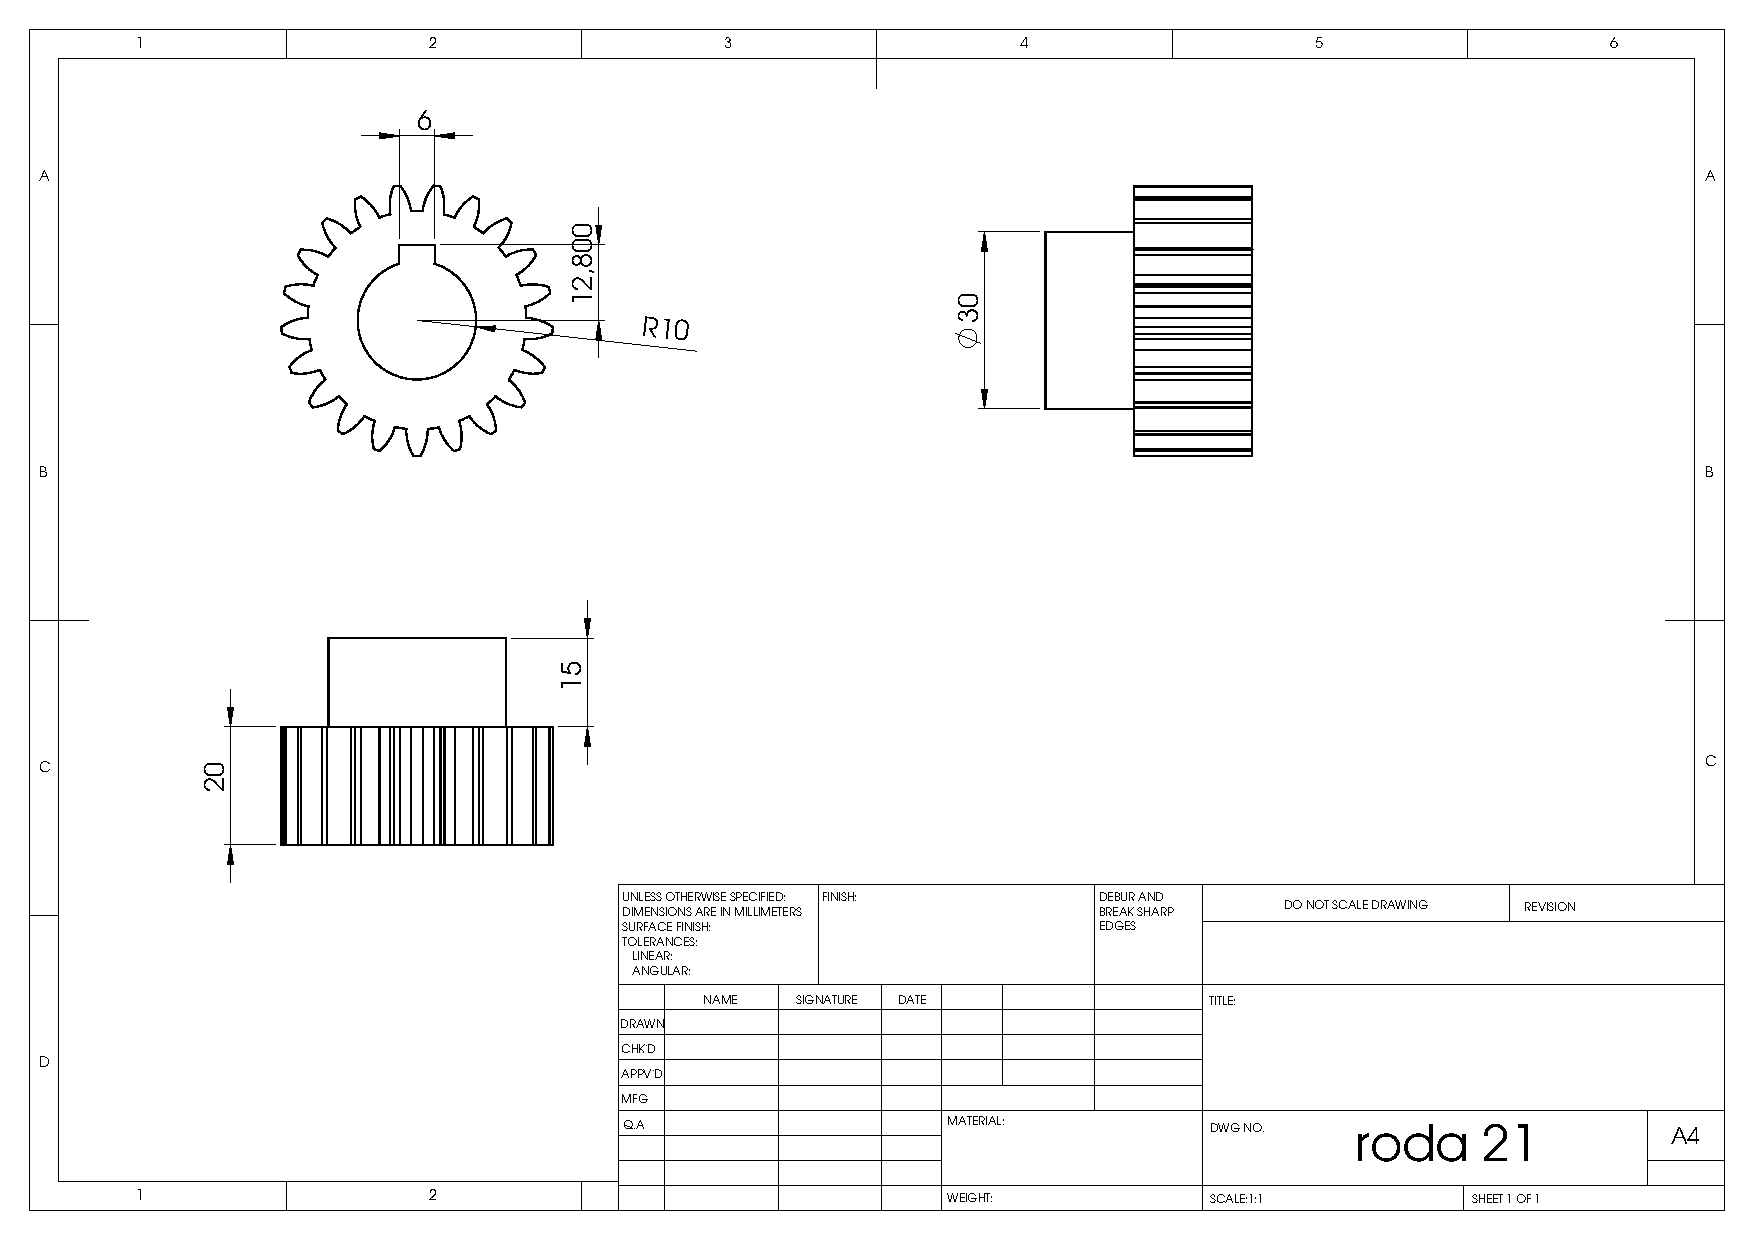
\includepdf[landscape=true]{recursos/esquemas/redutor_tracao_v1.0/engrenagem_z21.pdf}
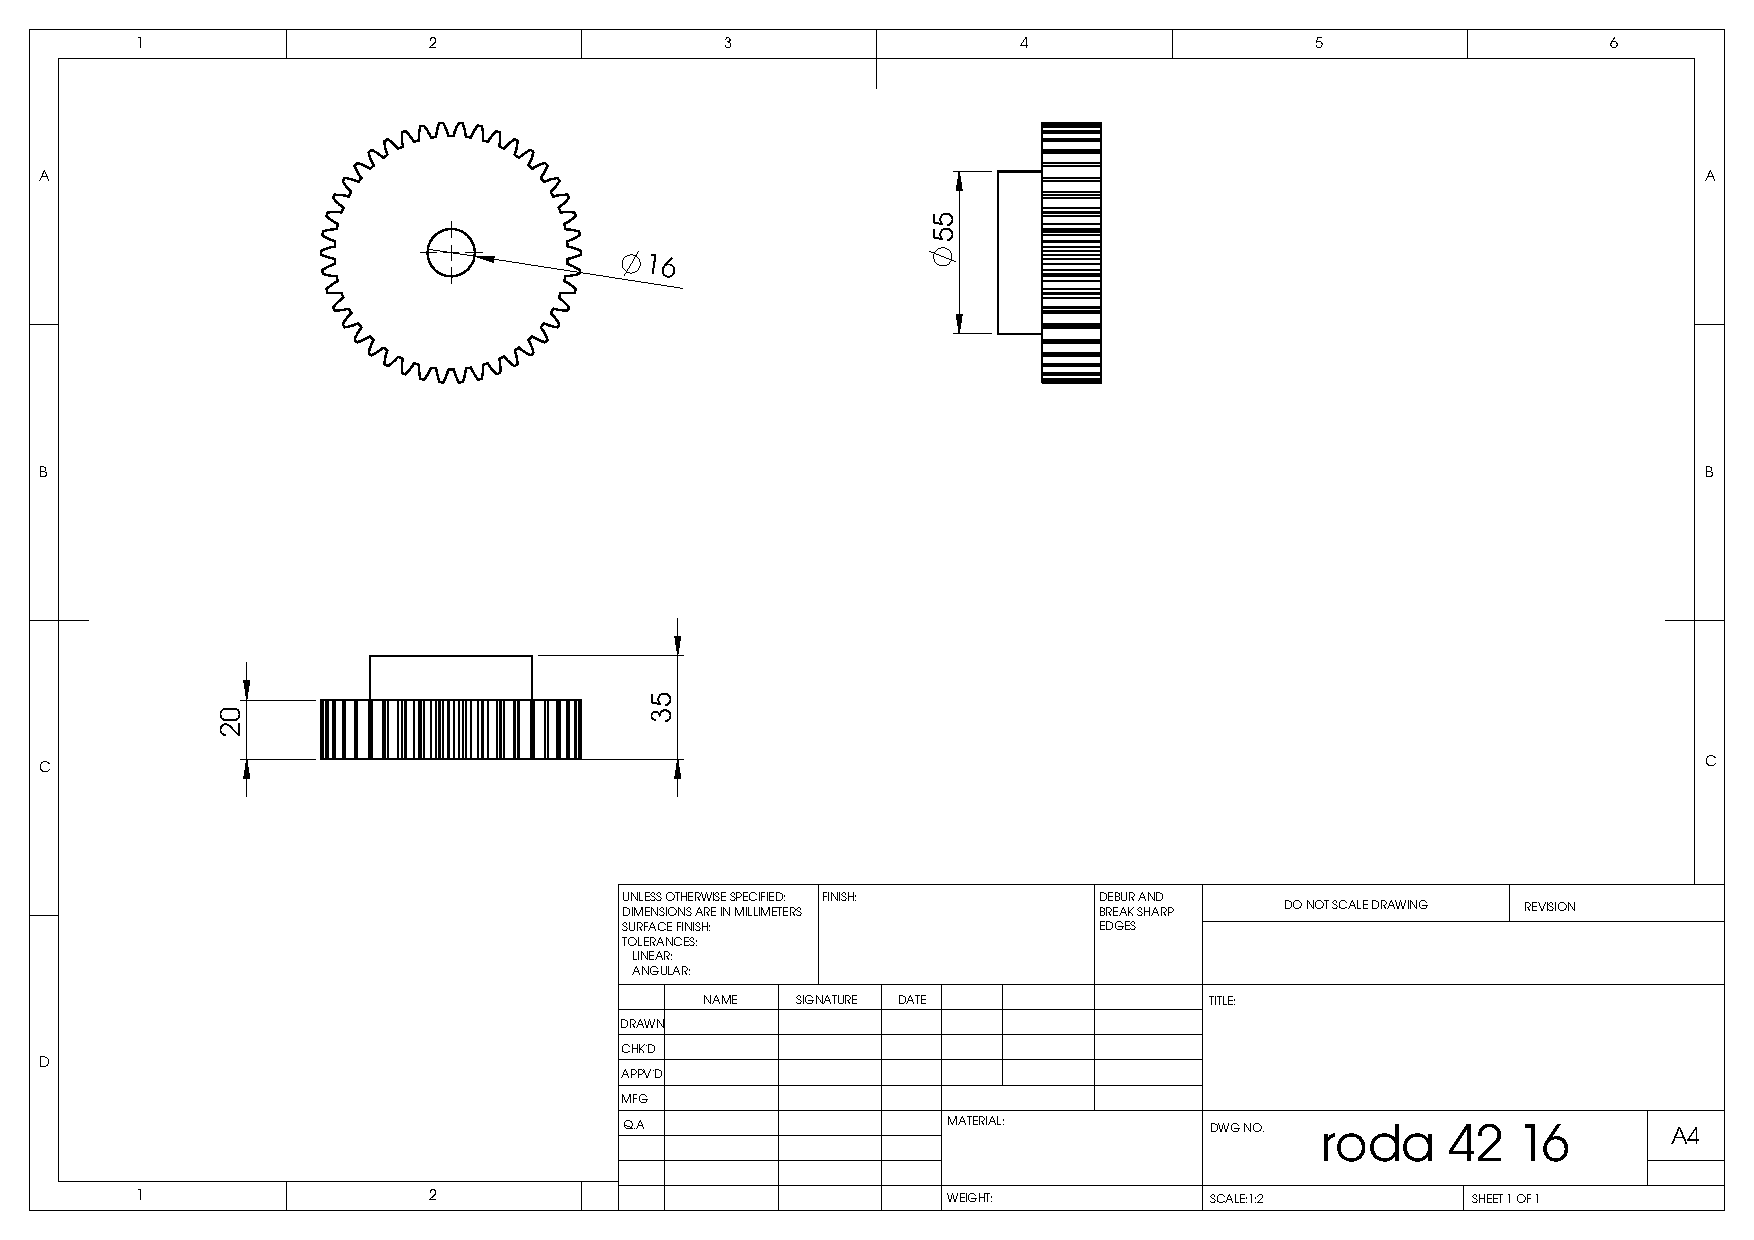
\includepdf[landscape=true]{recursos/esquemas/redutor_tracao_v1.0/engrenagem_z42_d16mm.pdf}
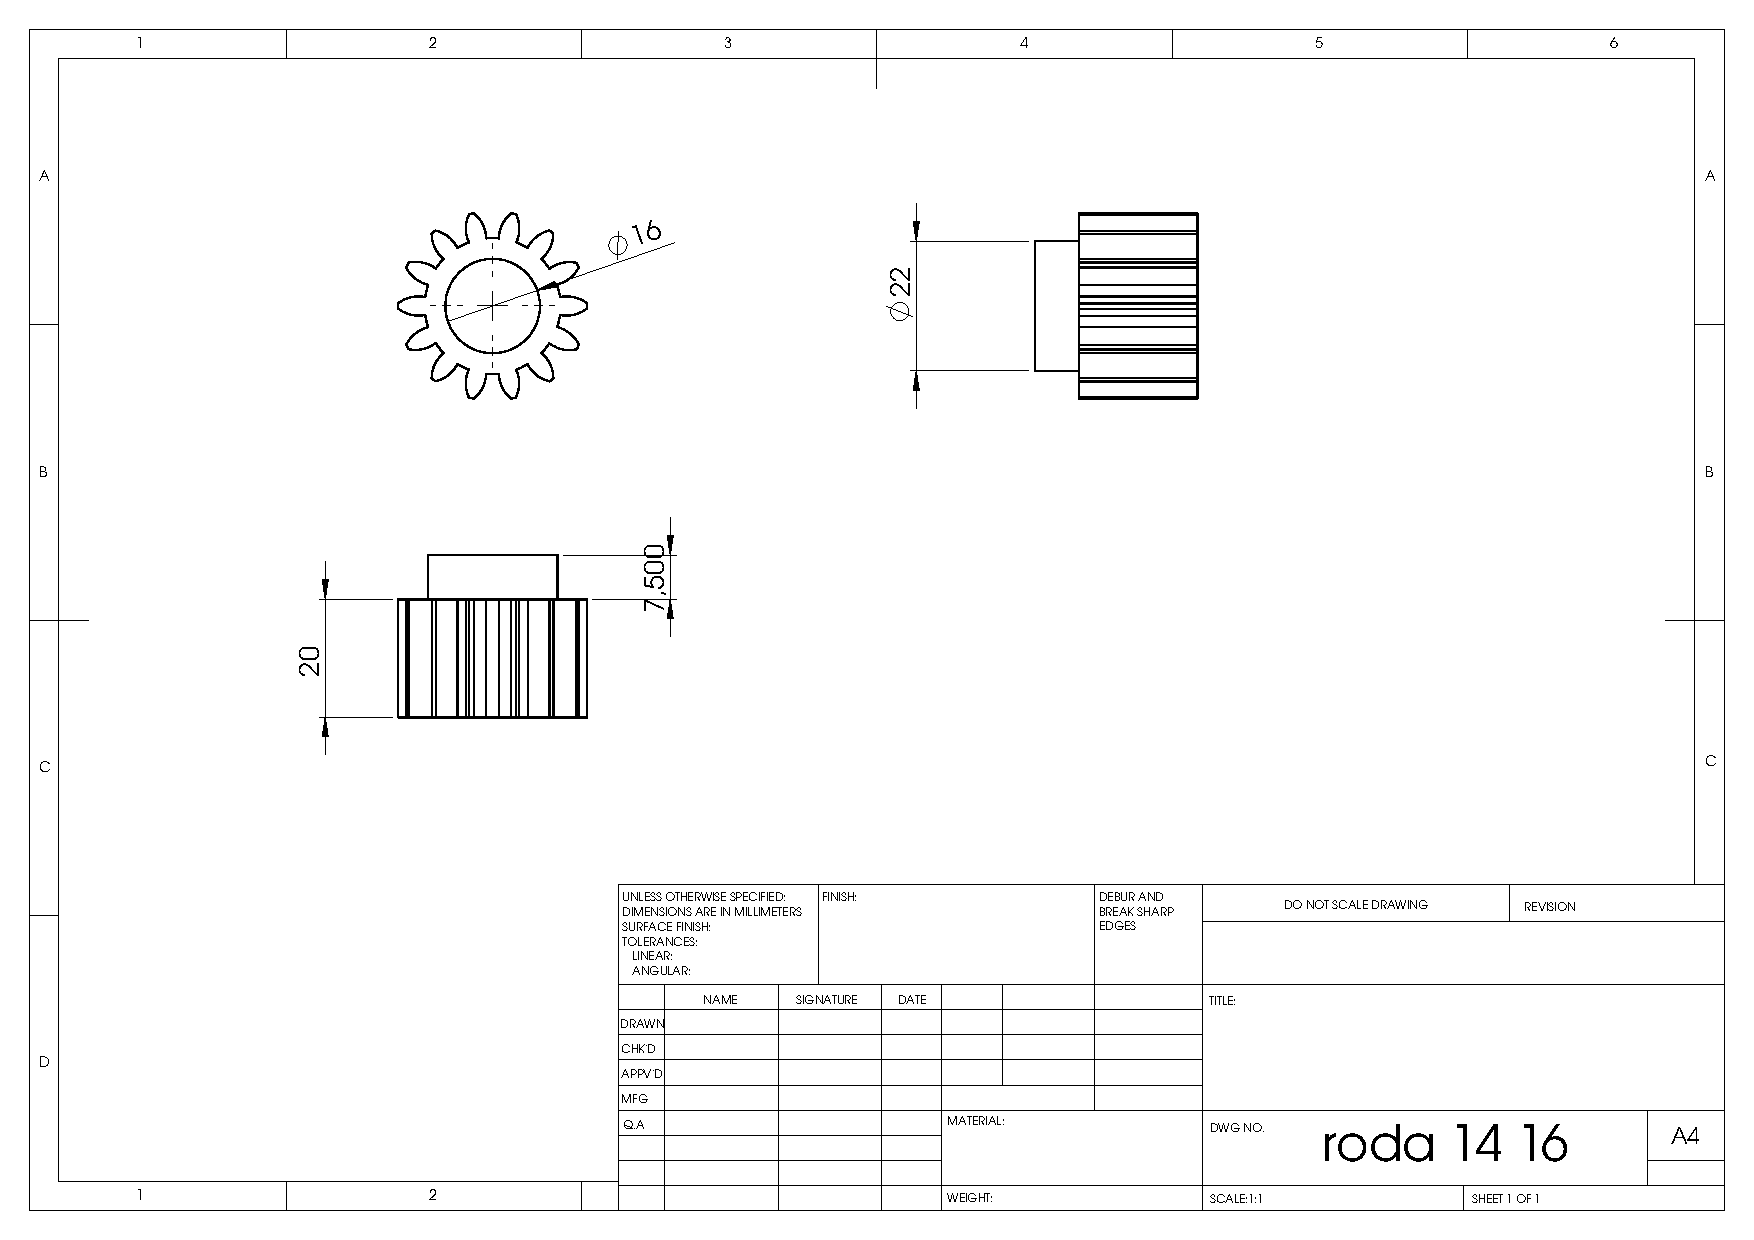
\includepdf[landscape=true]{recursos/esquemas/redutor_tracao_v1.0/engrenagem_z14.pdf}
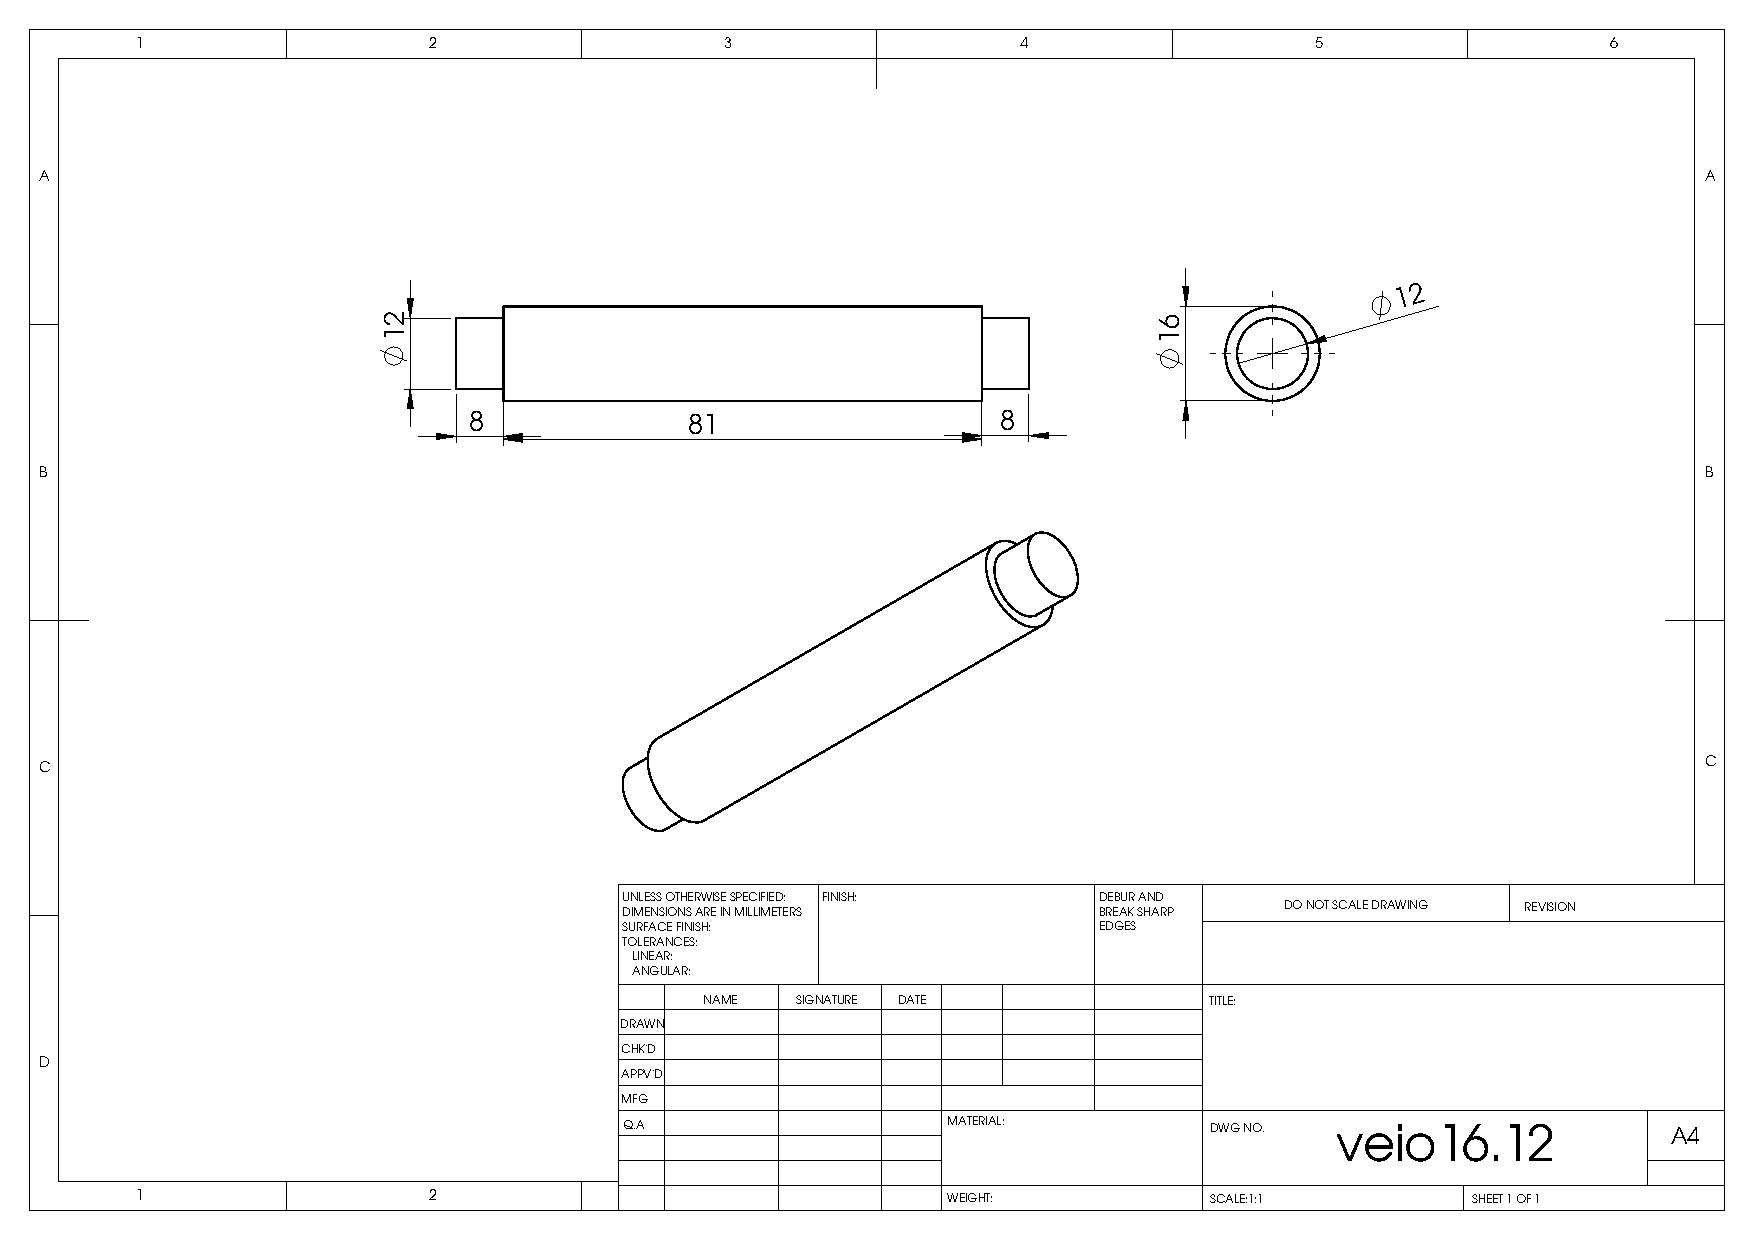
\includepdf[landscape=true]{recursos/esquemas/redutor_tracao_v1.0/veio_16_12mm.pdf}
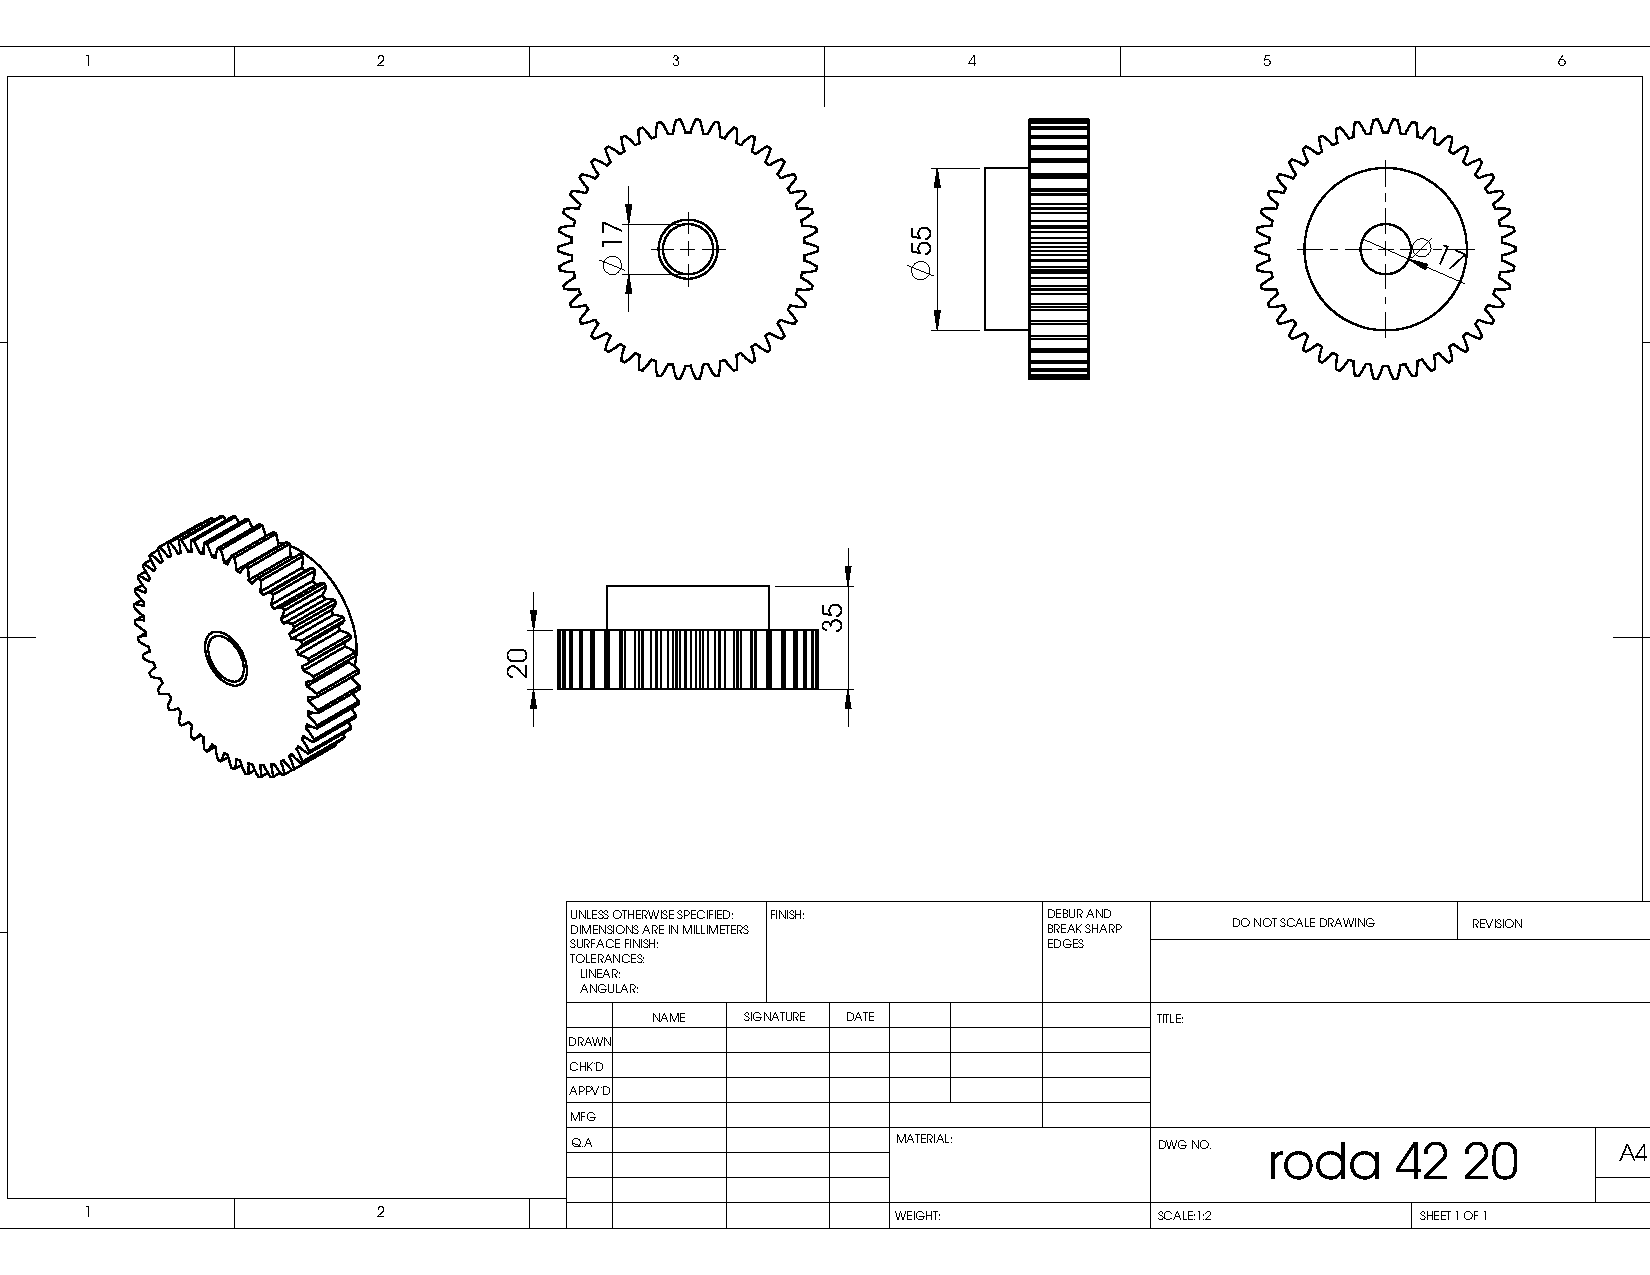
\includepdf[landscape=true]{recursos/esquemas/redutor_tracao_v1.0/engrenagem_z42_d17mm.pdf}
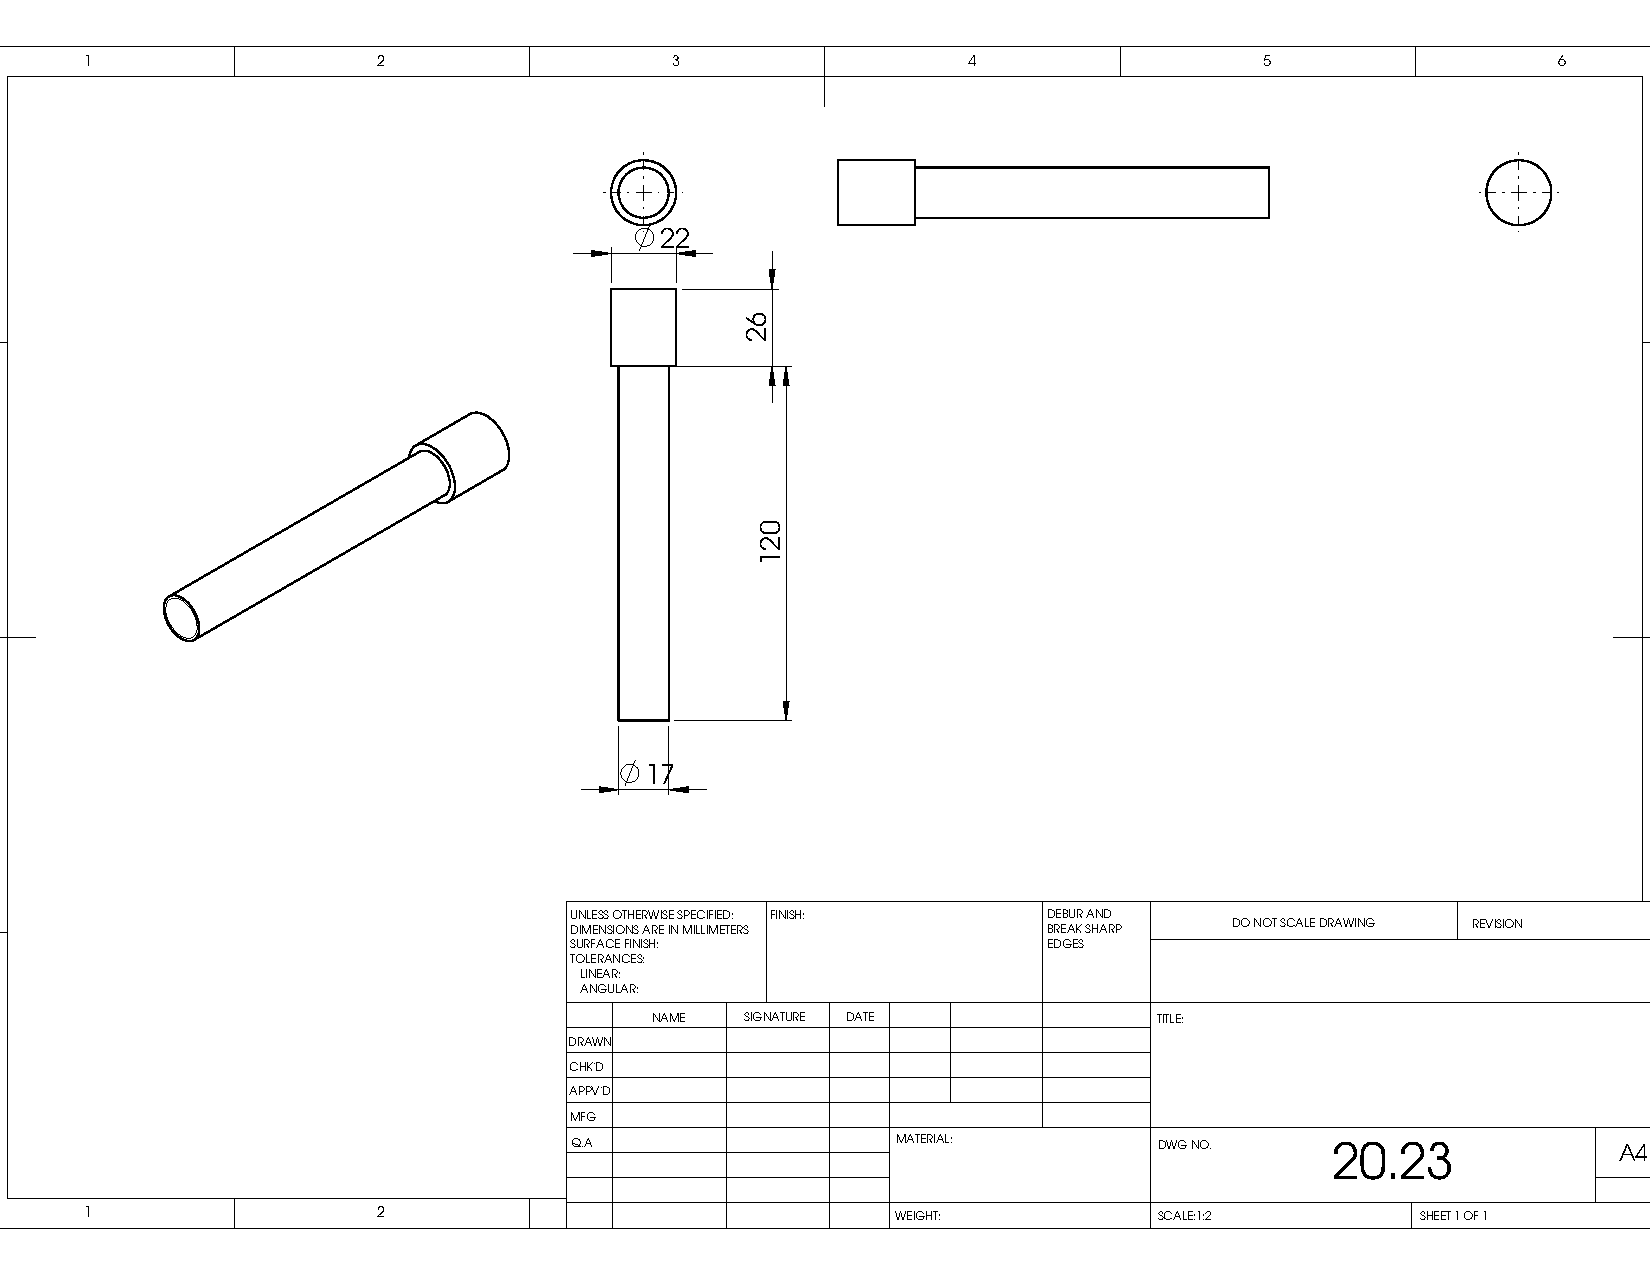
\includepdf[landscape=true]{recursos/esquemas/redutor_tracao_v1.0/veio_17_22mm.pdf}
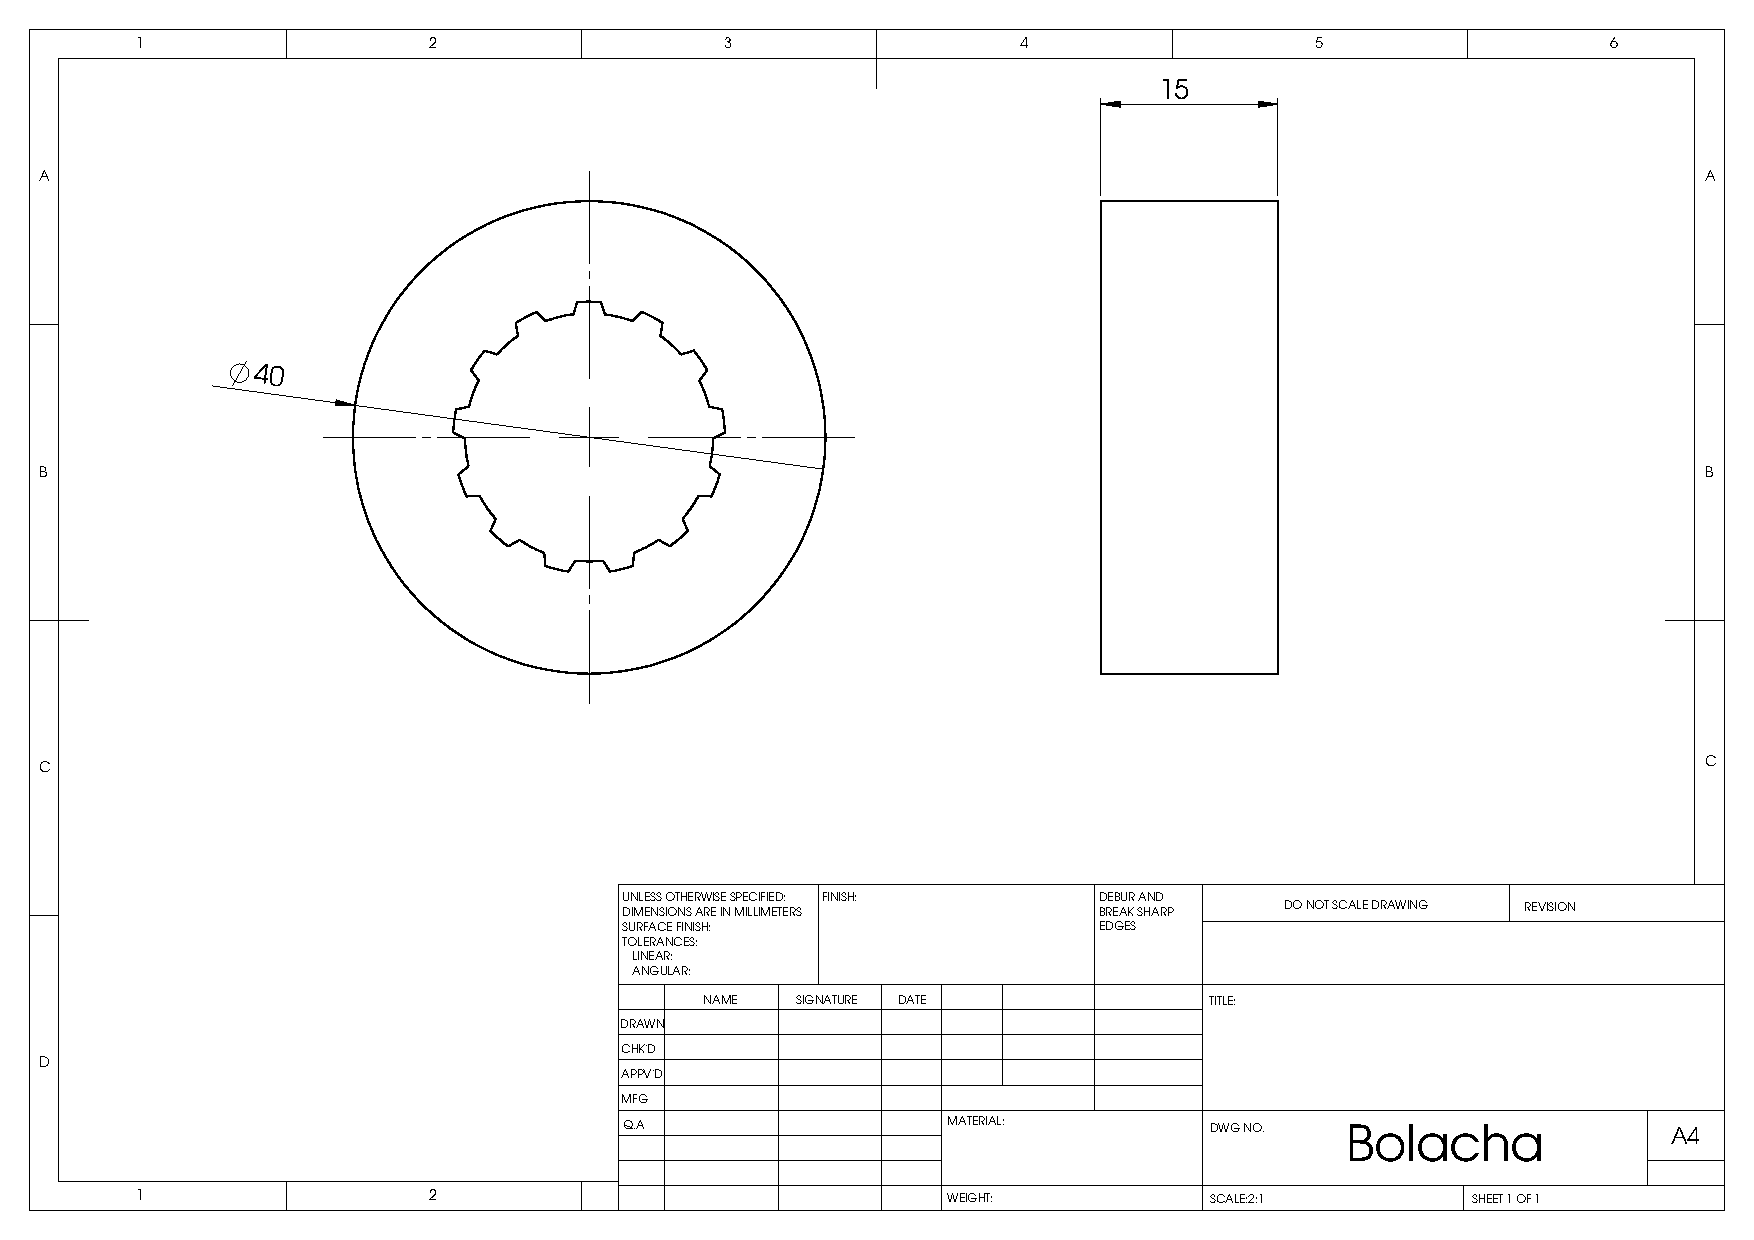
\includepdf[landscape=true]{recursos/esquemas/redutor_tracao_v1.0/bolacha_aperto_carreto.pdf}
Os desenhos deste anexo s�o uma especifica��o aproximada do redutor \emph{� priori}, com as limita��es inerentes � falta de experi�ncia do projetista. N�o contemplam alguns pormenores t�cnicos avan�ados, como toler�ncias nos encaixes, materiais a usar, e mecanismos de fixa��o. Como tal, o fabricante fez algumas modifica��es, discutidas na errata
\section*{Informa��es sobre o fabricante}
\raggedright\textbf{Vitor Ferreira \& Filhos, Lda}\\
Rua Particular � Rua Arco do Carvalh�o, Letras J.F.C, 1070 Lisboa\\
Telefone: 213884764\\
\url{www.mestredosmotores.com}
\section*{Errata}
Errata referente aos desenhos das pe�as do redutor do motor de tra��o

%\todo[talking point]{Pq n�o alterei os desenhos em vez de fazer uma errata? Pq alguns par�metros foram mudados pelo torneiro durante a manufatura (ap�s o desenho da caixa), e document�-los implicaria desmontar parcialmente ou na totalidade a caixa...}
\todo{fazer as corre��es na errata e alterar o nome dos desenhos}
% If you want to place your tables where they lie in your source code and you do not need any label, do not use table at all!
\begin{center}
    %Tried using tabularx and tabulary, and both sucked - could not handle the extra large column well.
    \begin{tabular}{b{0.15\textwidth} b{0.15\textwidth} b{0.6\textwidth}}
        \textbf{Desenho} & \textbf{Onde se l�/v�} & \textbf{Deve l�r-se/v�r-se}\\ \midrule
        espa�ador chapa & 85 & 87\\
        roda 21 & R10 & R9.5\\
        roda 21 & 12.800 & 12.300\\
        roda 21 & & Chave (paralelip�pedo quadrangular com 6 mm de lado, cantos arredondados e 35 mm de comprimento) para prender engrenagem de 21 dentes ao veio do motor, de acordo com a norma ISO/R773 \cite{norma_ISO_R773}.\\
        20.23 & Face do veio \diameter22 liso & Face do veio \diameter22 liso at� 11mm ap�s o \diameter17. Da� at� ao topo, veio maquinado para encaixe no buraco da bolacha do desenho "bolacha".\todo[talking point]{com a largura do carreto, a bolacha n�o entra totalmente no veio.}\\
        20.23 & Topo do veio \diameter22 liso & Topo do veio \diameter22 com rosca M8 conc�ntrica.\\
        20.23 & 120 & 115, medidos a partir do veio \diameter22. Ranhura para freio ap�s a medida.\done\todo{confirmar}\\
        bolacha & & Um dos topos do cilindro tapado, com um furo M8 conc�ntrico.\\
        chapa corrente & 12 furos de 4 mm & 4 furos M10 pr�ximos dos cantos da placa.\\
        chapa motor & 12 furos de 4 mm & 4 furos M10 pr�ximos dos cantos da placa, � mesma dist�ncia dos da errata do desenho "chapa corrente".\\
        montagem & Veio do motor & Espa�ador cil�ndrico com furo conc�ntrico de 19 mm e cerca de 3 mm de largura, montado no veio, antes da engrenagem.\\
    \end{tabular}
\end{center}

        
\fancychapter{Ap�ndice F - Fotografias}
\label{ap:f}

%Neste ap�ndice s�o apresentas fotografias adicionais, tiradas ao longo da constru��o da \ac{T2D}.
\clearpage

%\begin{figure}[H]
%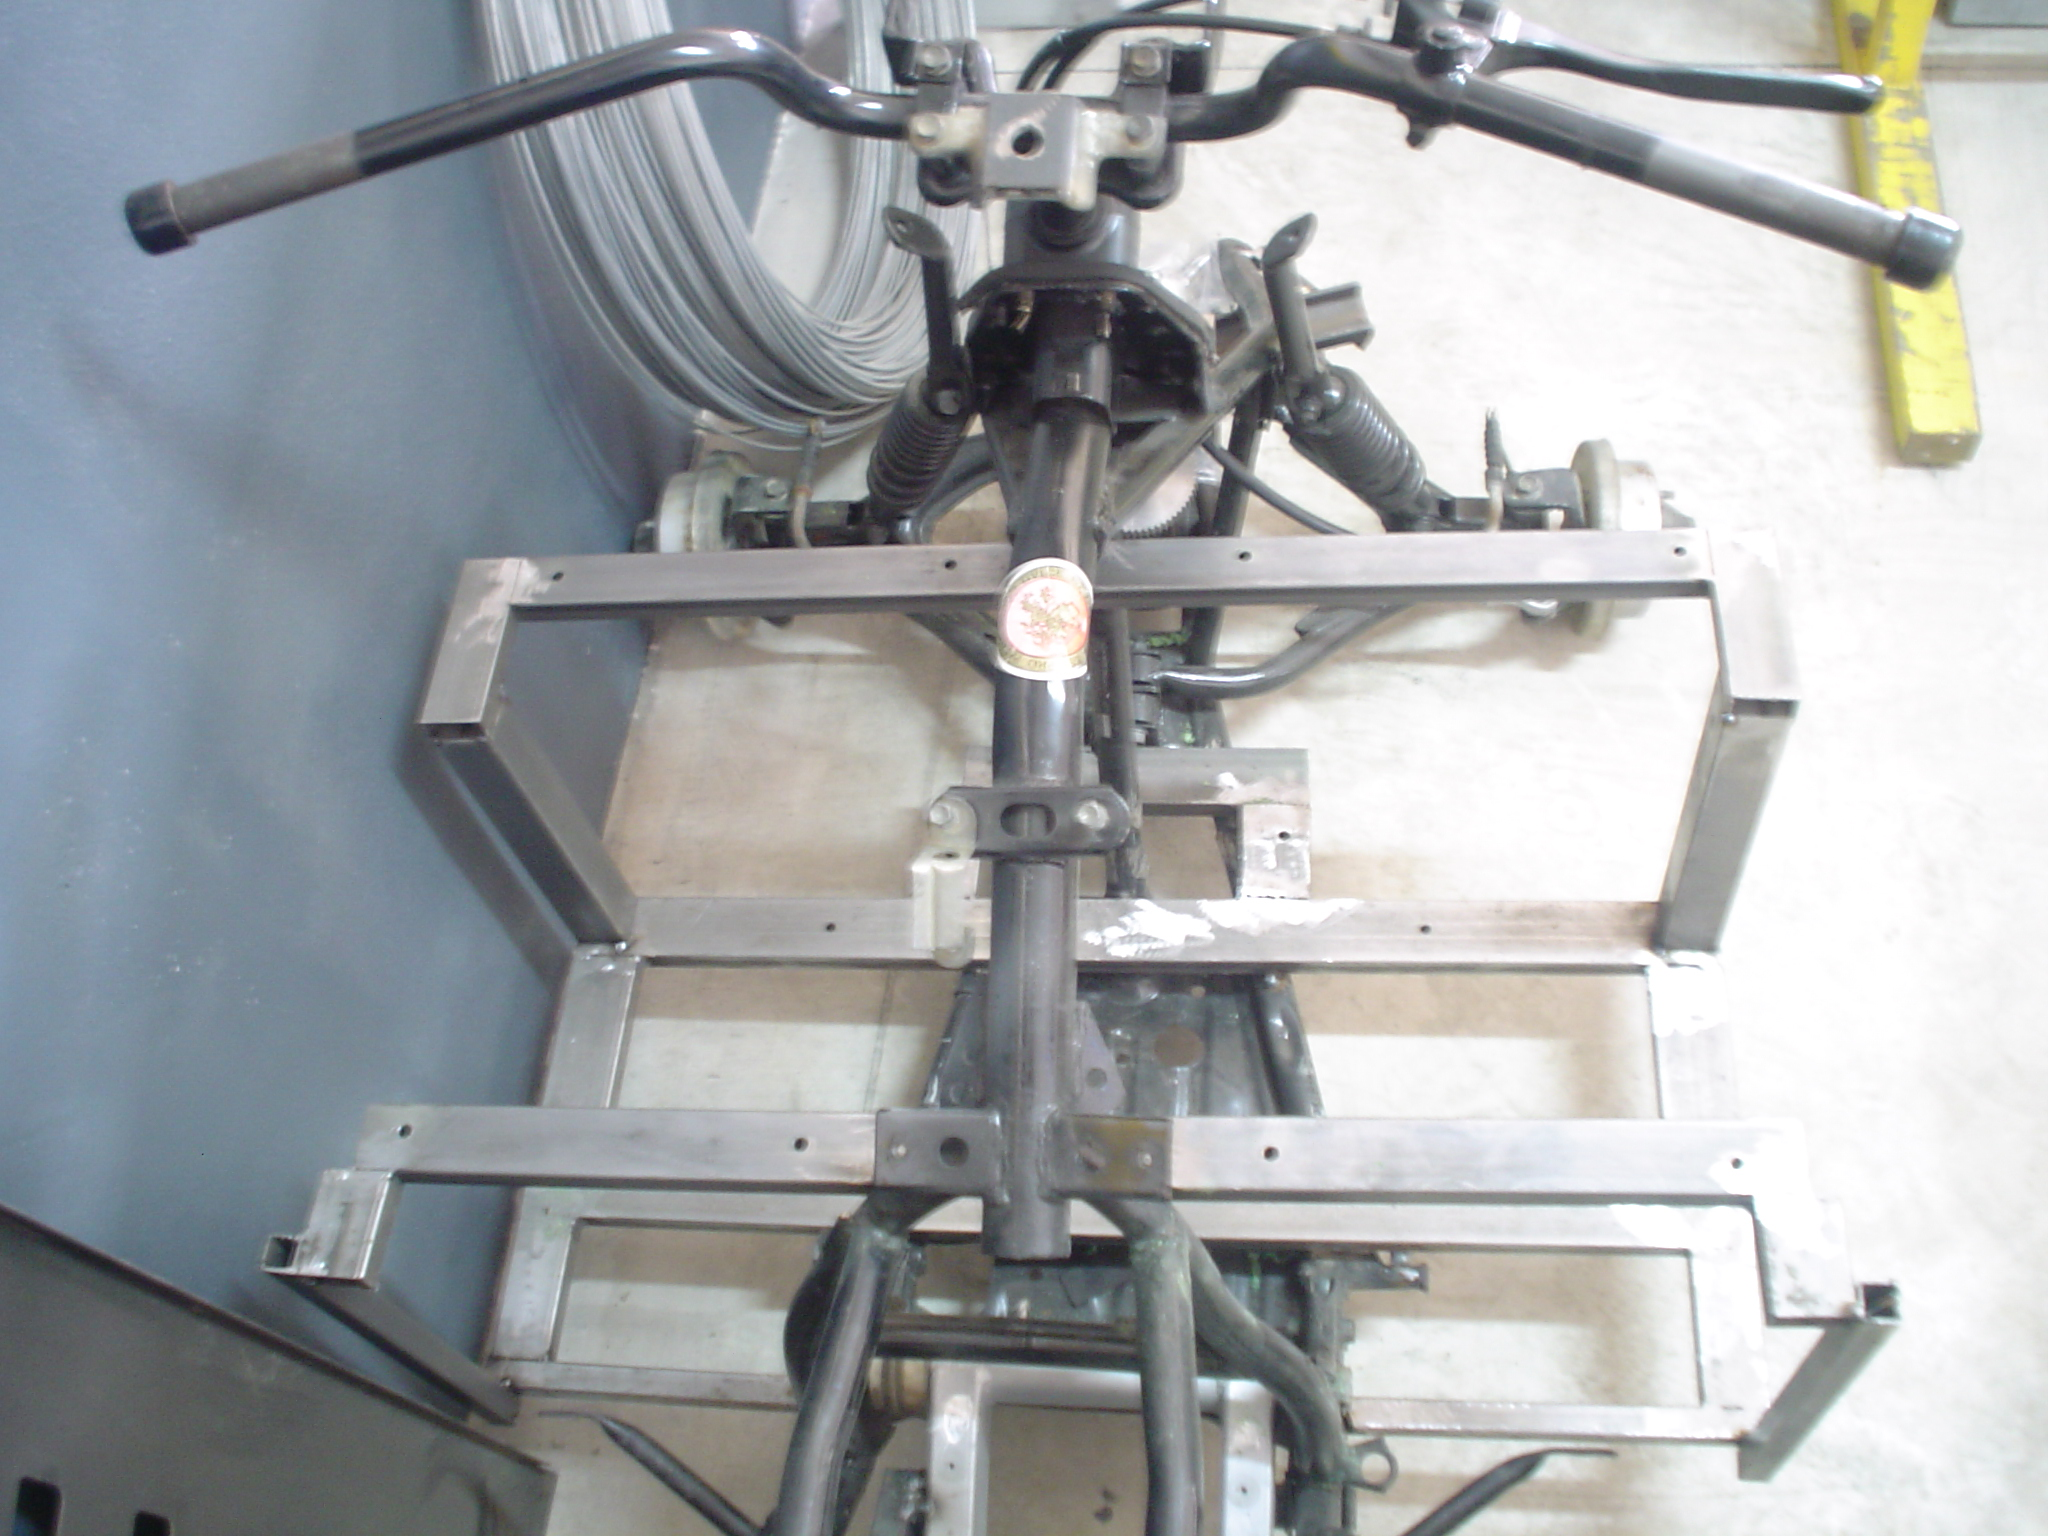
\includegraphics[width=\linewidth]{recursos/imagens/apendicef/chassi_baia_baterias} 
%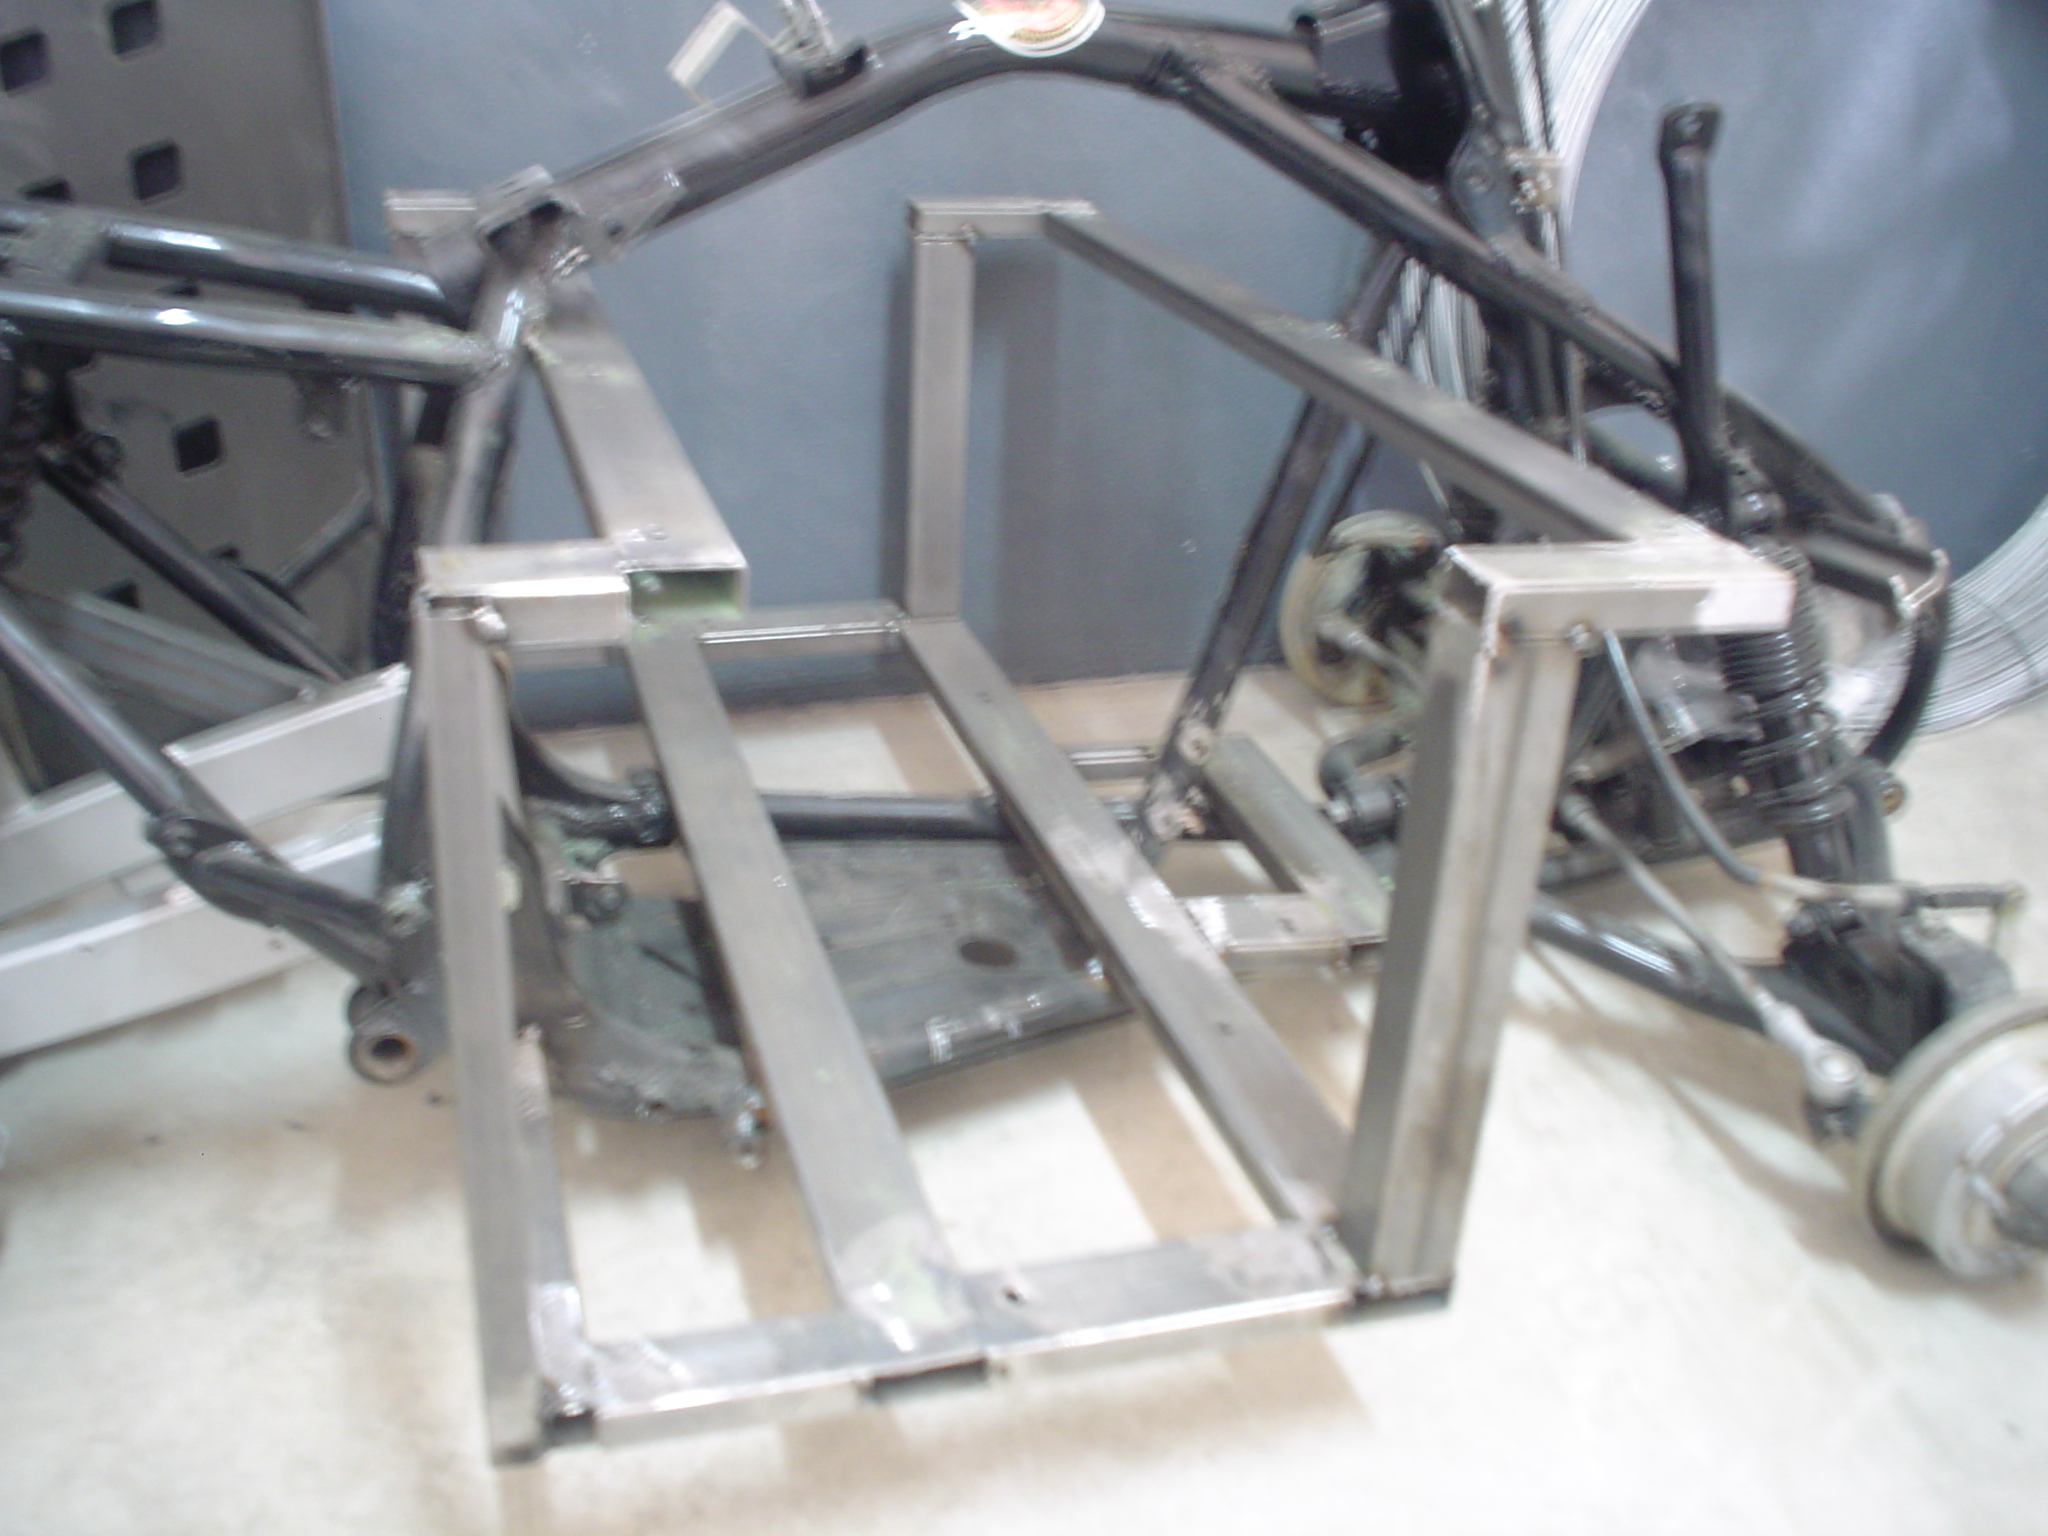
\includegraphics[width=\linewidth]{recursos/imagens/apendicef/chassi_estrutura_plataformas}
%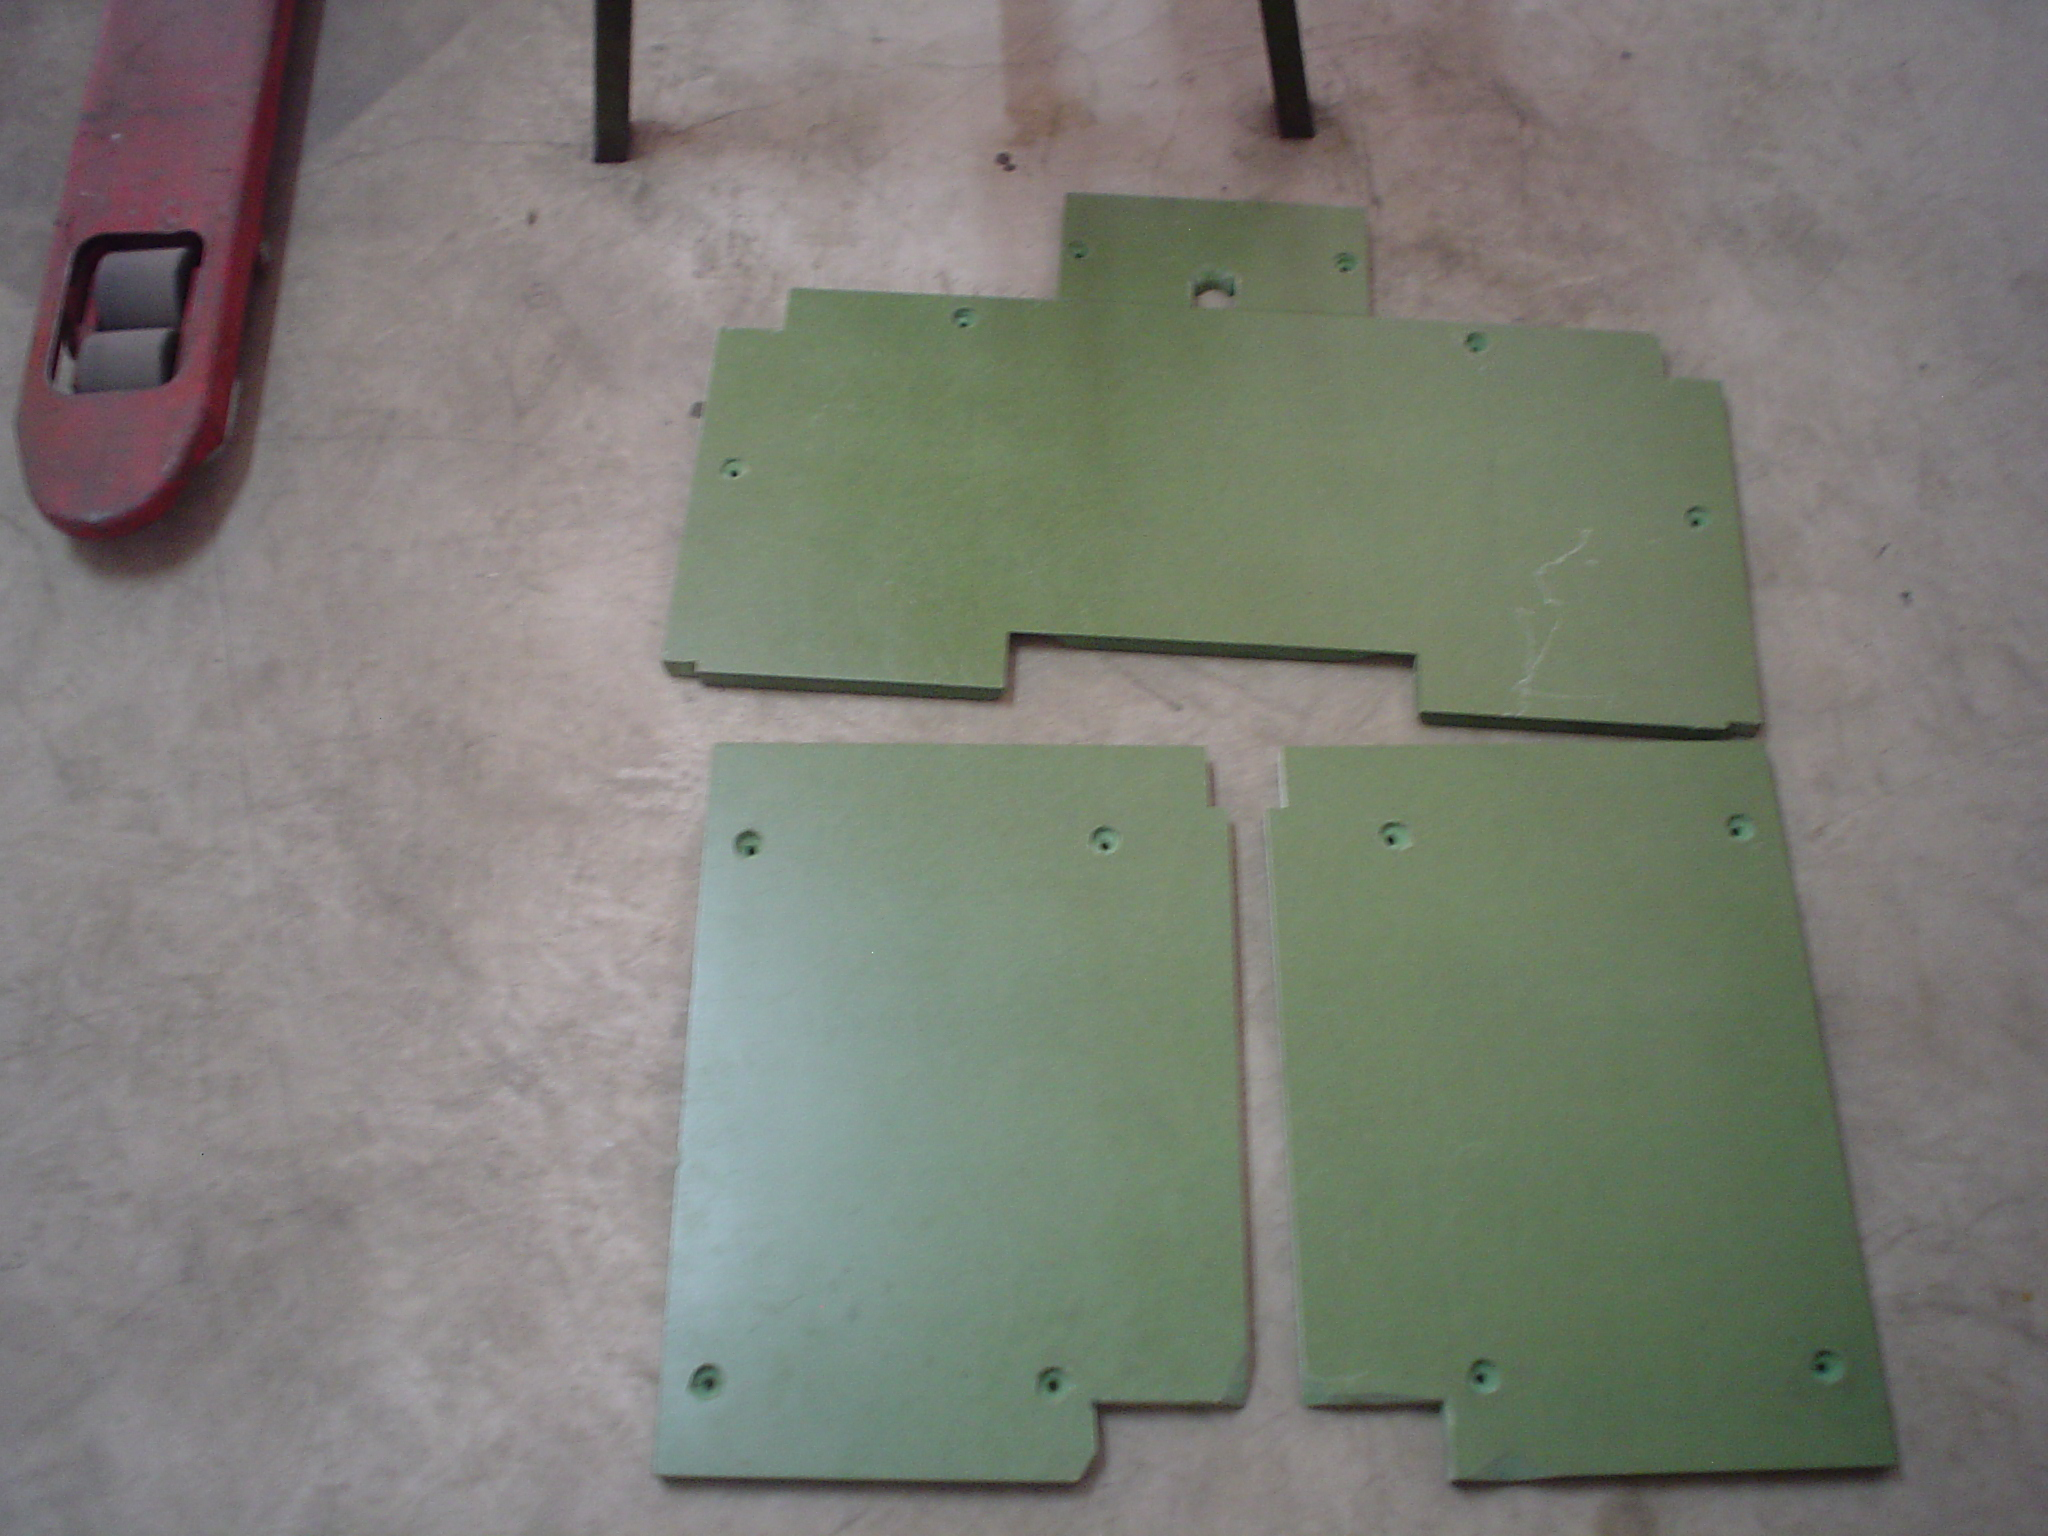
\includegraphics[width=\linewidth]{recursos/imagens/apendicef/chassi_madeira_plataformas} 
%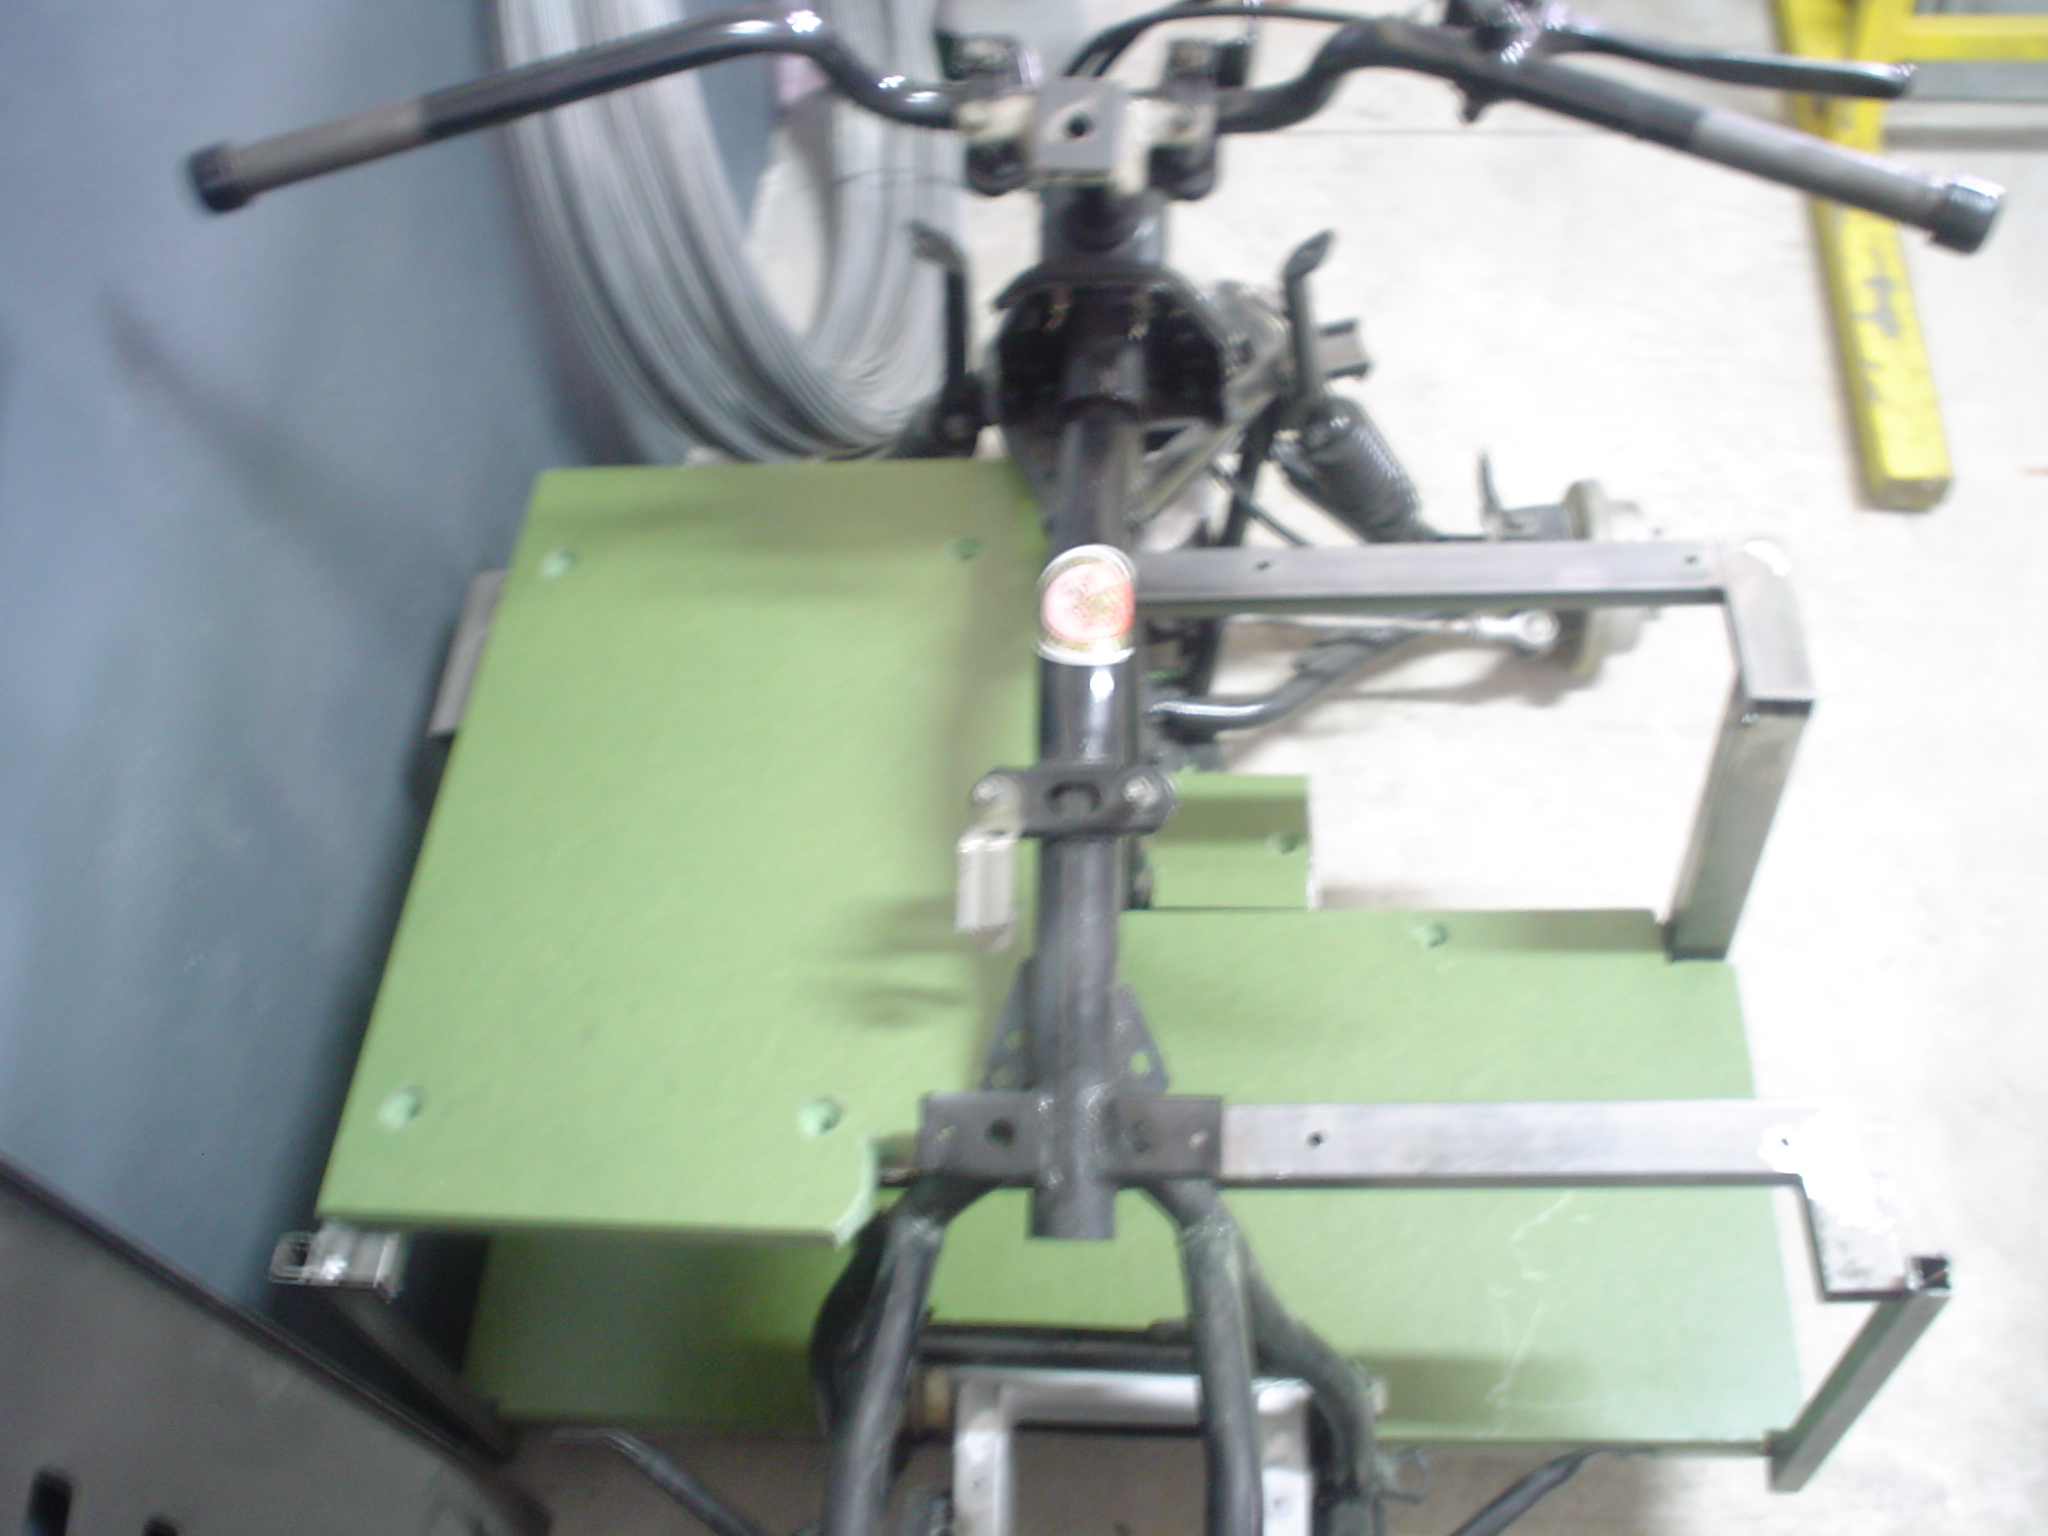
\includegraphics[width=\linewidth]{recursos/imagens/apendicef/chassi_plataformas} 
%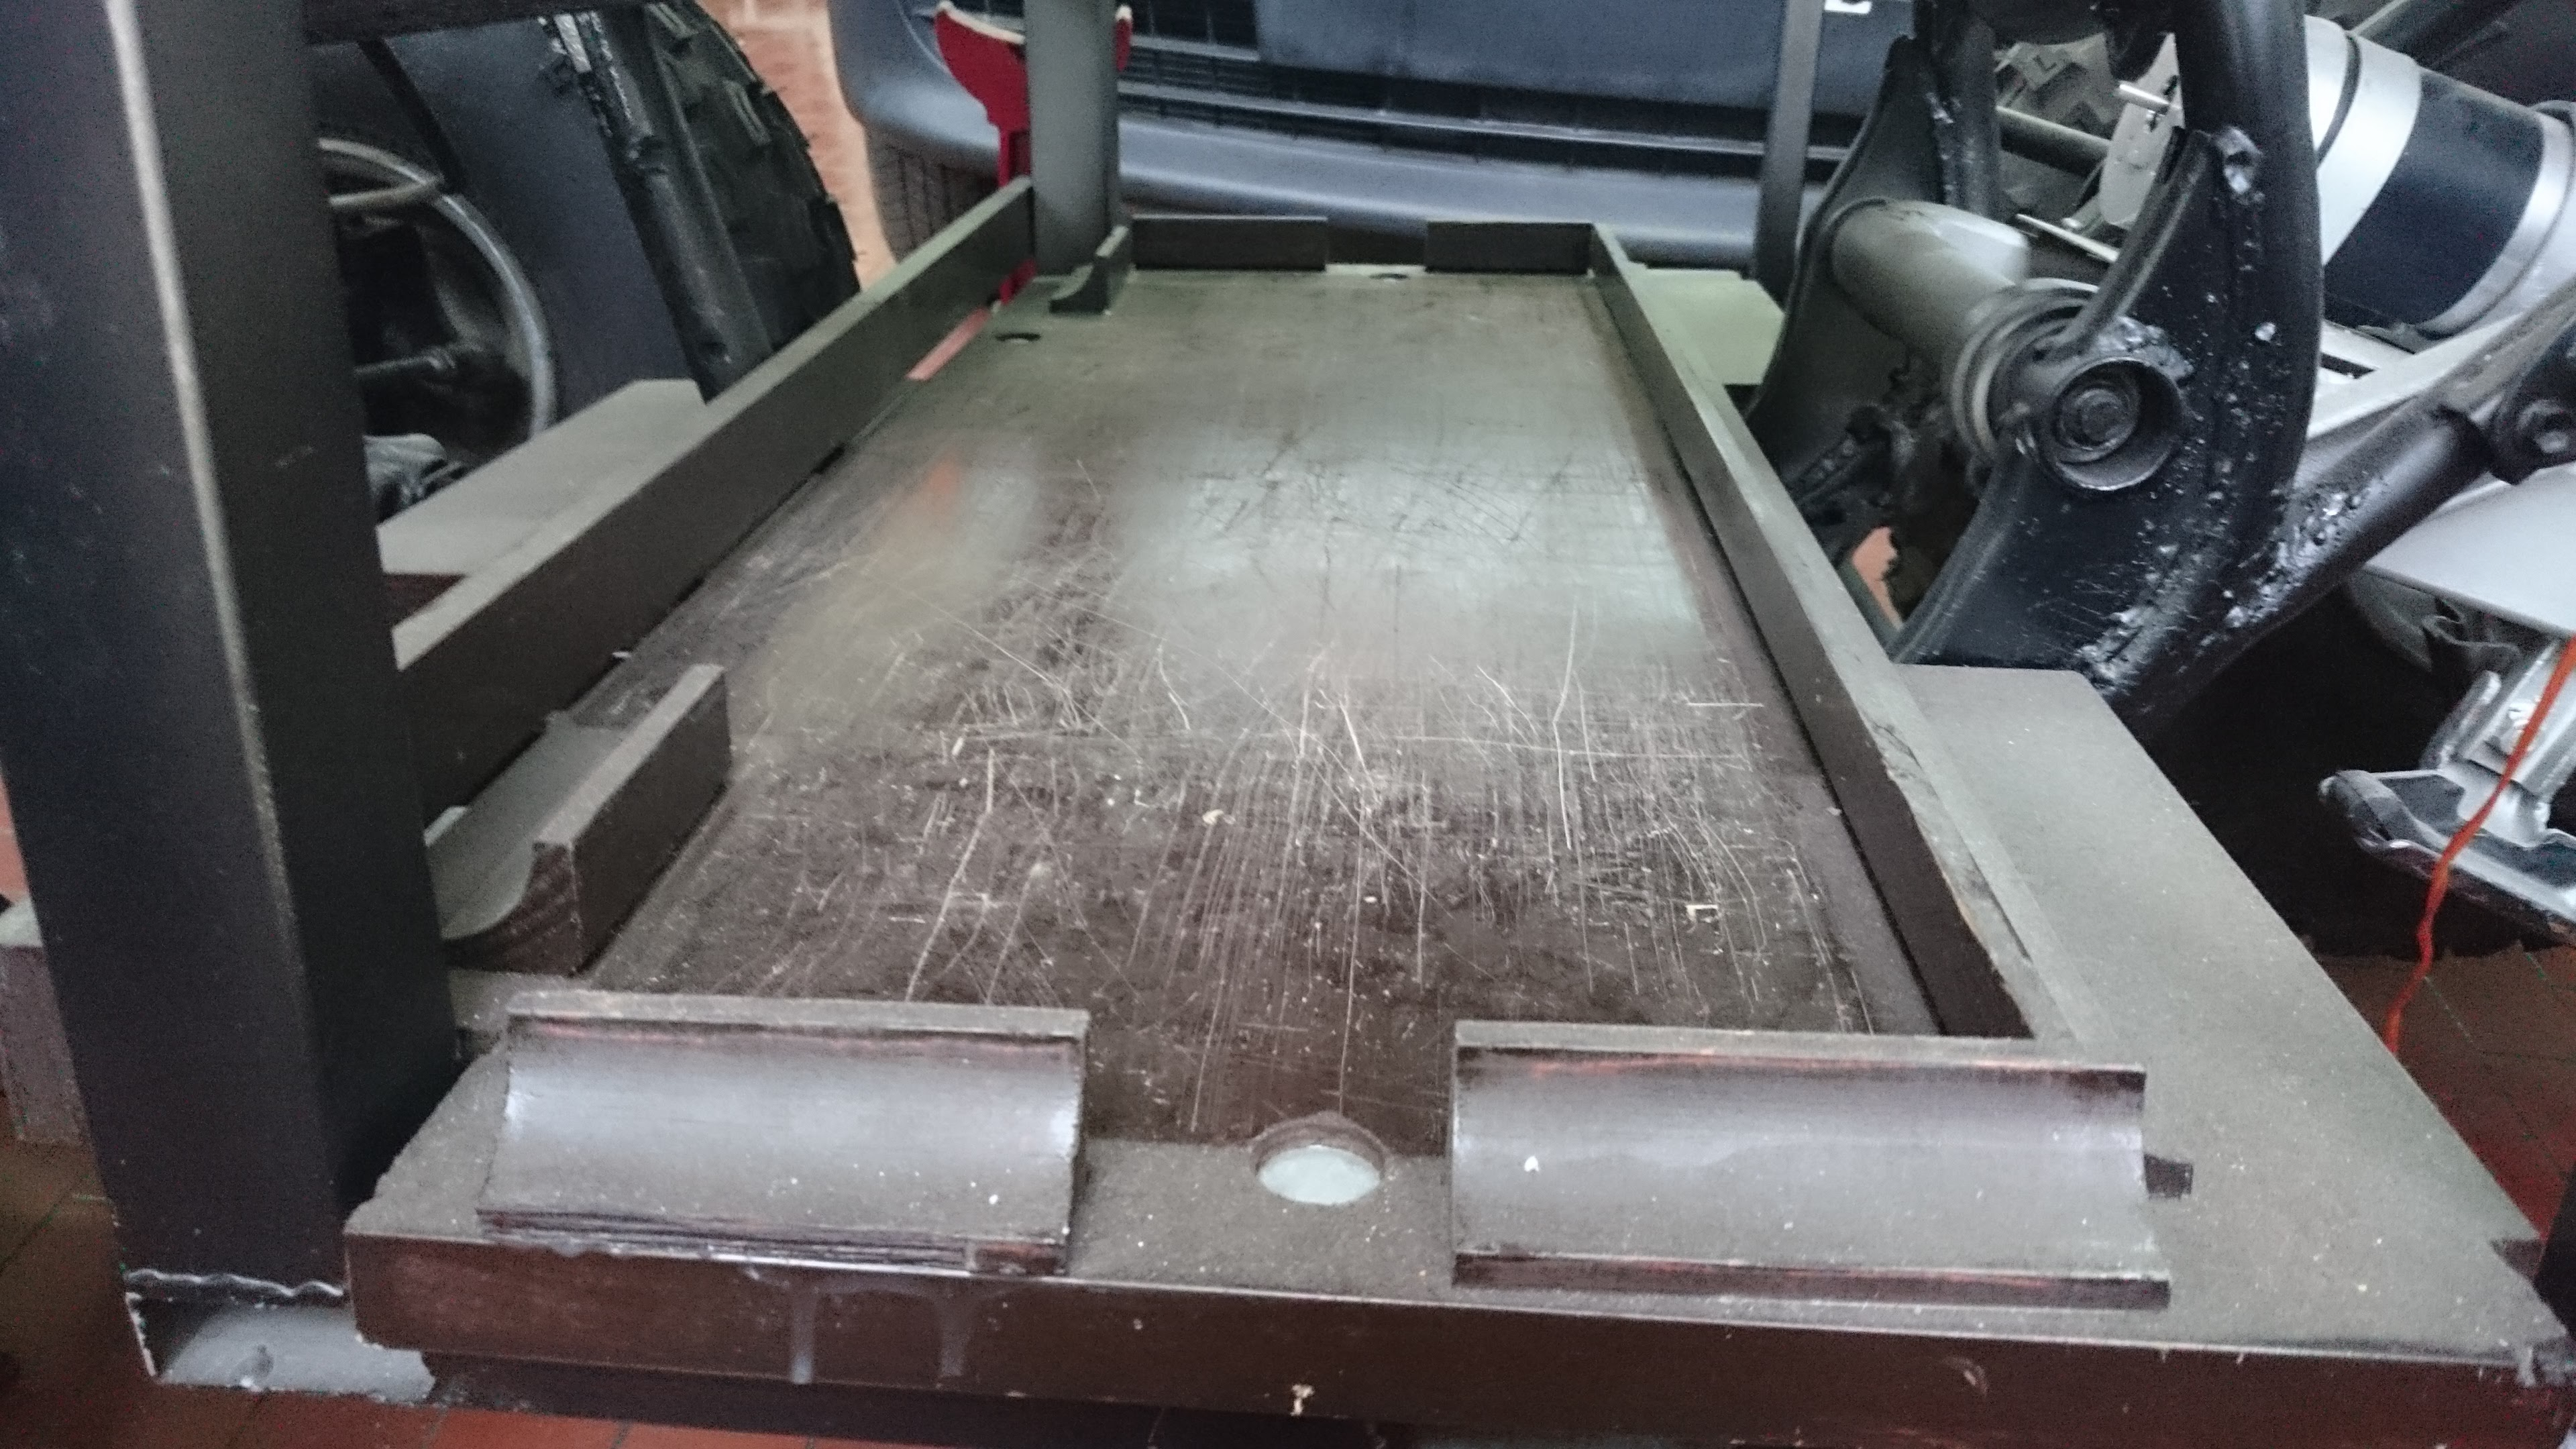
\includegraphics[width=\linewidth]{recursos/imagens/apendicef/chassi_plataforma_inferior} 
%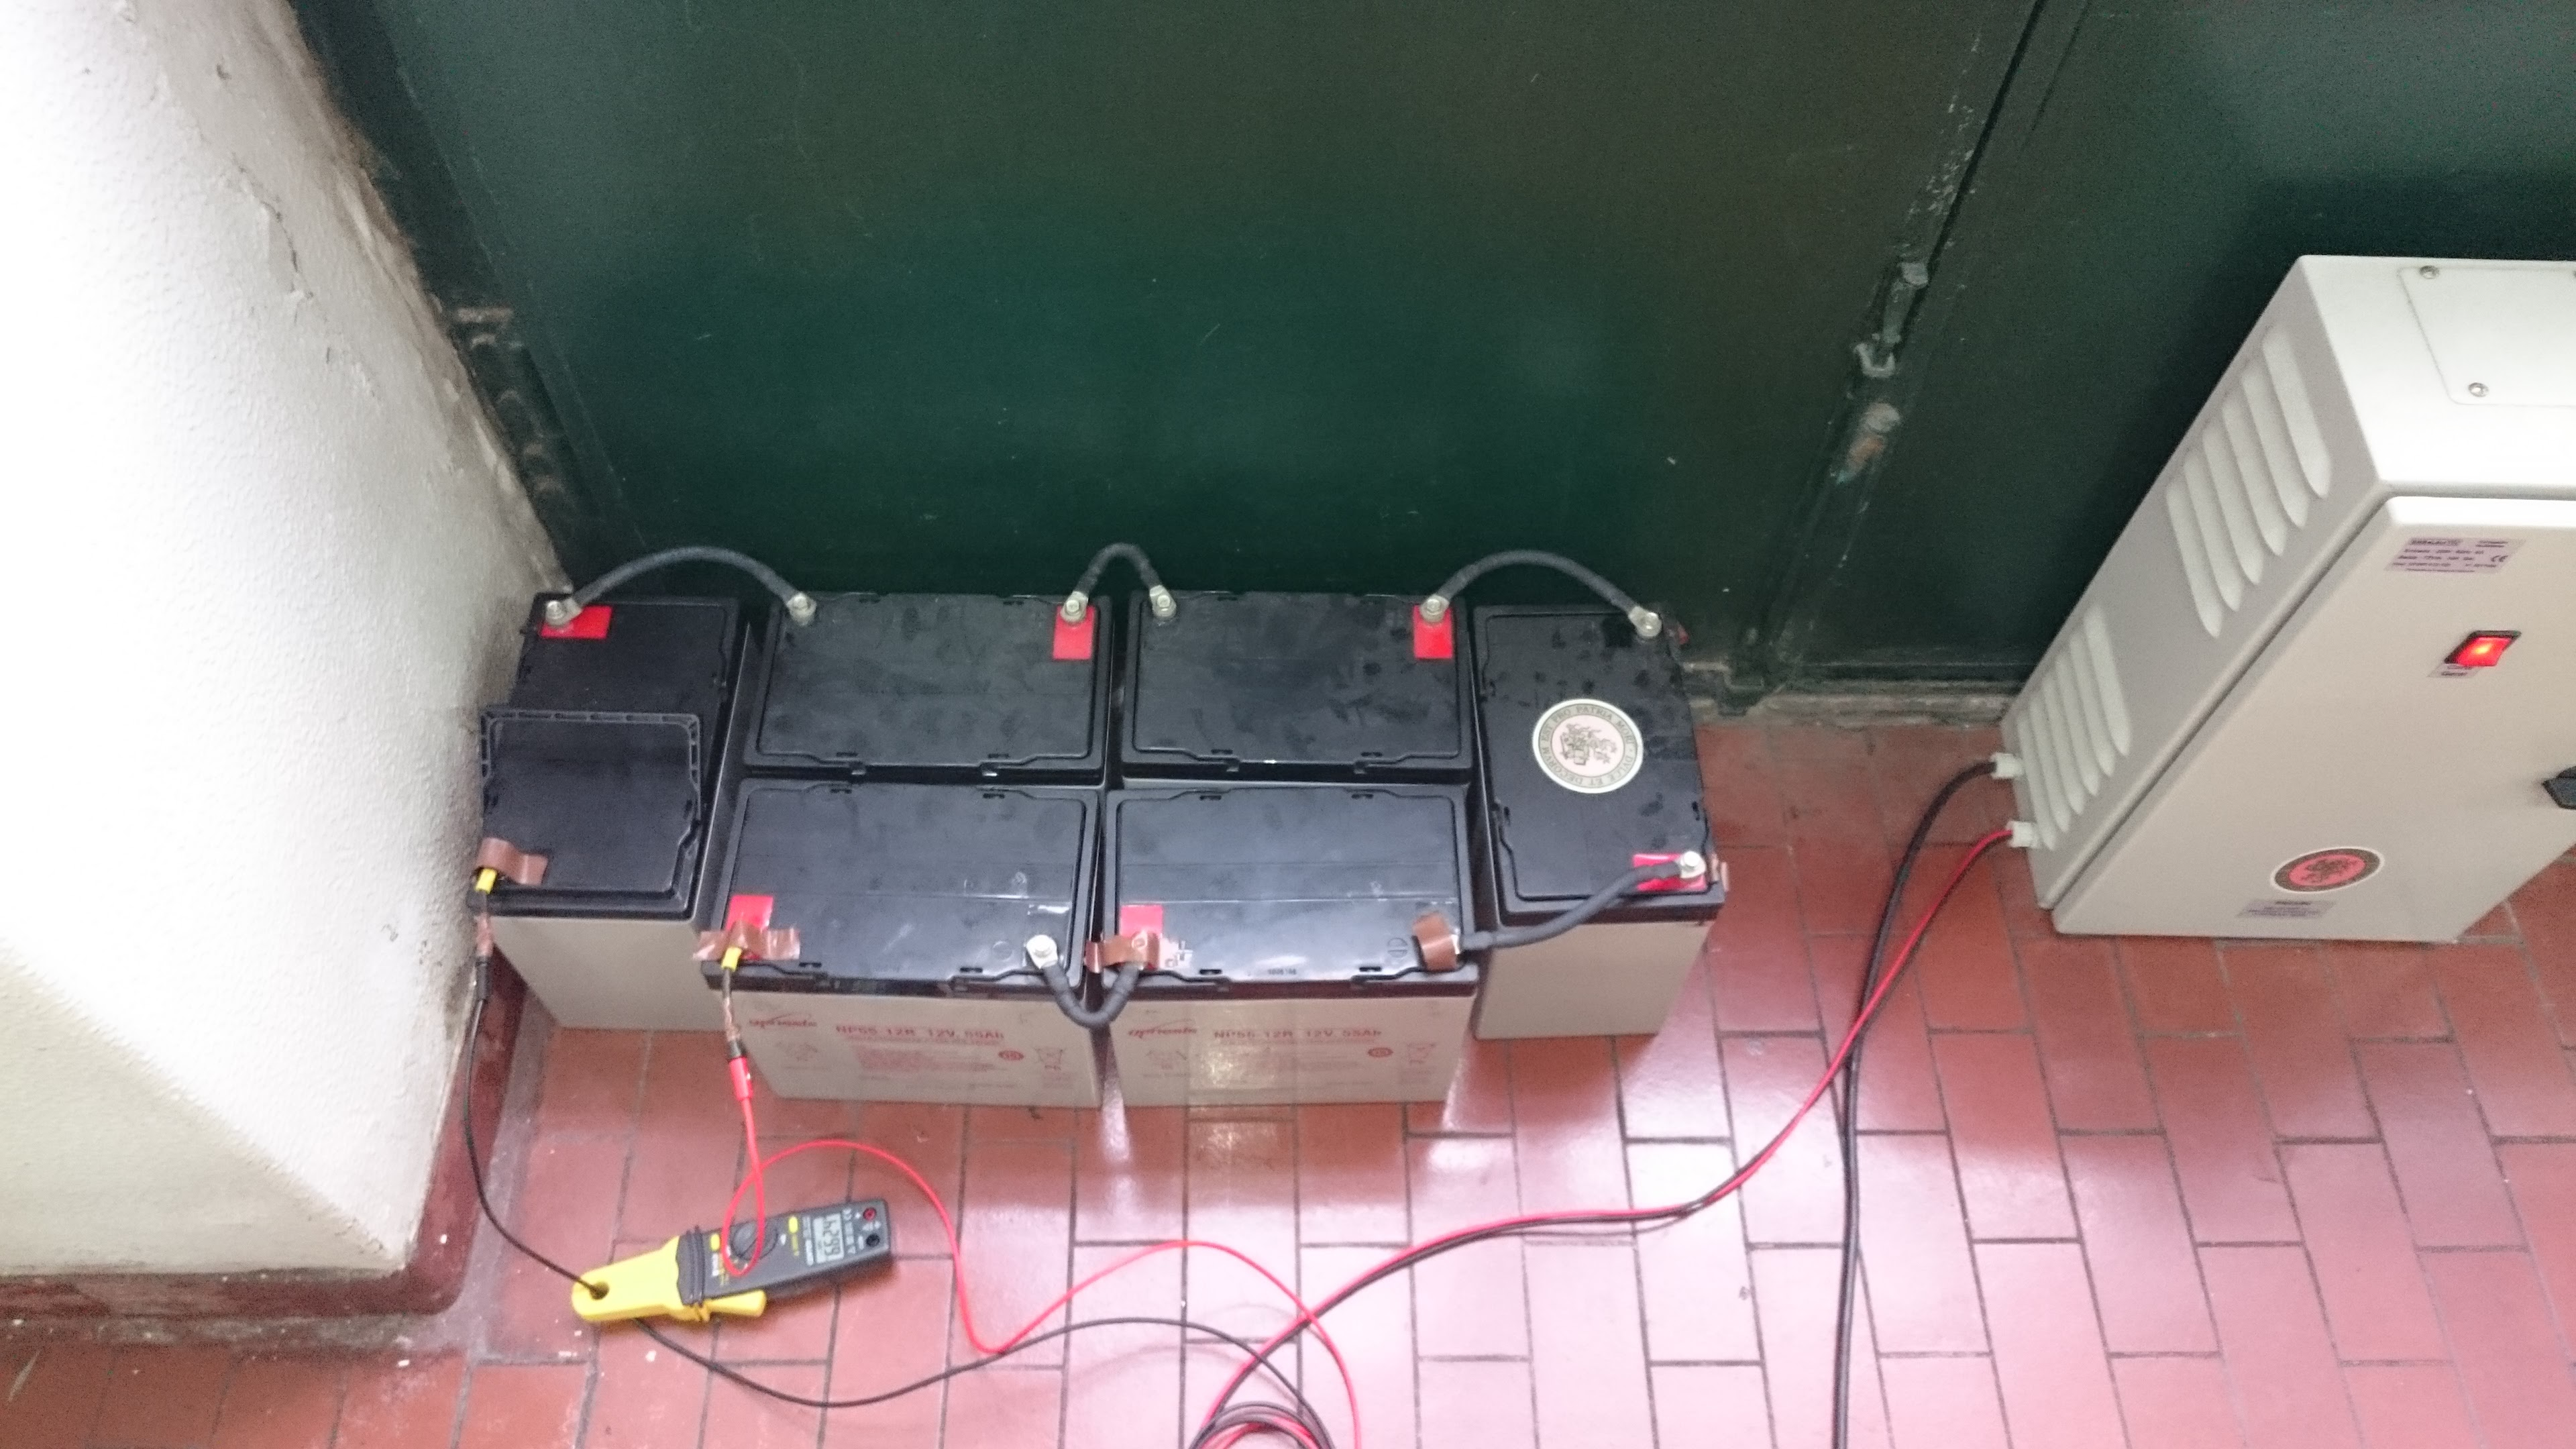
\includegraphics[width=\linewidth]{recursos/imagens/apendicef/bateria_carregando} 
%\end{figure}

\begin{figure}
\centering
\begin{subfigure}[b]{.45\linewidth}
    \subcaptionbox{Estrutura das plataformas no \emph{chassi}, vista de cima.\label{fig:chassi_estrutura_cima}}{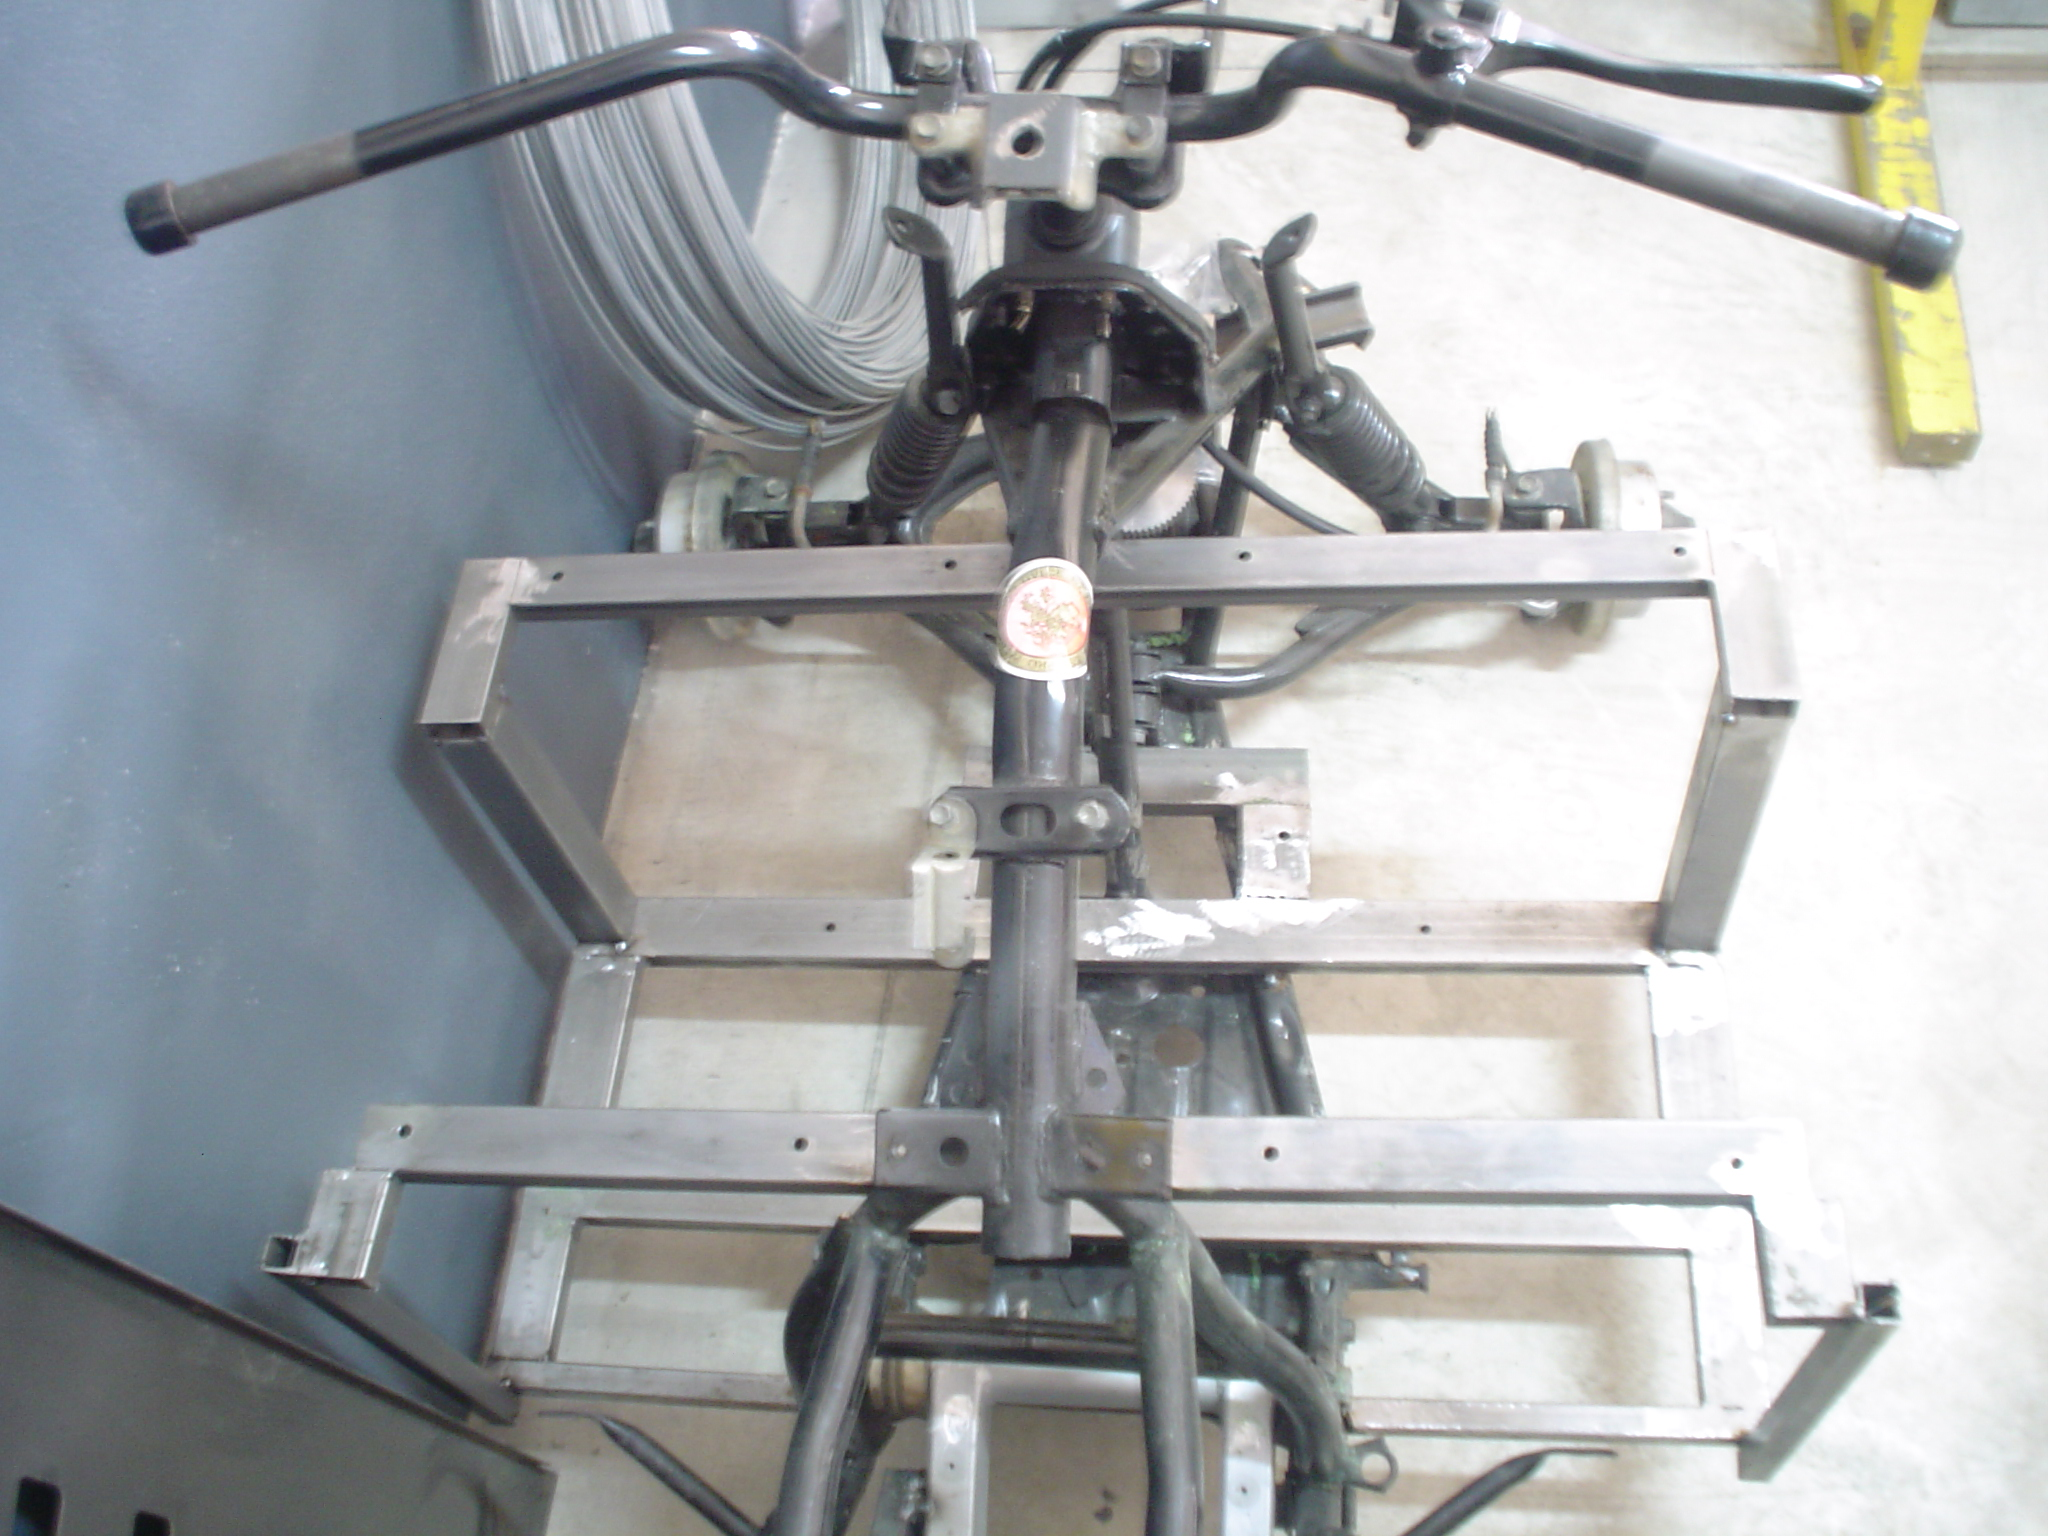
\includegraphics[width=\linewidth]{recursos/imagens/apendicef/chassi_baia_baterias.jpg} }
\end{subfigure}
\qquad
\begin{subfigure}[b]{.45\linewidth}
    \subcaptionbox{Estrutura das plataformas no \emph{chassi}, vista de lado.    \label{fig:chassi_estrutura_lado}}{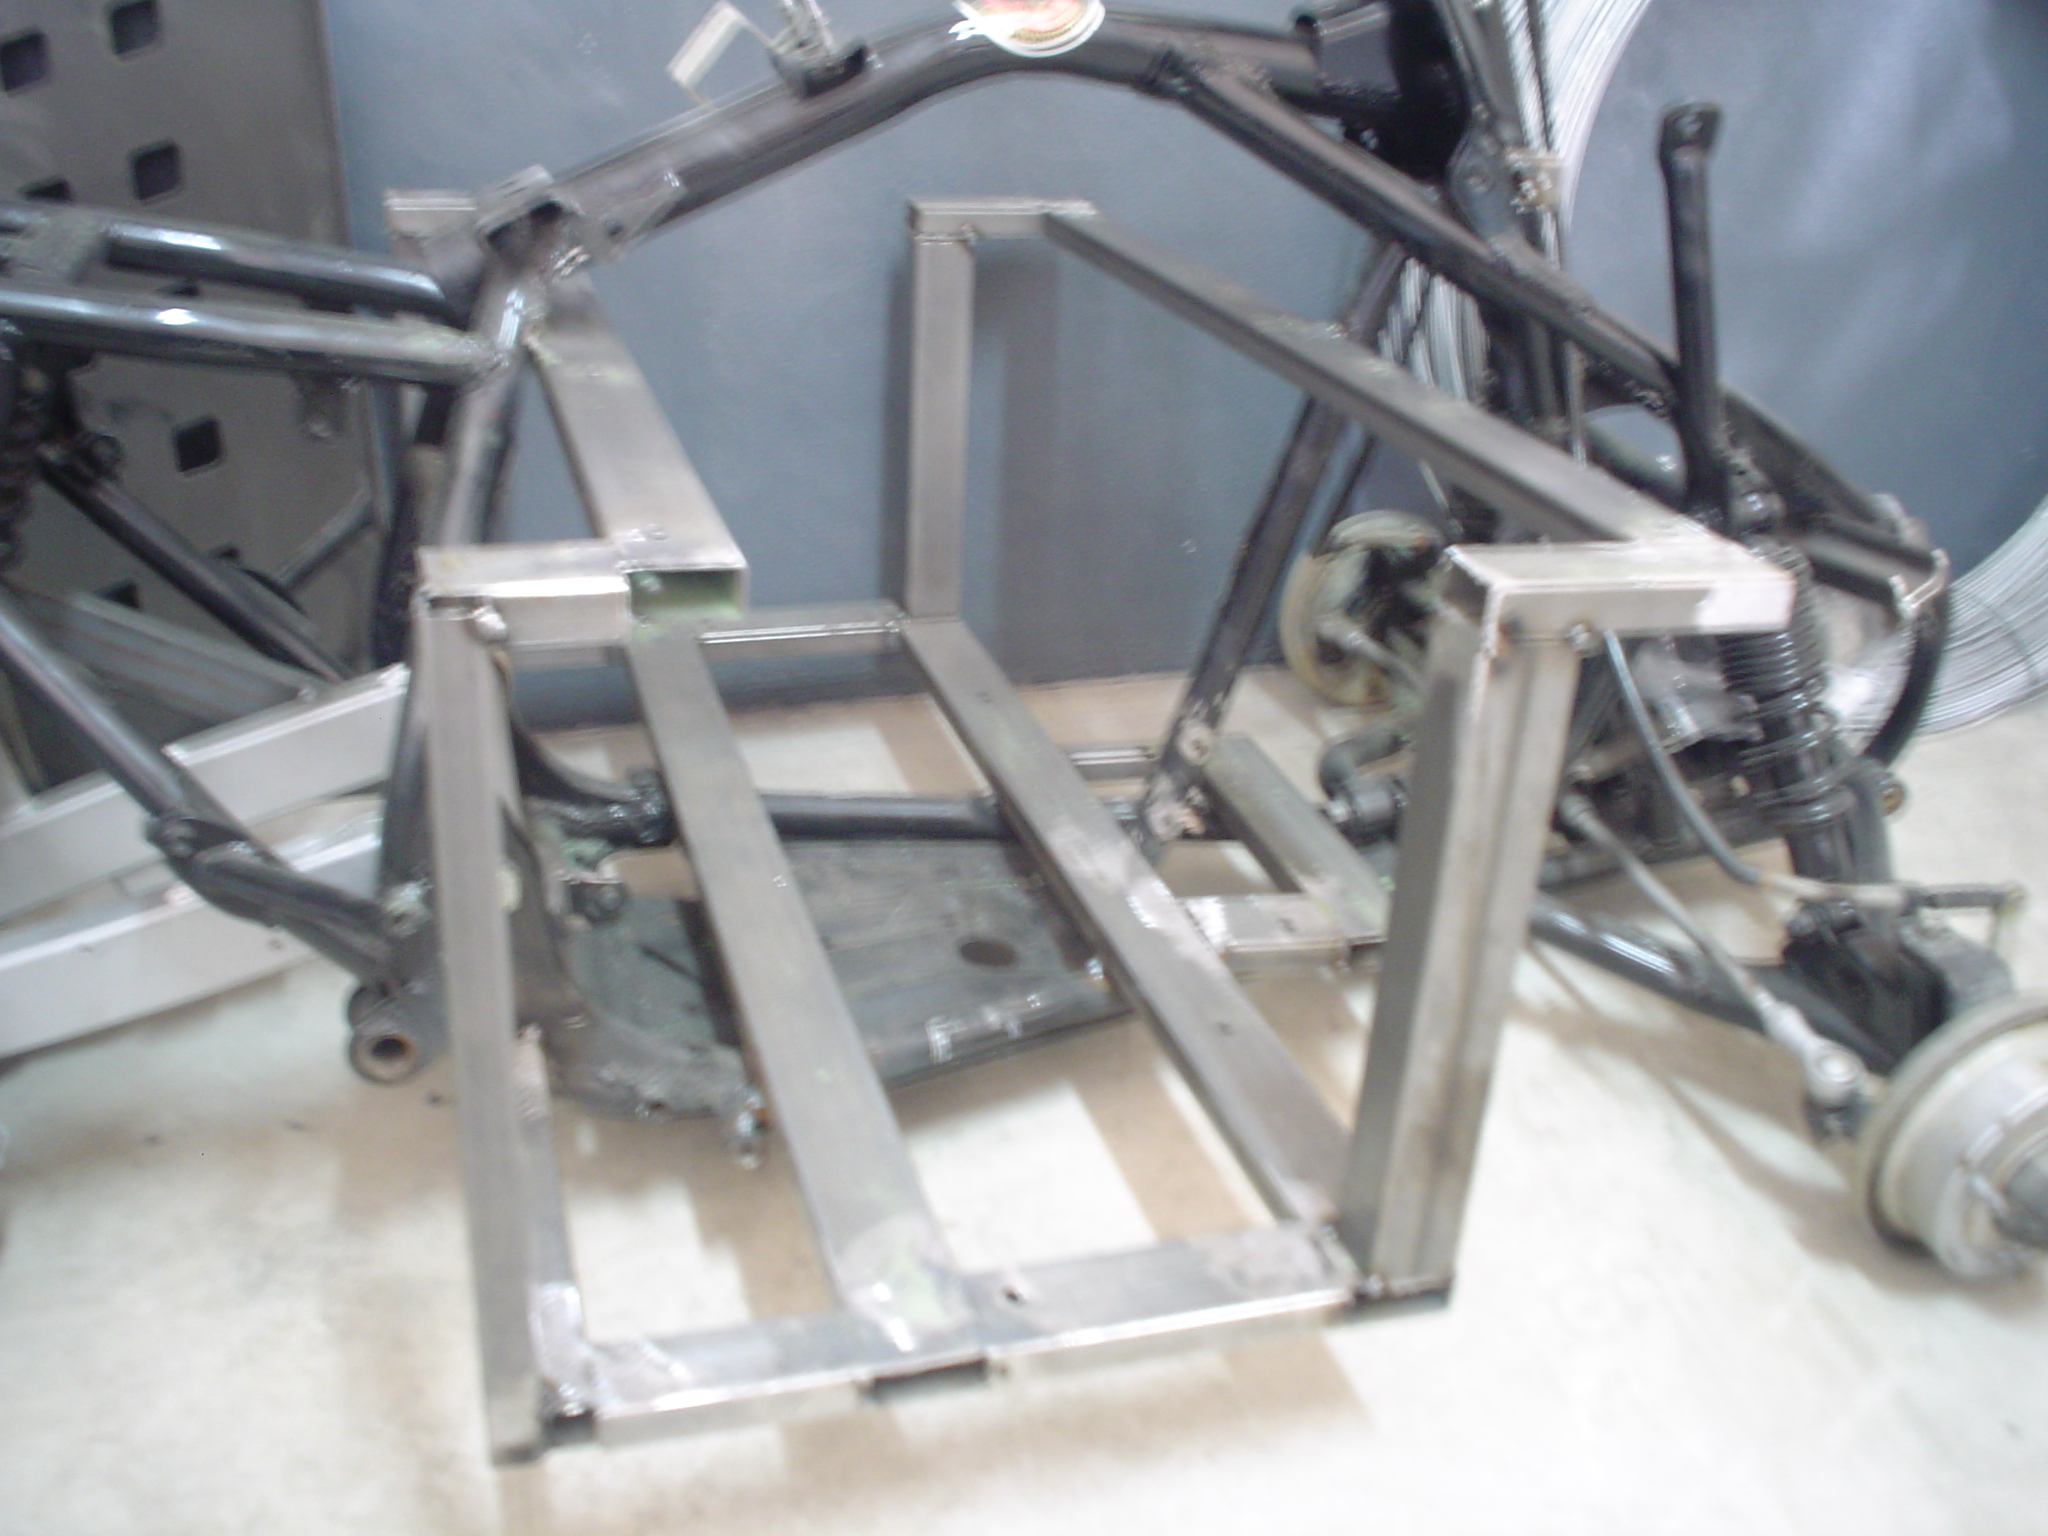
\includegraphics[width=\linewidth]{recursos/imagens/apendicef/chassi_estrutura_plataformas}}
\end{subfigure}
\par\bigskip
\begin{subfigure}[b]{.45\linewidth}
    \subcaptionbox{Plataformas de madeira cortadas � medida, vistas de cima. Note-se os furos escareados.\label{fig:chassi_plataformas_cima}}{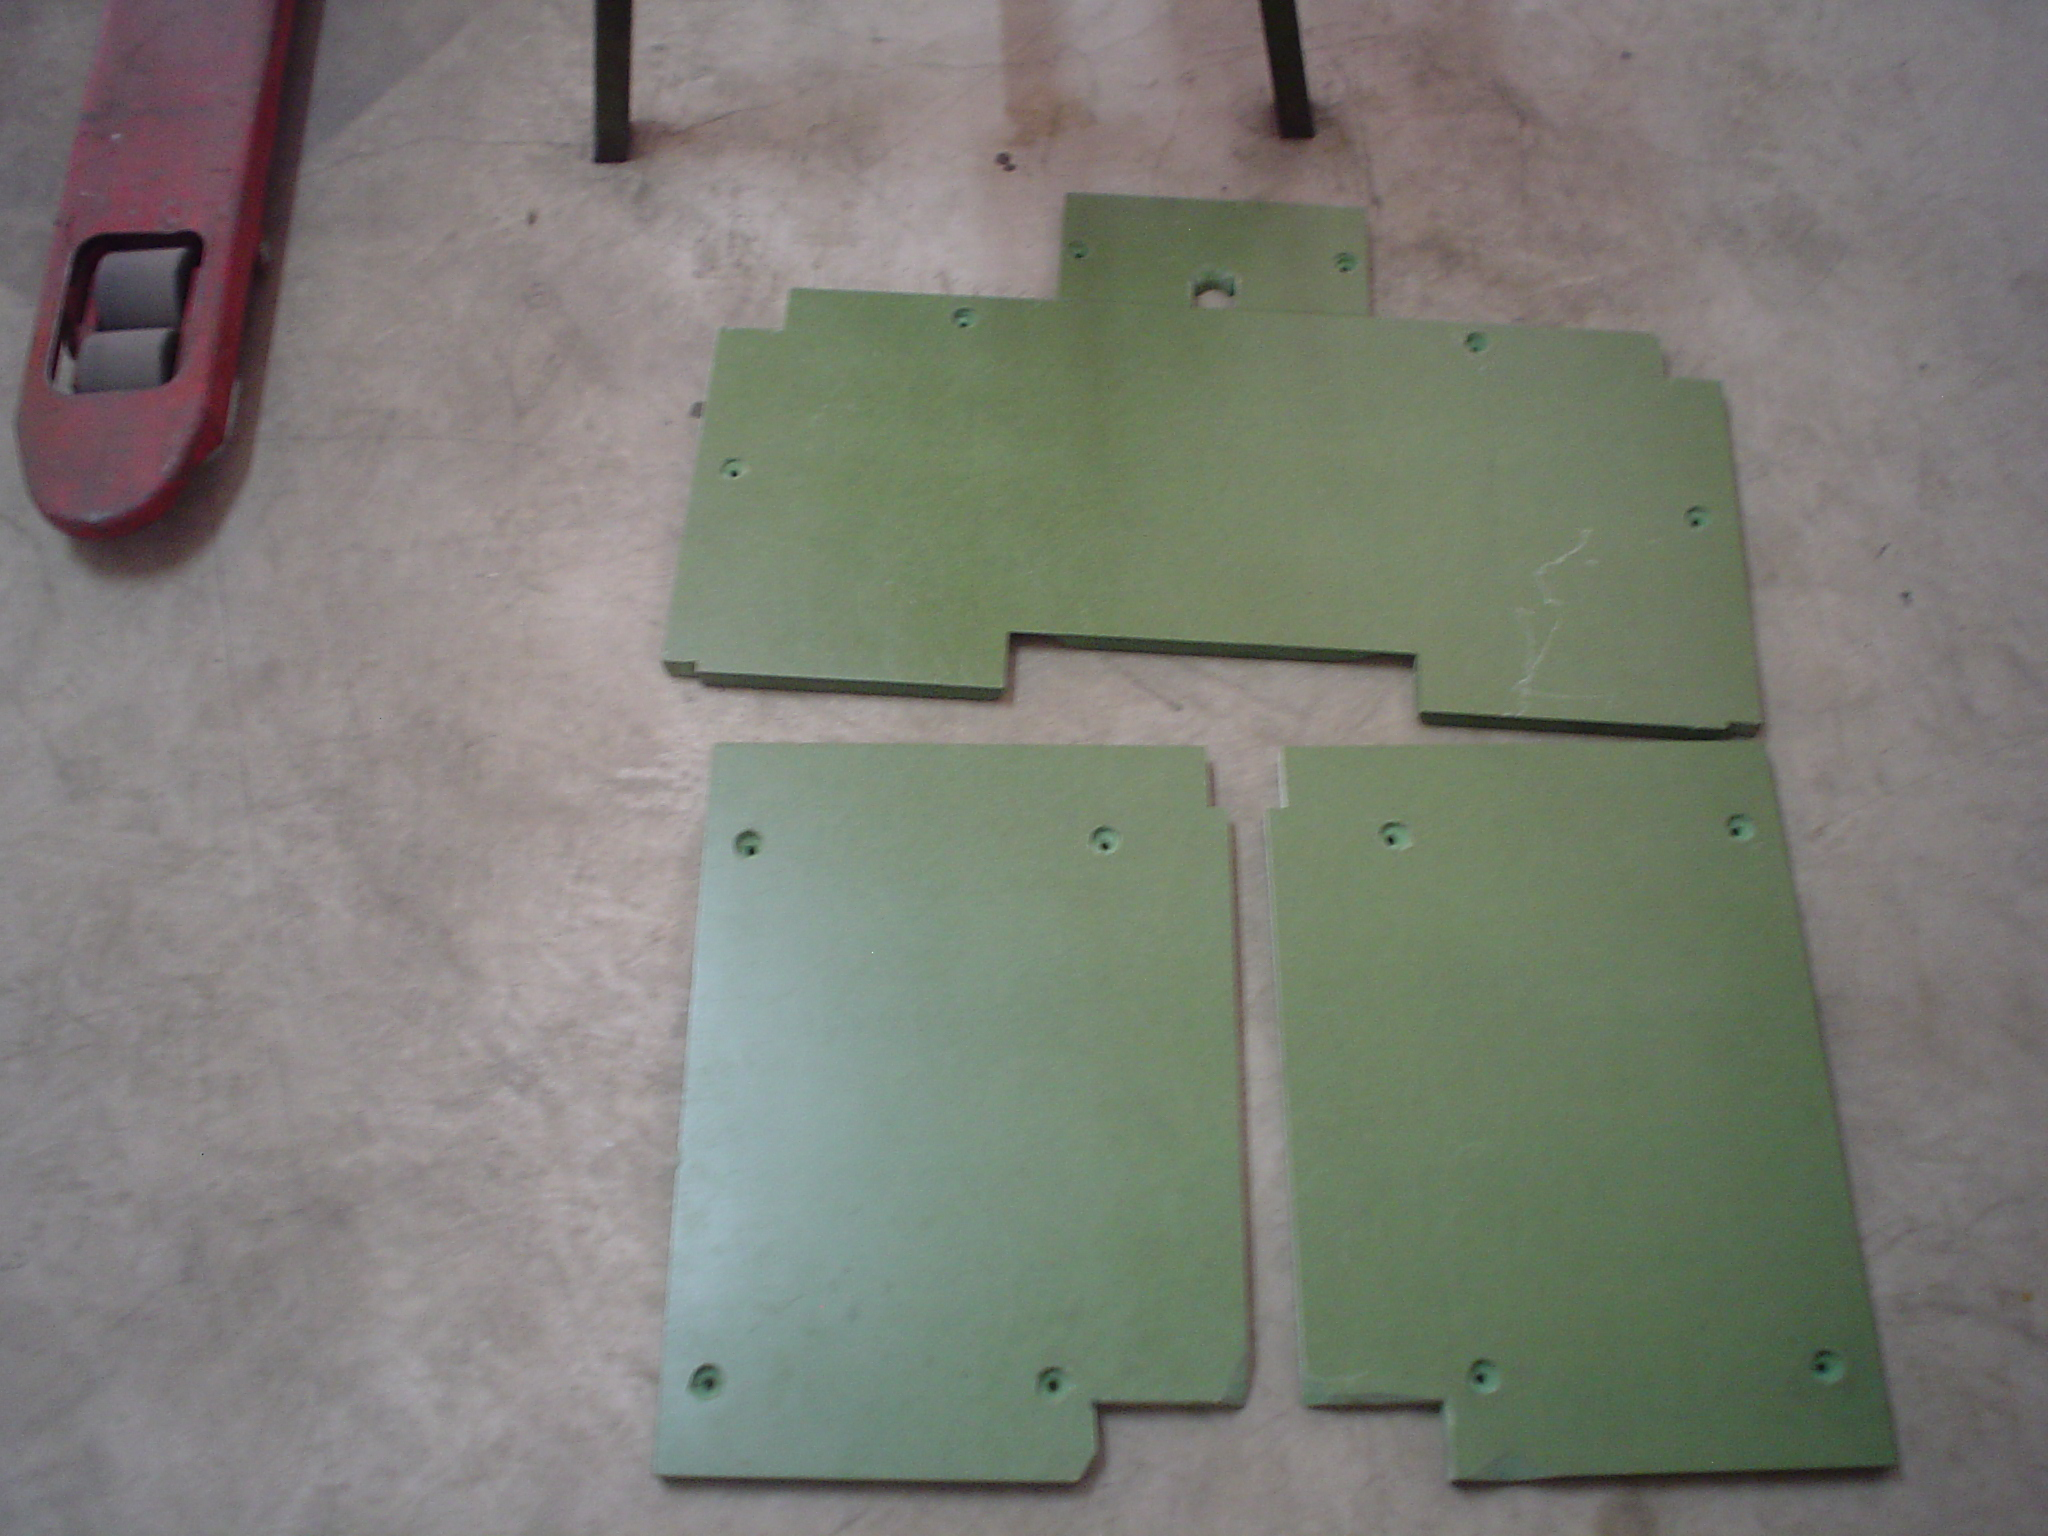
\includegraphics[width=\linewidth]{recursos/imagens/apendicef/chassi_madeira_plataformas} }
\end{subfigure}
\qquad
\begin{subfigure}[b]{.45\linewidth}
    \subcaptionbox{Plataformas inferior e superior de bombordo assentes na estrutura.\label{fig:chassi_plataformas}}{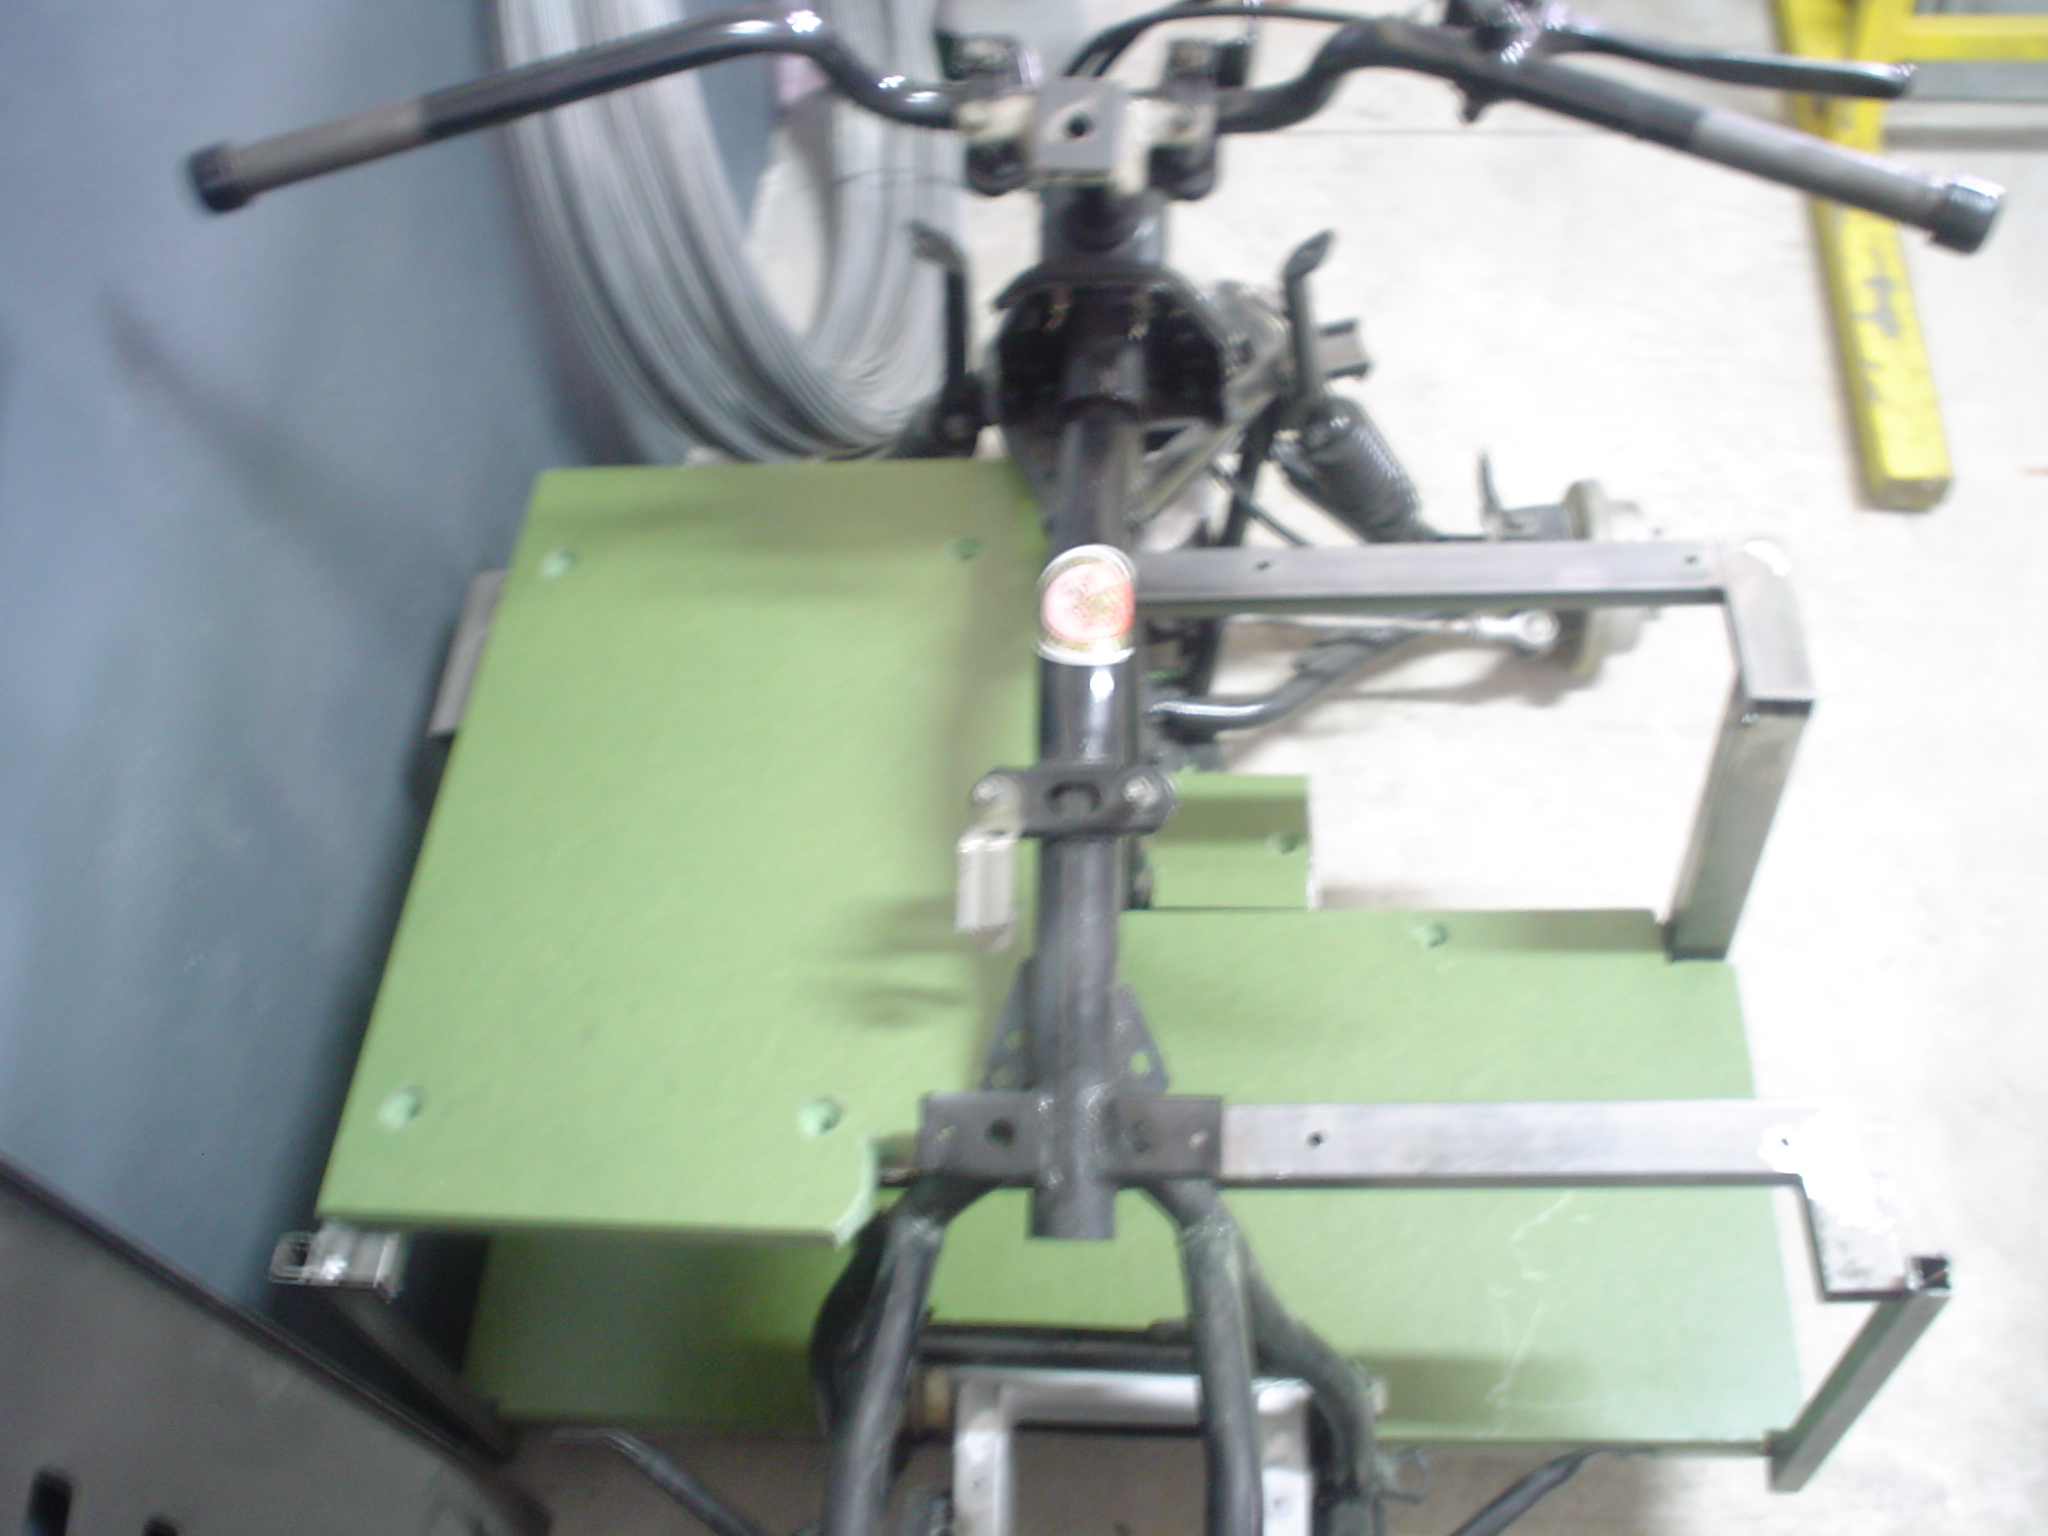
\includegraphics[width=\linewidth]{recursos/imagens/apendicef/chassi_plataformas} }
\end{subfigure}
\par\bigskip
\begin{subfigure}[b]{.45\linewidth}
    \subcaptionbox{Plataforma inferior (das baterias) com os batentes colados. Note-se que os parafusos de fixa��o ficam abaixo do n�vel da plataforma.\label{fig:chassi_plataforma_inferior}}{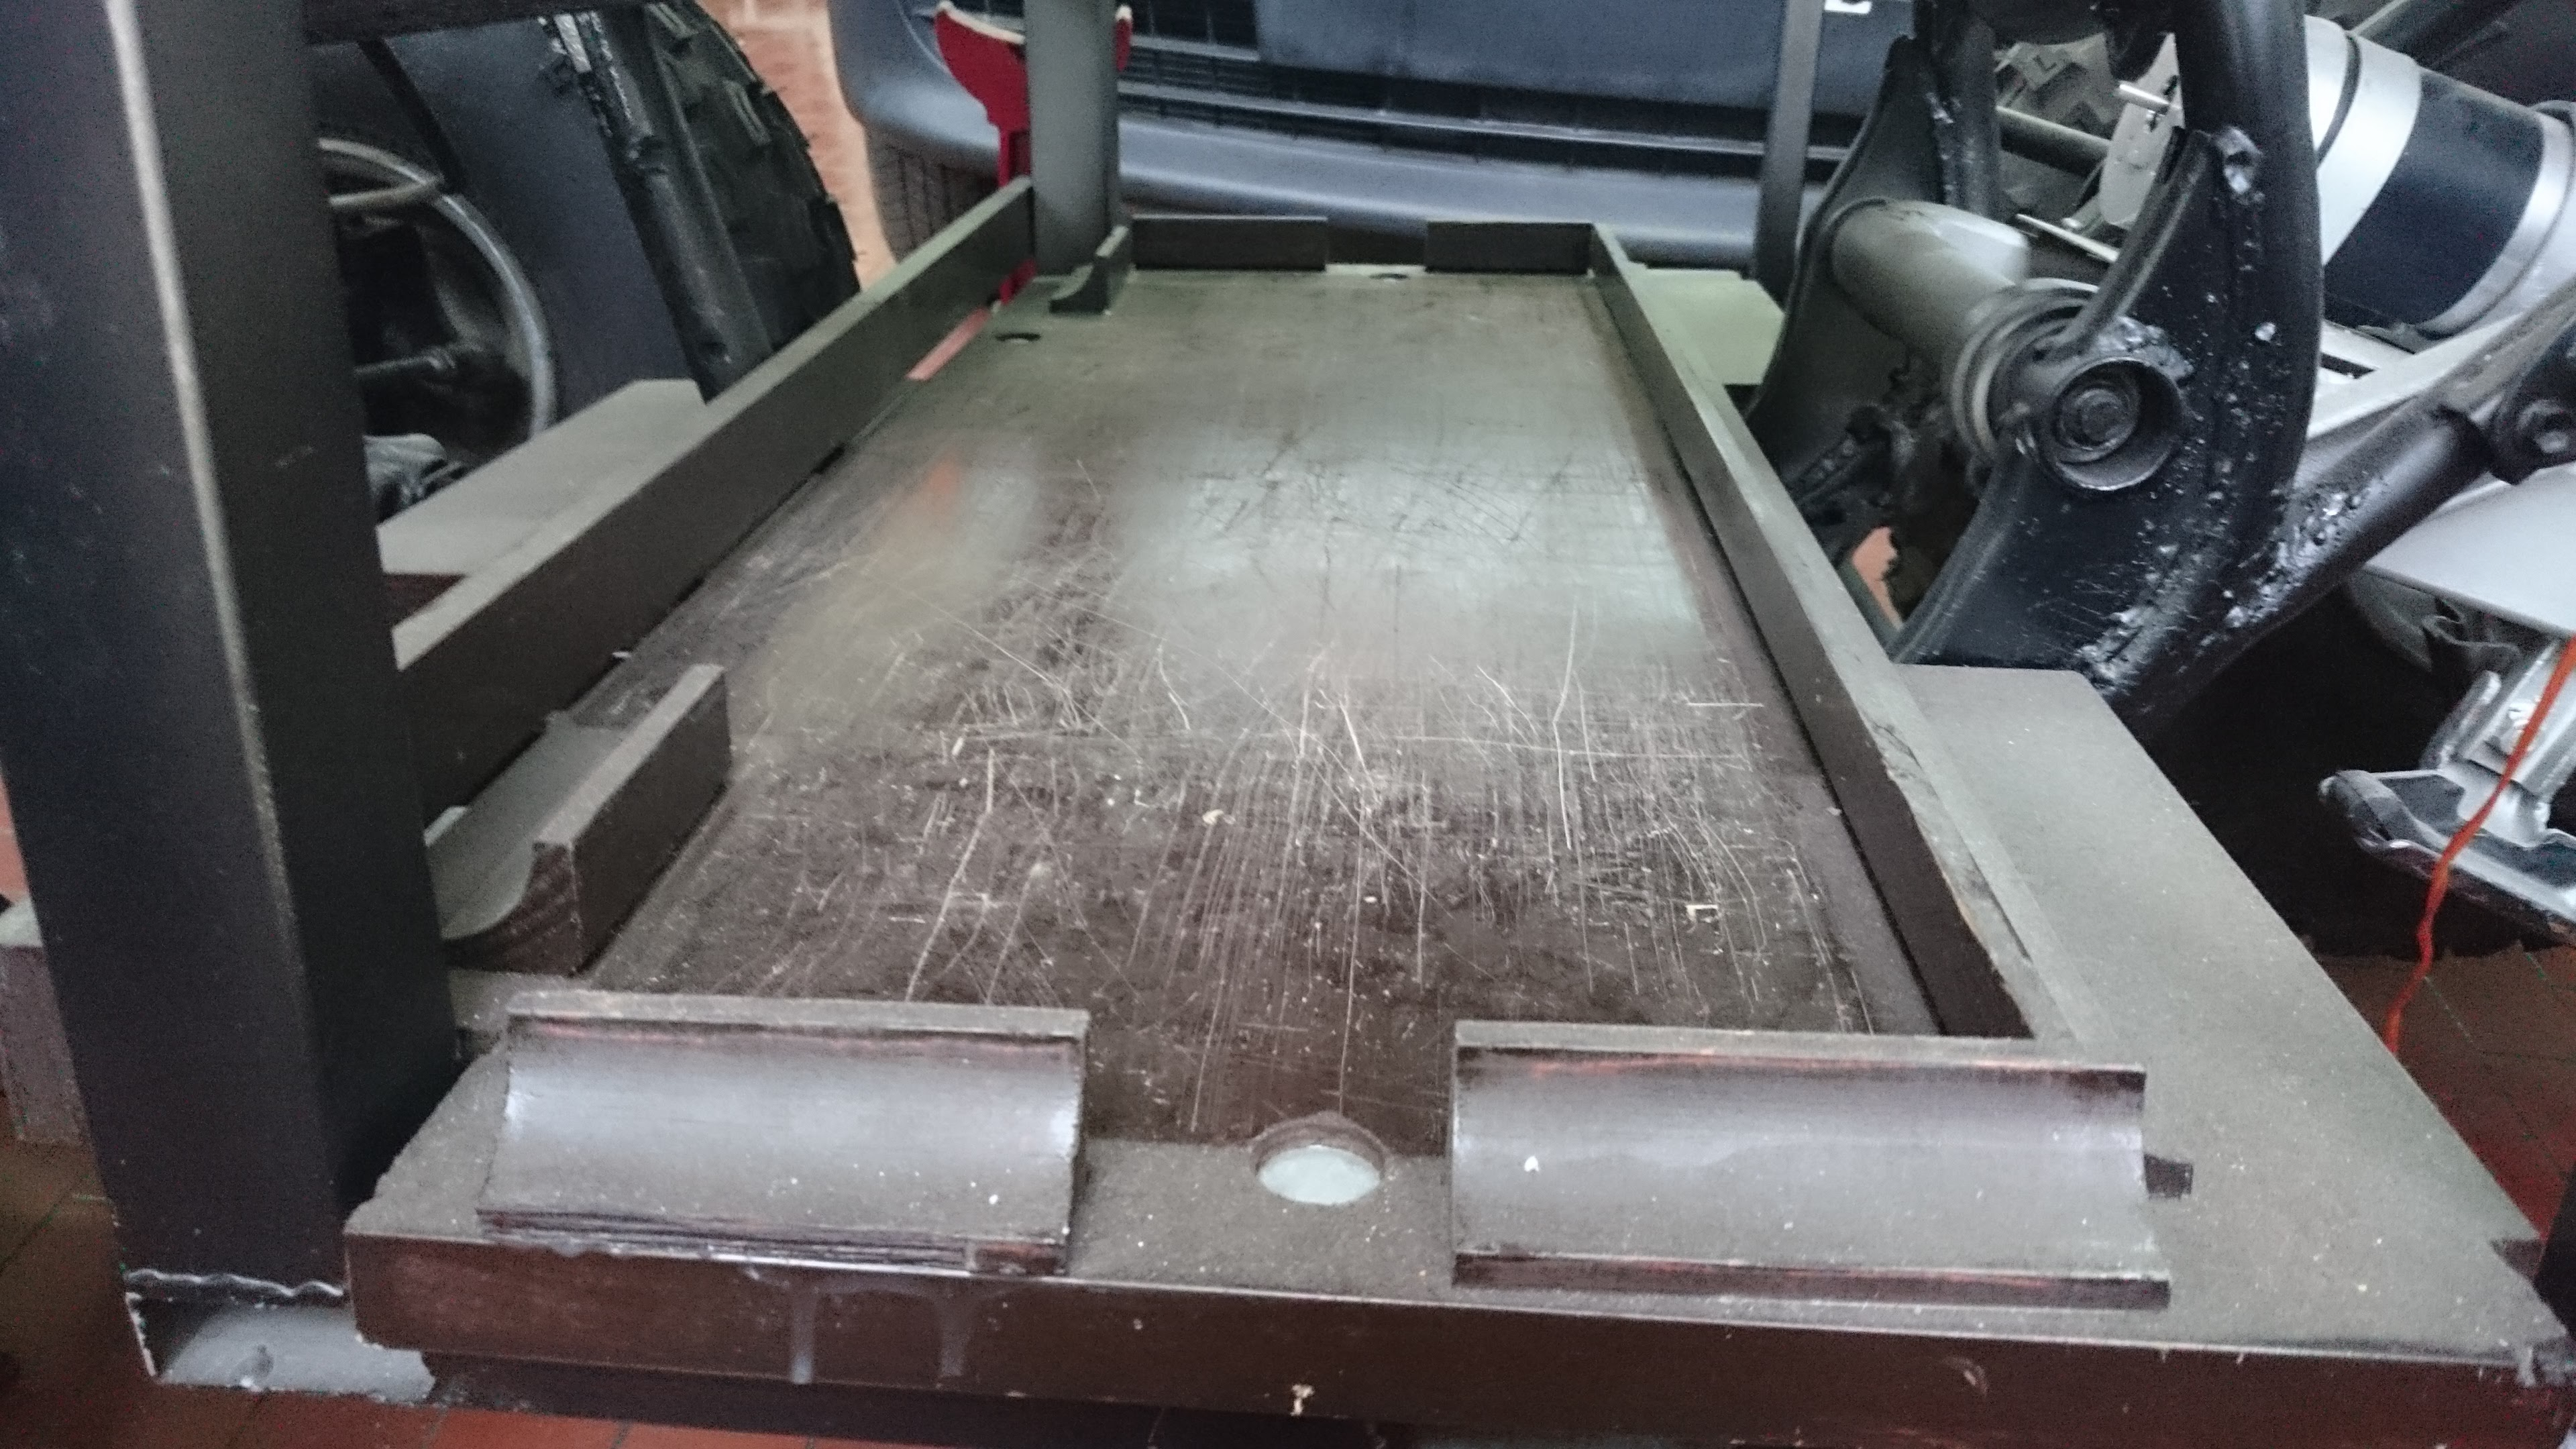
\includegraphics[width=\linewidth]{recursos/imagens/apendicef/chassi_plataforma_inferior} }
\end{subfigure}
\qquad
\begin{subfigure}[b]{.45\linewidth}
    \subcaptionbox{Conjunto das baterias � carga, fora do ve�culo. Note-se o carregador dedicado, � direita.\label{fig:baterias_carga}}{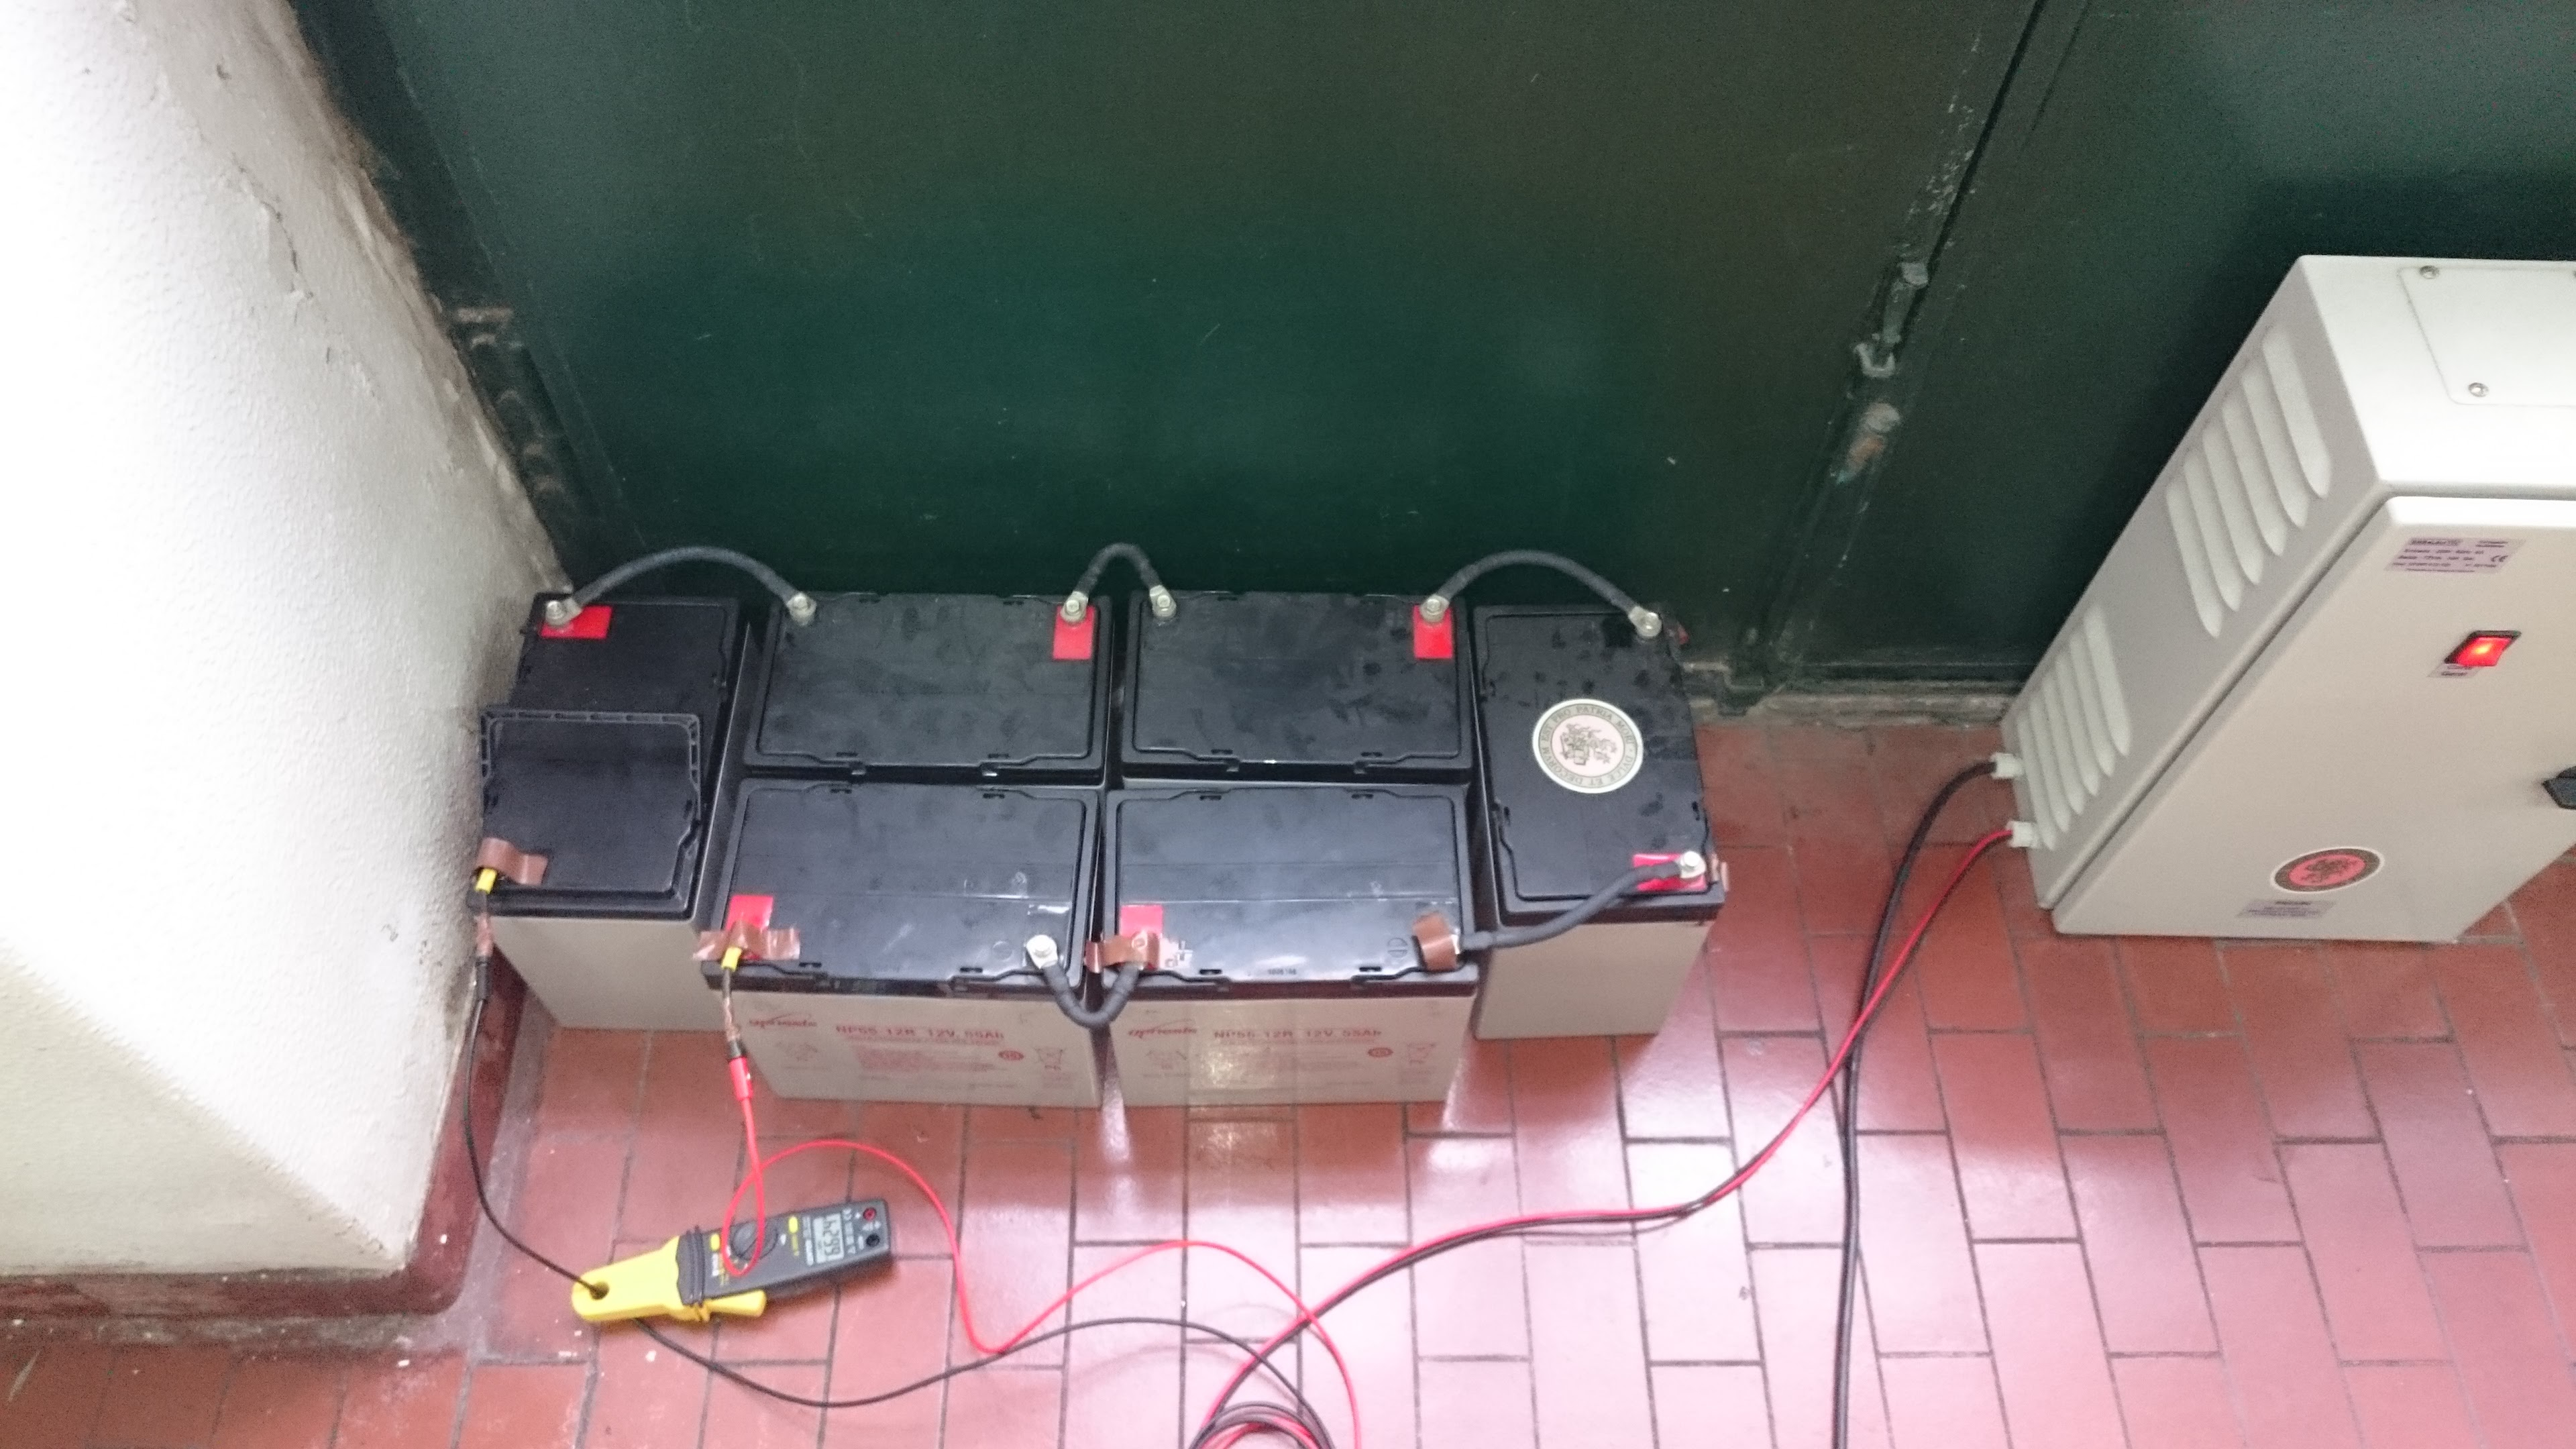
\includegraphics[width=\linewidth]{recursos/imagens/apendicef/bateria_carregando} }
\end{subfigure}
\end{figure}
%next page
\begin{figure}
\ContinuedFloat
\begin{subfigure}[b]{.45\linewidth}
    \subcaptionbox{Bateria danificada ap�s carga fora da vida �til. Note-se que apesar de ter "inchado", a bateria n�o explodiu.\label{fig:baterias_inchada}}{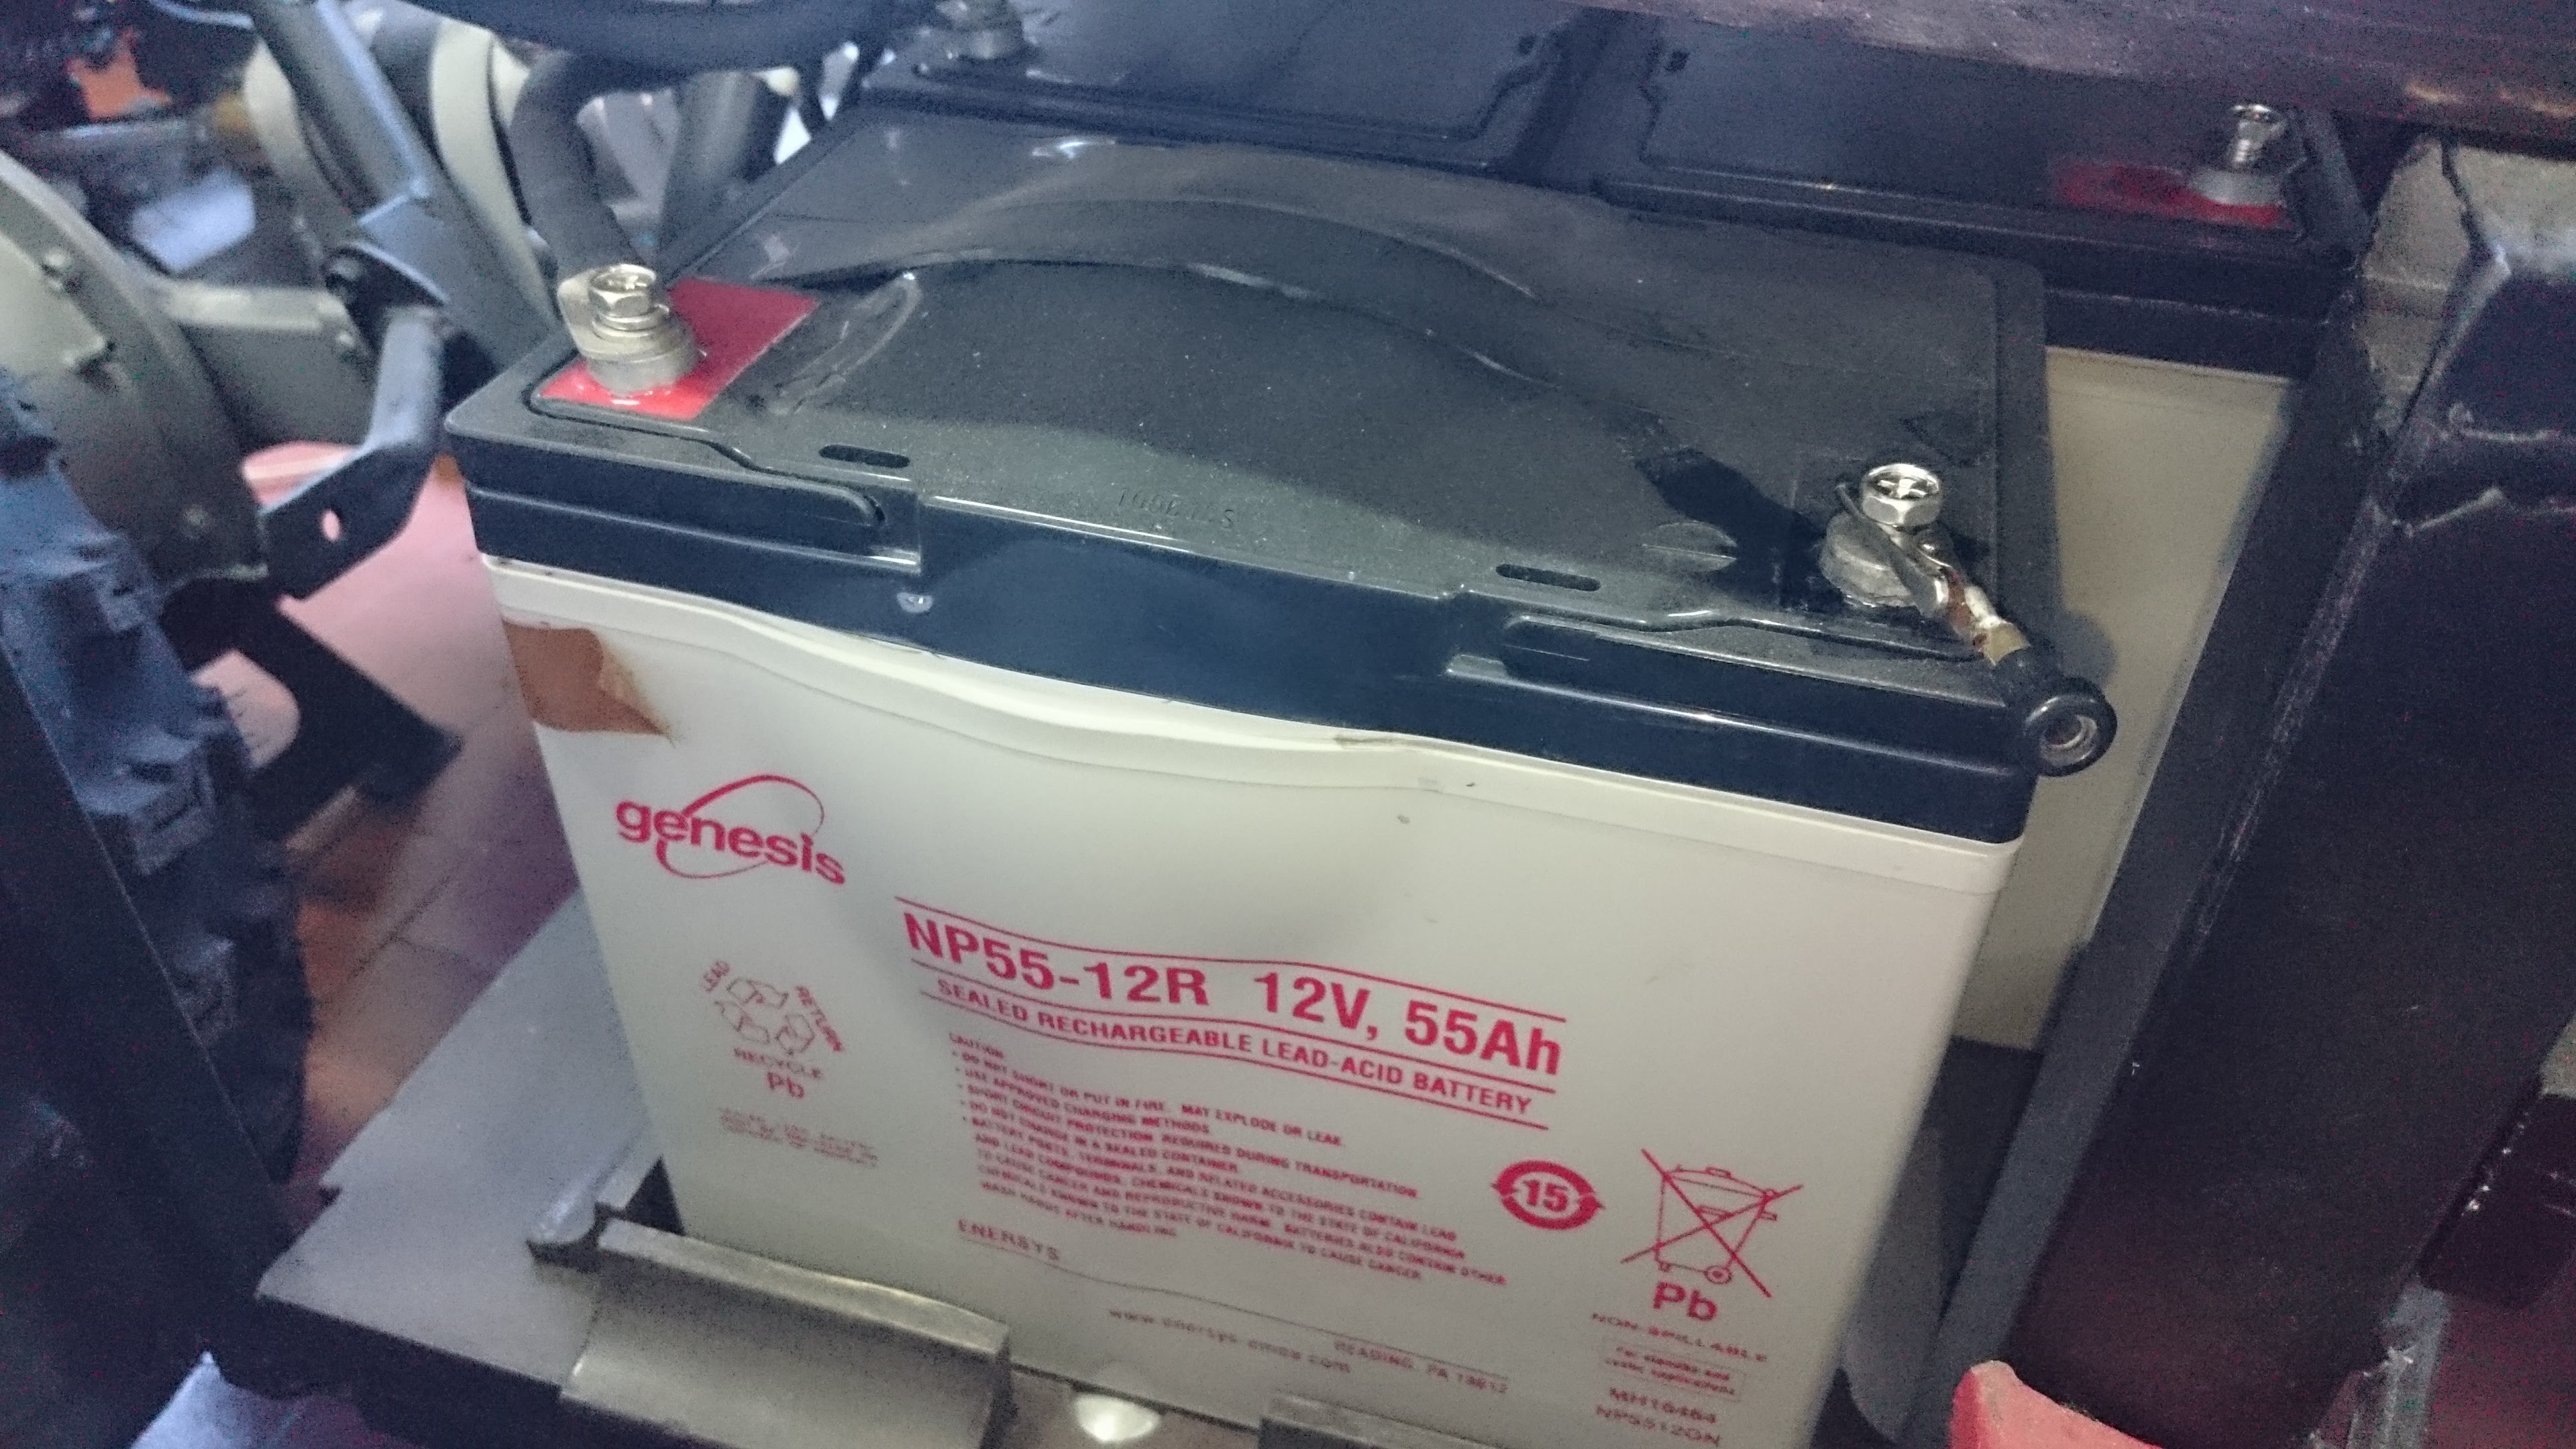
\includegraphics[width=\linewidth]{recursos/imagens/apendicef/bateria_inchada} }
\end{subfigure}
\qquad
\begin{subfigure}[b]{.45\linewidth}
    \subcaptionbox{Plataforma do motor do trav�o. Note-se o espa�o entre a plataforma e a forquilha traseira, ocupado por anilhas de borracha.\label{fig:trv_plataforma}}{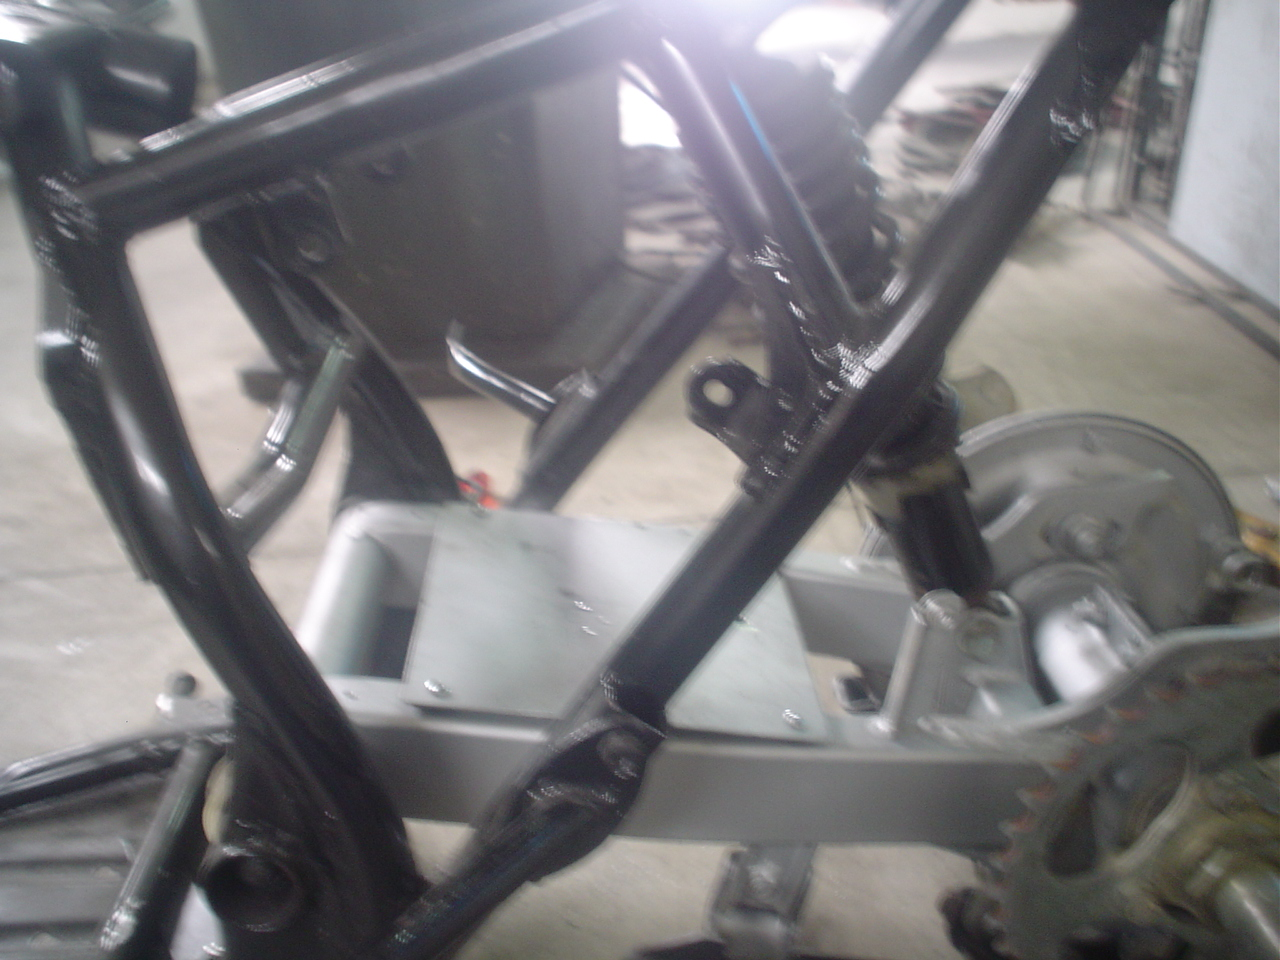
\includegraphics[width=\linewidth]{recursos/imagens/apendicef/trv_plataforma} }
\end{subfigure}
\par\bigskip
\begin{subfigure}[b]{.45\linewidth}
    \subcaptionbox{Pormenor do tambor do trav�o e da alavanca de acionamento.\label{fig:trv_alavanca}}{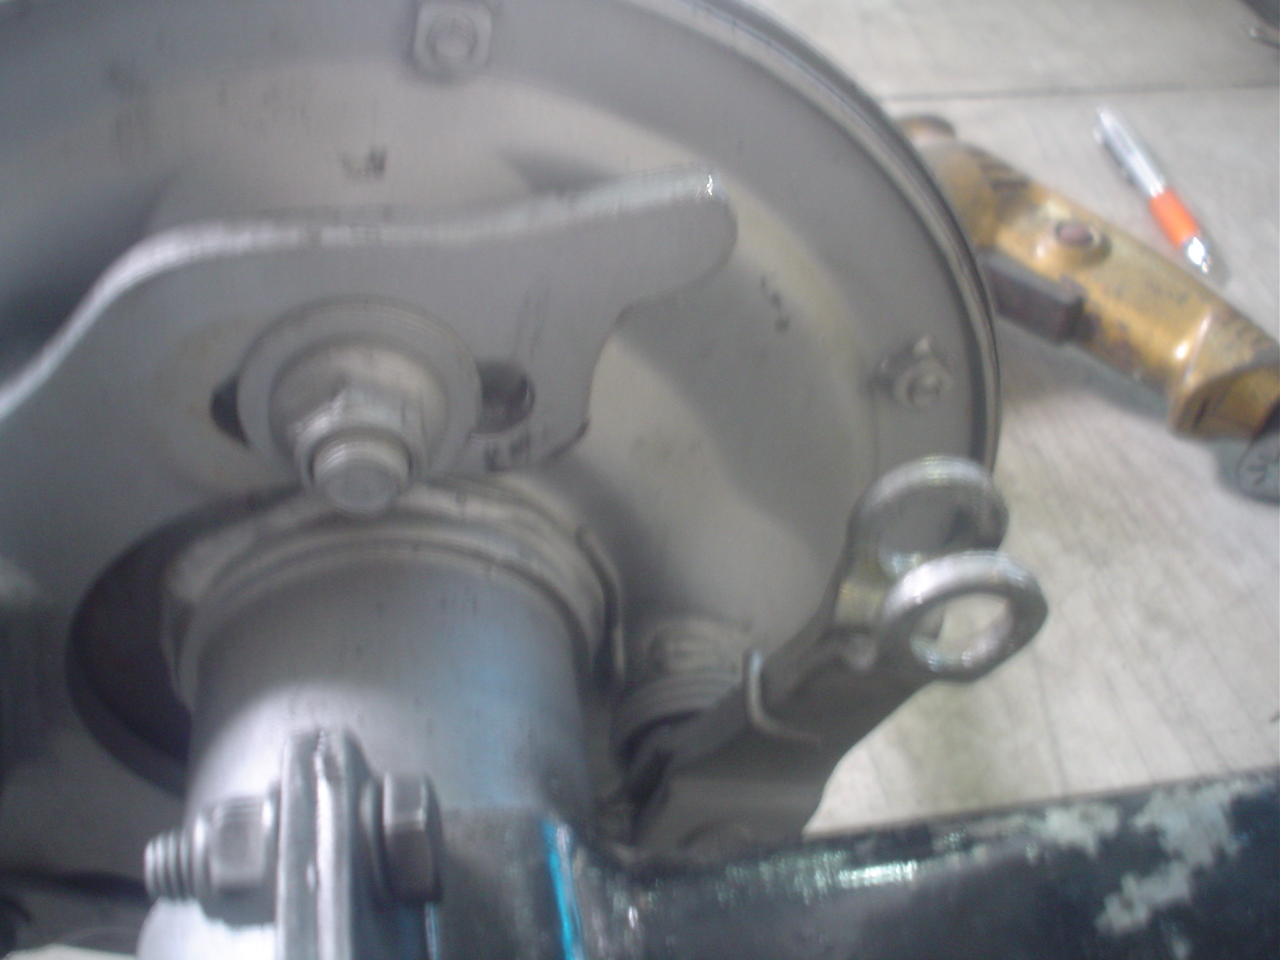
\includegraphics[width=\linewidth]{recursos/imagens/apendicef/trv_alavanca} }
\end{subfigure}
\qquad
\begin{subfigure}[b]{.45\linewidth}
    \subcaptionbox{Montagem de fixa��o da alavanca do trav�o ao piv�. Apesar de n�o ser vis�vel na imagem, as duas barras de ferro paralelas est�o furadas em ambas as pontas.\label{fig:trv_fixador_alavanca}}{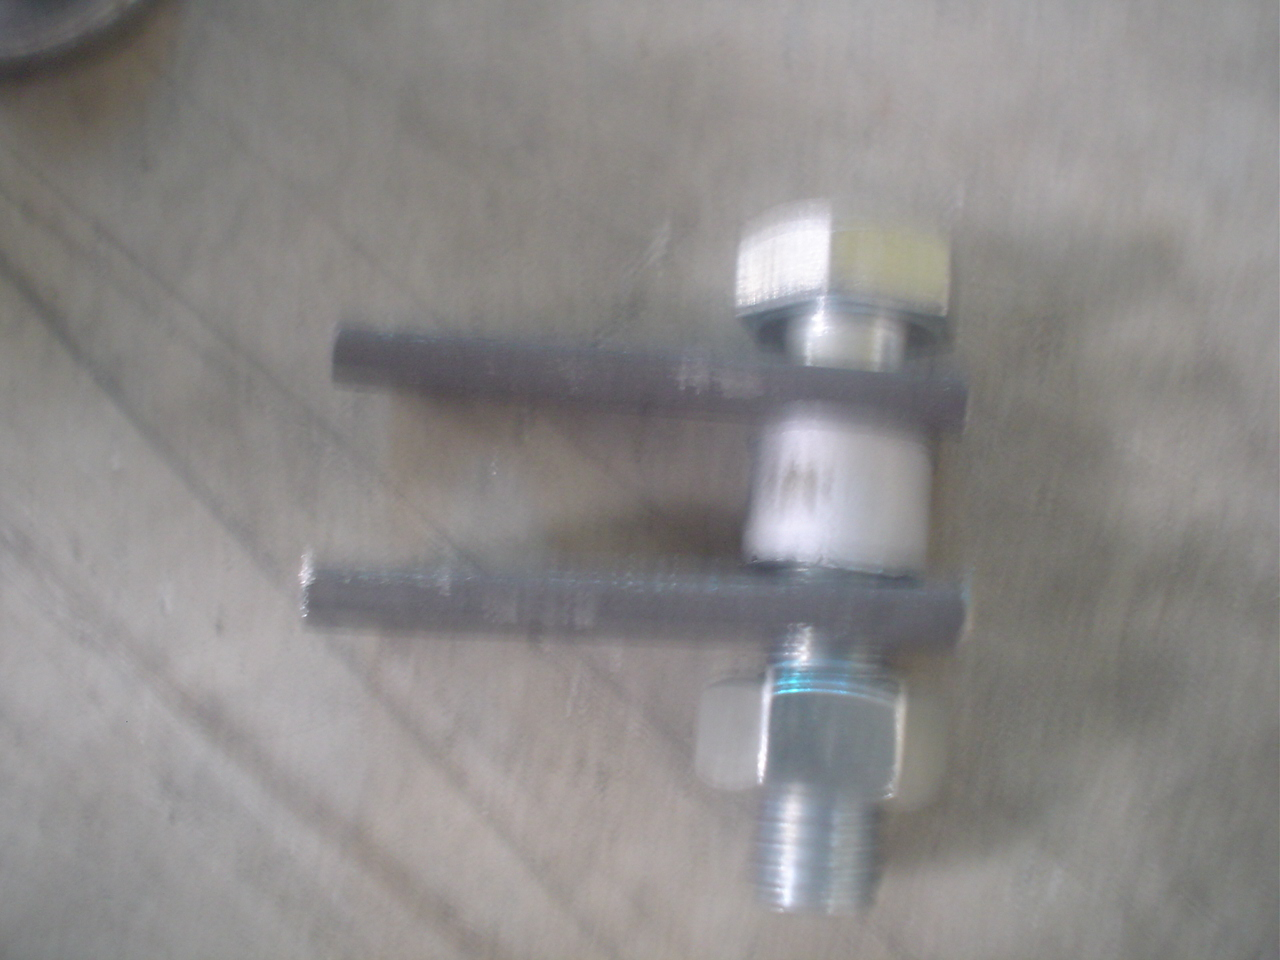
\includegraphics[width=\linewidth]{recursos/imagens/apendicef/trv_fixador_alavanca} }
\end{subfigure}
\par\bigskip
\begin{subfigure}[b]{.45\linewidth}
    \subcaptionbox{Piv� do trav�o traseiro. As sali�ncias cil�ndricas encaixam no fixador da alavanca, e o furo no topo � a rosca onde entra o parafuso sem fim.\label{fig:trv_pivo}}{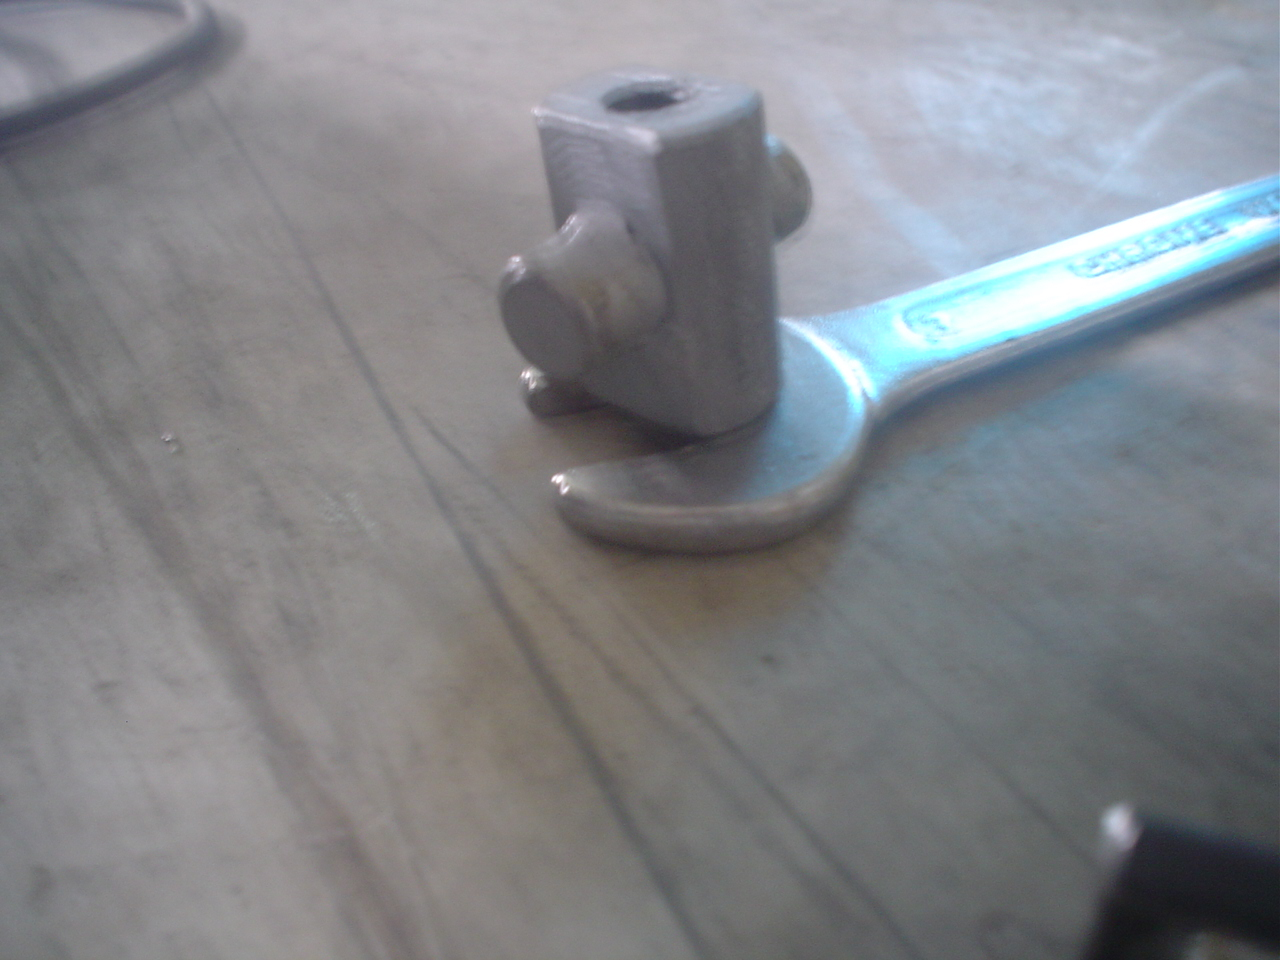
\includegraphics[width=\linewidth]{recursos/imagens/apendicef/trv_pivo} }
\end{subfigure}
\qquad
\begin{subfigure}[b]{.45\linewidth}
    \subcaptionbox{Adaptador de lat�o instalado no veio do motor do trav�o, e bra�adeira frontal de fixa��o do motor.\label{fig:trv_adaptador_bracadeira}}{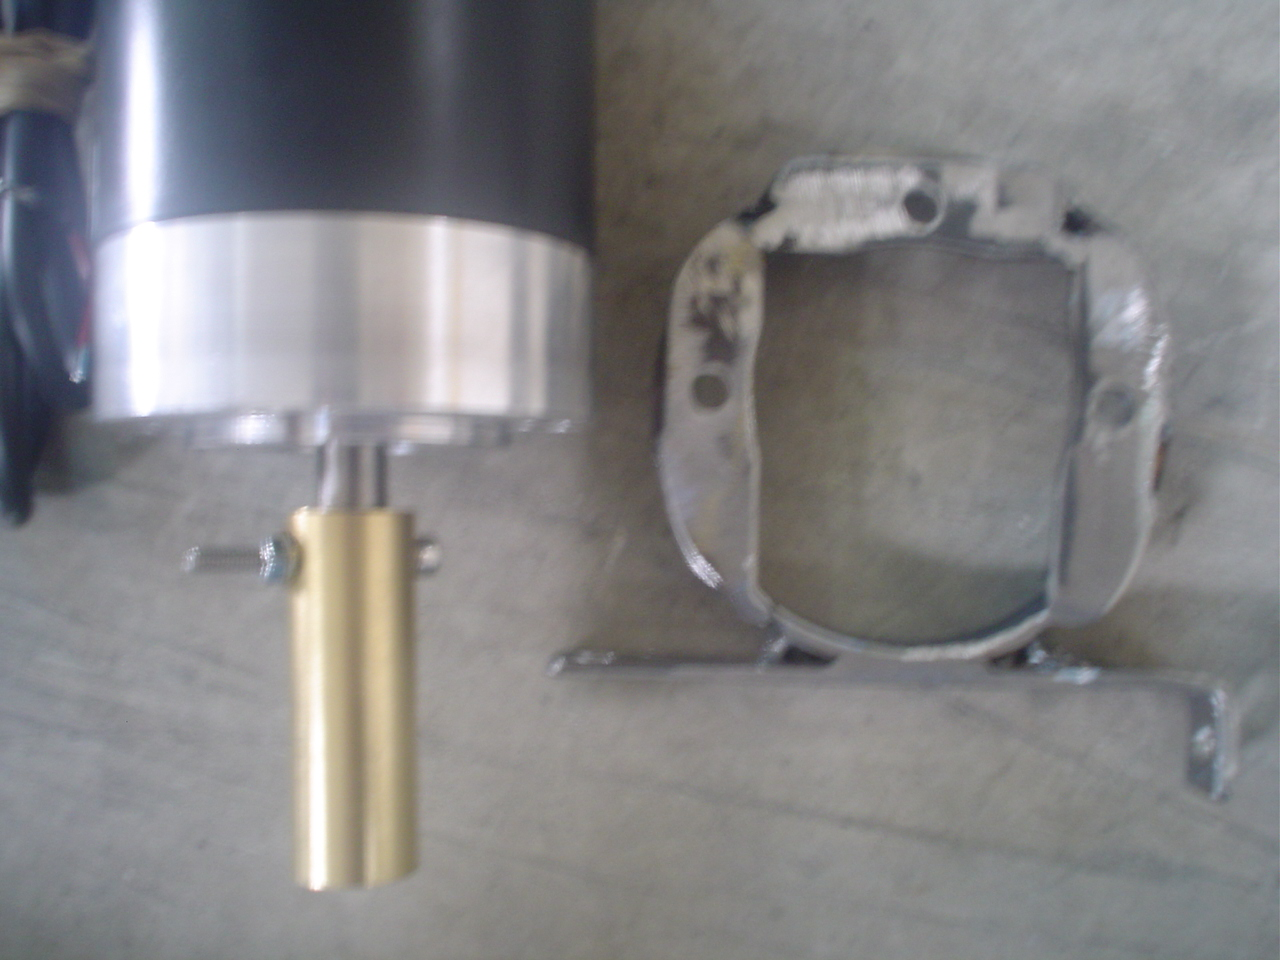
\includegraphics[width=\linewidth]{recursos/imagens/apendicef/trv_adaptador_bracadeira} }
\end{subfigure}
\end{figure}
%next page
\begin{figure}
\ContinuedFloat
\begin{subfigure}[b]{.45\linewidth}
    \subcaptionbox{Motor do trav�o instalado no ve�culo, visto de lado. Note-se as duas bra�adeiras de fixa��o do motor, e a porca e anilha de mola de fixa��o do parafuso sem fim ao adaptador.\label{fig:trv_motor_perfil}}{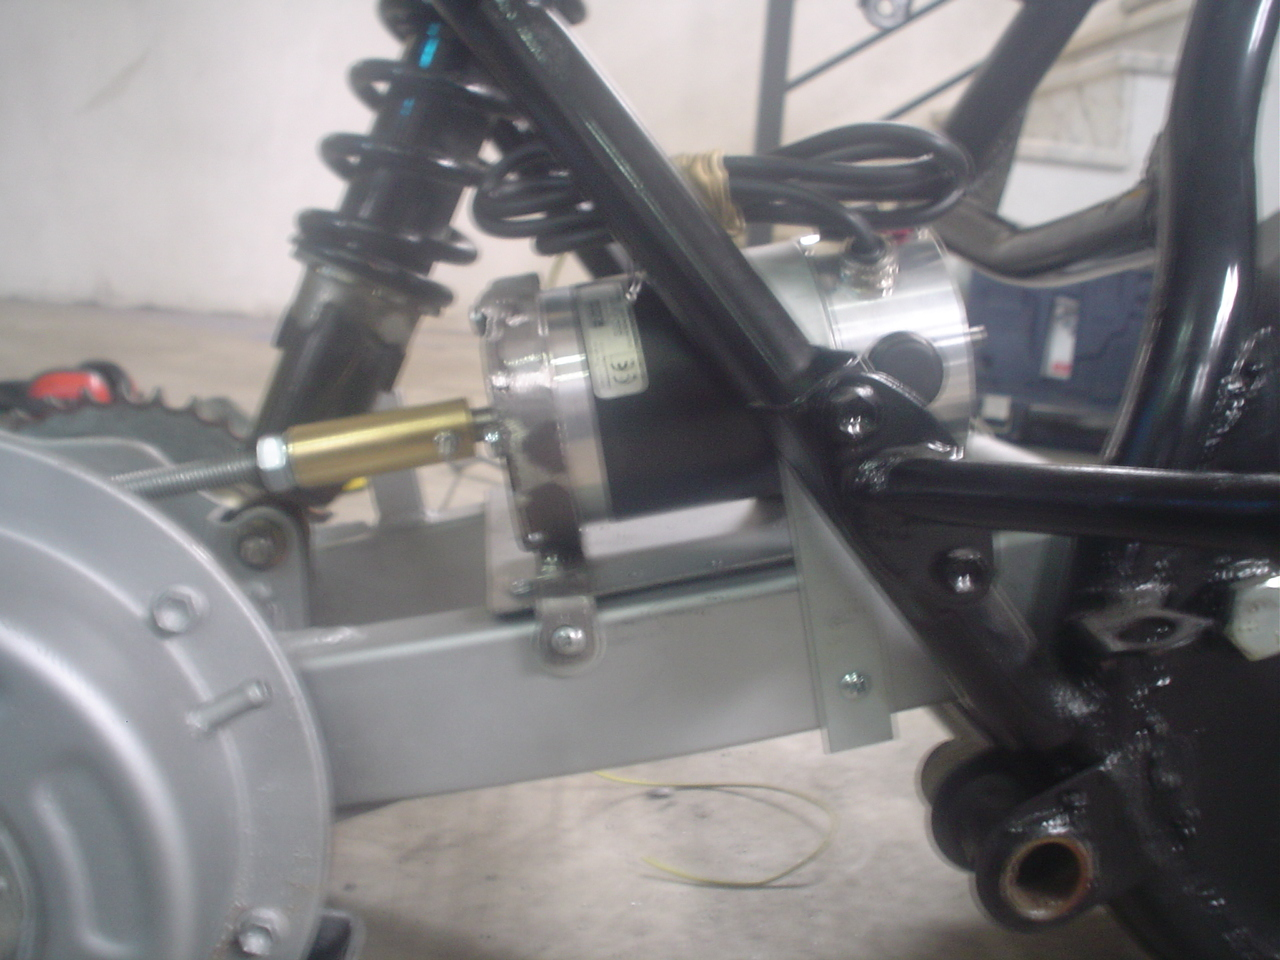
\includegraphics[width=\linewidth]{recursos/imagens/apendicef/trv_motor_perfil} }
\end{subfigure}
\qquad
\begin{subfigure}[b]{.45\linewidth}
    \subcaptionbox{Redutor da dire��o instalado na estrutura de suporte. A proje��o inicial saiu errada e a plataforma teve que ser alterada. Note-se tamb�m no cimo da imagem o suporte do esticador.\label{fig:dir_redutor_instalado}}{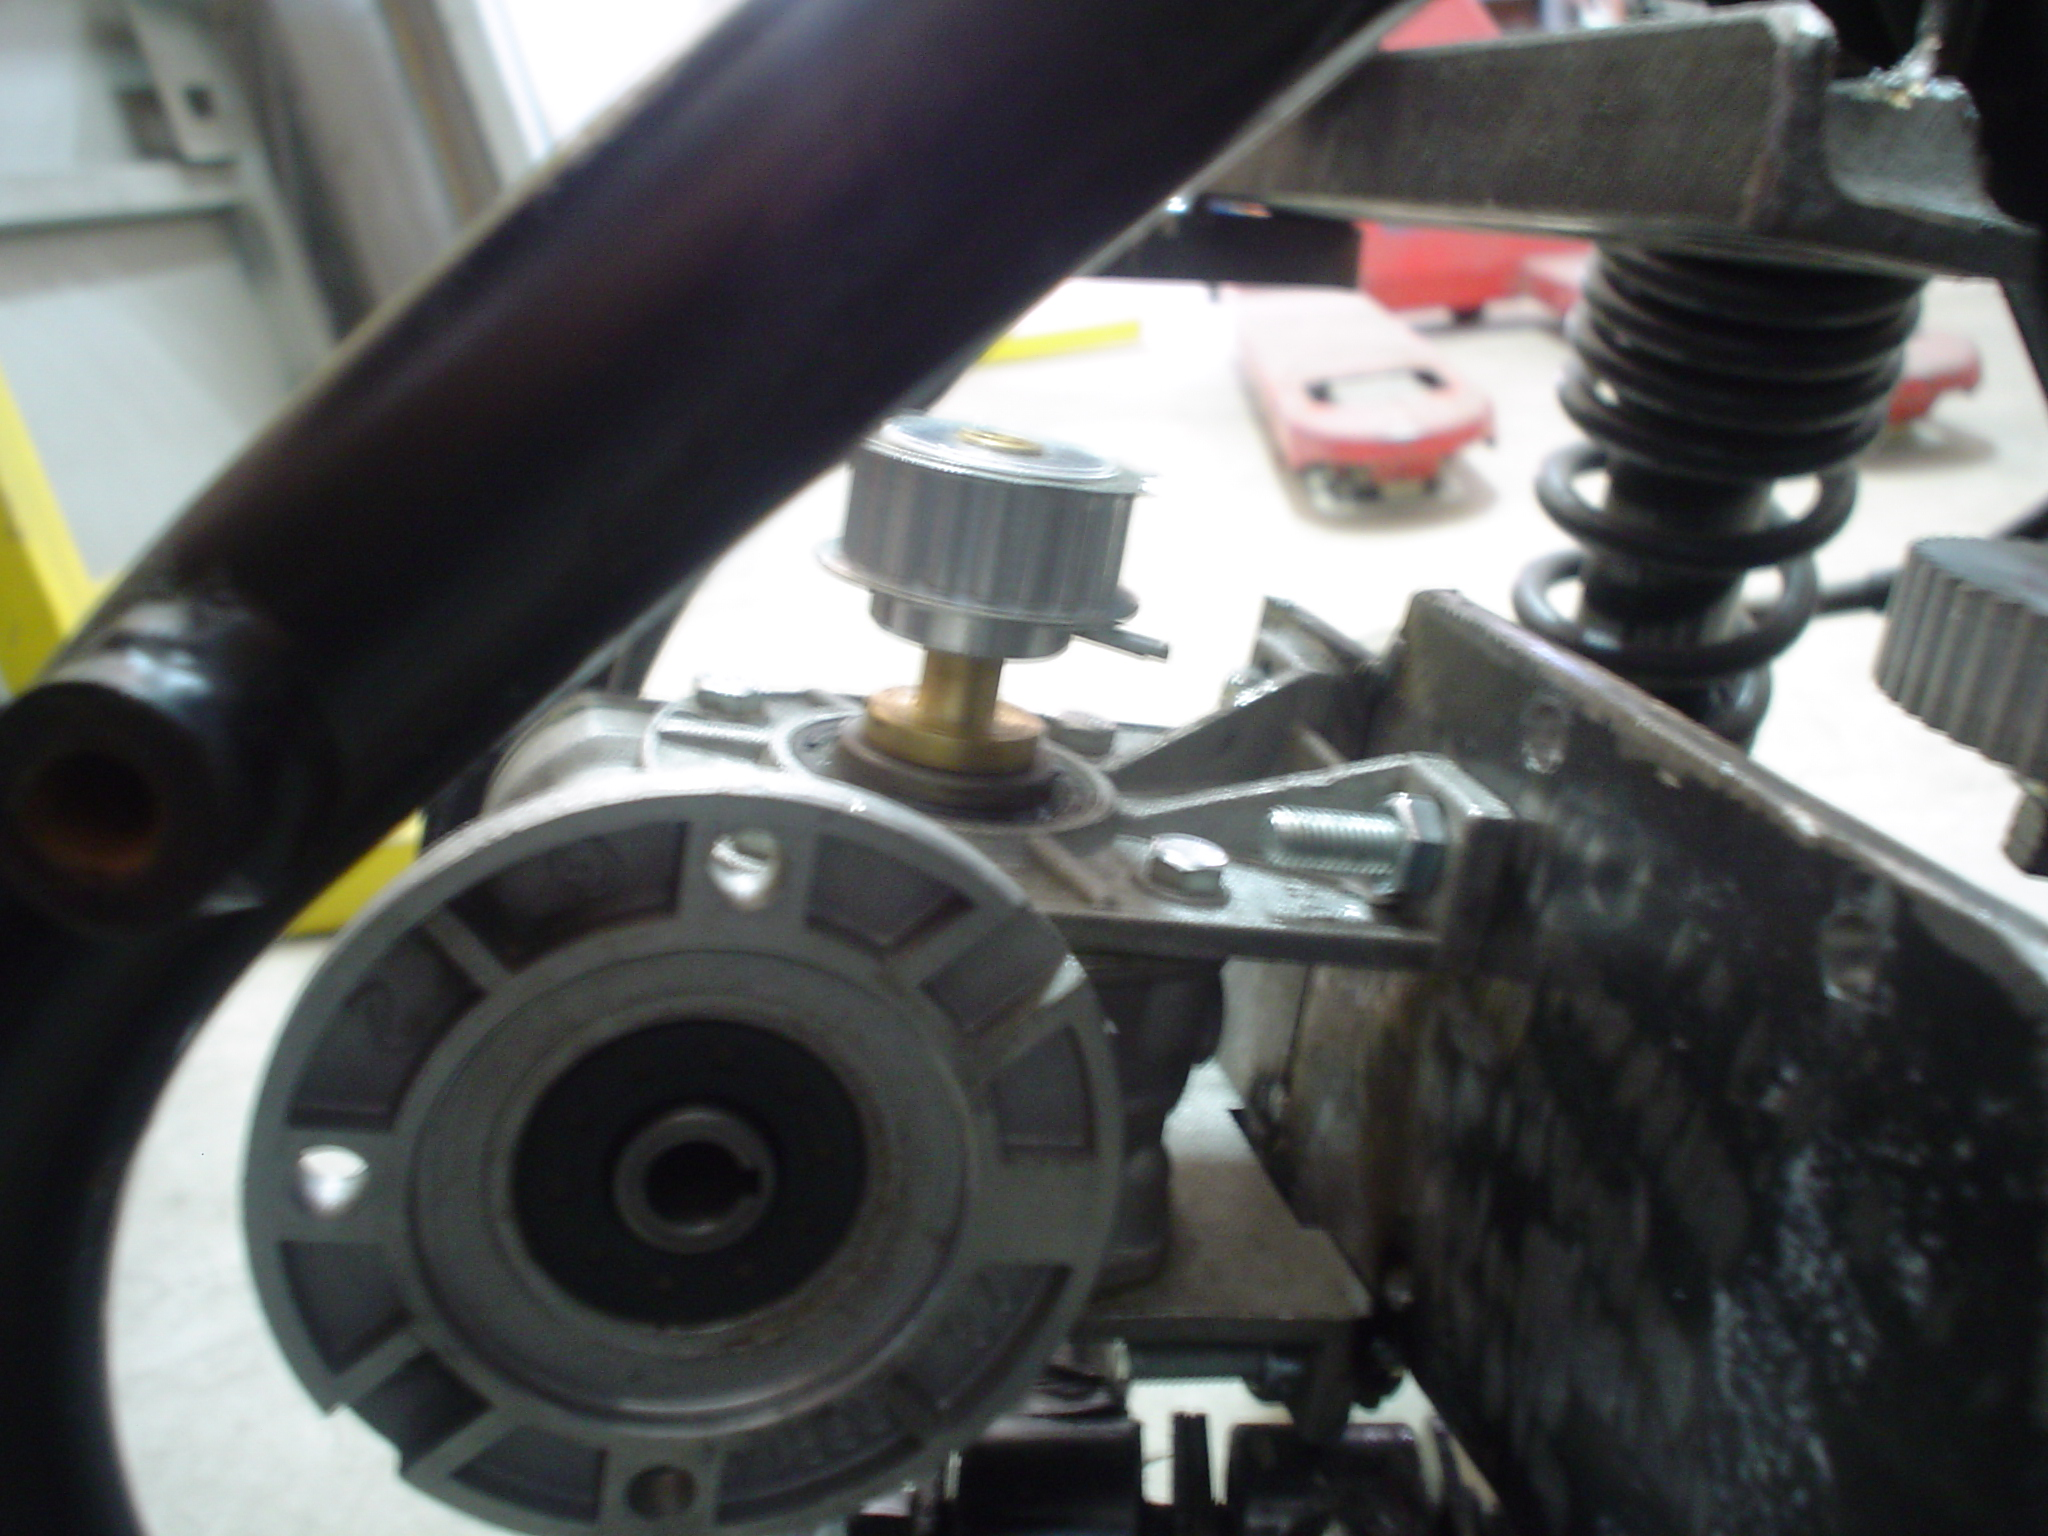
\includegraphics[width=\linewidth]{recursos/imagens/apendicef/dir_redutor_instalado} }
\end{subfigure}
\par\bigskip
\begin{subfigure}[b]{.45\linewidth}
    \subcaptionbox{Veio do redutor da dire��o com polia instalada. O veio prende no redutor atrav�s dos bocados de chapa inseridos na ranhura longitudinal, e fica com recurso ao parafuso e chapa de batente.\label{fig:dir_veio_redutor}}{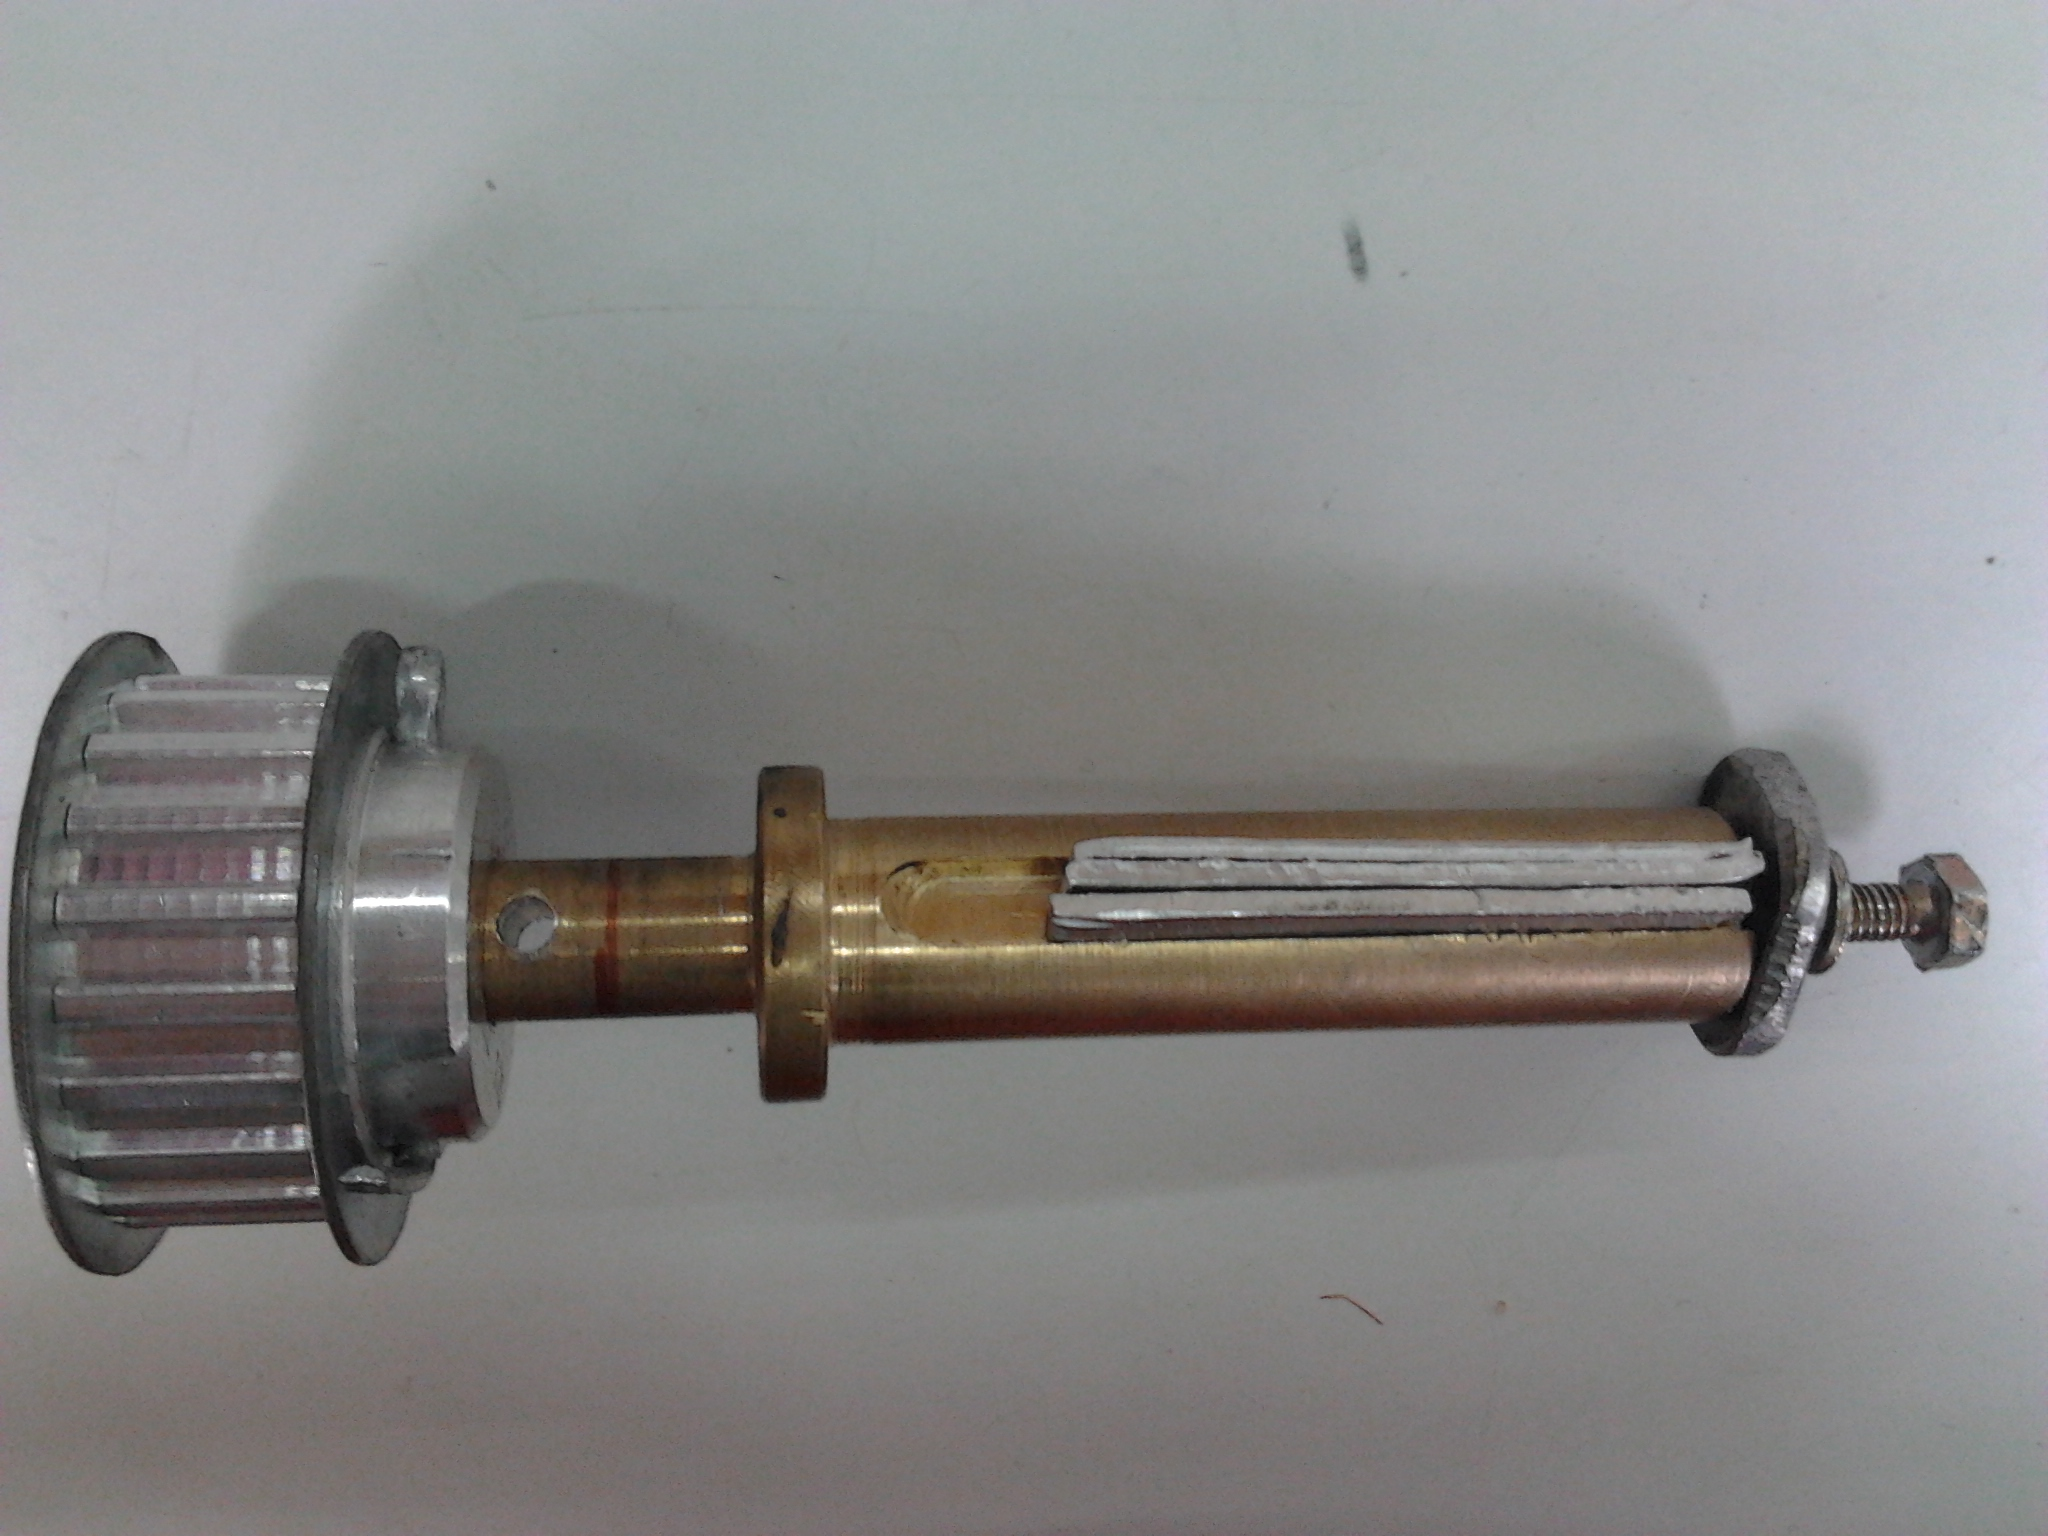
\includegraphics[width=\linewidth]{recursos/imagens/apendicef/dir_veio_redutor} }
\end{subfigure}
\qquad
\begin{subfigure}[b]{.45\linewidth}
    \subcaptionbox{Interruptor de fim de curso da dire��o com a patilha dobrada, devido � descalibra��o da roda dentada fixa na coluna da dire��o.\label{fig:dir_fc_dobrado}}{\includegraphics[width=\linewidth]{recursos/imagens/apendicef/dir_fc_dobrado} }
\end{subfigure}
\par\bigskip
\begin{subfigure}[b]{.45\linewidth}
    \subcaptionbox{Uma das duas placas acr�licas onde fixam as placas eletr�nicas presentes na caixa.\label{fig:elet_acrilico_suporte}}{\includegraphics[width=\linewidth]{recursos/imagens/apendicef/elet_acrilico_suporte} }
\end{subfigure}
\qquad
\begin{subfigure}[b]{.45\linewidth}
    \subcaptionbox{Microcontrolador instalado no ve�culo com liga��o por porta s�rie.\label{fig:elet_dalf_serie}}{\includegraphics[width=\linewidth]{recursos/imagens/apendicef/elet_dalf_serie}}
\end{subfigure}
\end{figure}
%next page
\begin{figure}[t]
\ContinuedFloat
\begin{subfigure}[b]{.45\linewidth}
    \subcaptionbox{Placa de circuito impresso do sensor de velocidade.\label{fig:encoder_pcb}}{\includegraphics[width=\linewidth]{recursos/imagens/apendicef/encoder_pcb} }
\end{subfigure}
\qquad
\begin{subfigure}[b]{.45\linewidth}
    \subcaptionbox{Redutor da tra��o, instalado.\label{fig:3_4_tras}}{\includegraphics[width=\linewidth]{recursos/imagens/apendicef/vista_3_4_tras} }
\end{subfigure}
\par\bigskip
\begin{subfigure}[b]{.45\linewidth}
    \subcaptionbox{Alinhamento da montagem dos motores da tra��o e do trav�o.\label{fig:trv_trc}}{\includegraphics[width=\linewidth]{recursos/imagens/apendicef/vista_tras_bxo} }
\end{subfigure}
\qquad
\begin{subfigure}[b]{.45\linewidth}
    \subcaptionbox{Ve�culo, visto de tr�s.\label{fig:vista_tras}}{\includegraphics[width=\linewidth]{recursos/imagens/apendicef/vista_trs} }
\end{subfigure}
\end{figure}
\cleardoublepage

		\cleardoublepage
	\end{appendix}
\end{appendices}

\todos  %list of things to do - should be the last todo item on the document
\end{document}
